\chapter{$D^0 \to \mu^+\mu^-$ Branching Fraction Measurement}
\label{ch:4}

\section{Analysis overview}

\label{sec:analysis_overview}

The goal of this analysis is to measure the branching fraction of the $D^0 \to \mu^+ \mu^-$ decay, notated as $\mathcal{B}(D^0 \to \mu^+ \mu^-)$. In performing this calculation, there are three major challenges that this analysis is faced with. 

The first, and most fundamental, of these challenges is a small signal presence compared to a large combinatorial background, due to rarity of the $D^0 \to \mu^+ \mu^-$ decay. In order to address this, we use $D^0$ mesons that originated from $D^{*\pm} \to D^0 \pi^\pm$ decays, allowing us to use the additional soft pion to better reconstruct and select for signal events. By using $D^*$ decay, we decrease the number of available $D^0 \to \mu^+ \mu^-$ signal events, but also reduce the combinatorial background by a much larger factor, improving the overall quality of the analysis. 

The second of these challenges is caused by the solution to the first. Namely, the $D^*$ cross-section is not well known at CMS, making it difficult to compute the number of $D^0$ mesons in our dataset directly. Therefore, instead we use a normalization channel approach, where we count the number of events in a normalization channel with a well known branching fraction, which we pick to be $D^0 \to \pi^+ \pi^-$ due to the kinematic similarity to the $D^0 \to \mu^+ \mu^-$ decay. Therefore, the result for this analysis is obtained by extracting out $\mathcal{B}(D^0 \to \mu^+ \mu^-)$ from the following formula.
\begin{equation}
    \frac{N_{D^0 \to \mu^+  \mu^-}}{N_{D^0 \to \pi^+ \pi^-}} = \frac{\mathcal{B}(D^0 \to \mu^+ \mu^-)}{\mathcal{B}(D^0 \to \pi^+ \pi^-)}\times \frac{\epsilon_{D^*, D^0\to\mu\mu}}{\epsilon_{D^*, D^0\to\pi\pi}} \times S_{ZB} \times \text{MVA}_D \times T_{\text{corr}} 
\label{eq:main_analysis}
\end{equation}
where $\mathcal{B}(D^0 \to \pi^+ \pi^-)$ is well known \cite{ref:pdg2024}, $N_{D^0 \to \mu^+  \mu^-}$ and $N_{D^0 \to \pi^+ \pi^-}$ are calculated using fits to data as described in section \ref{sec:UML}, $\epsilon_X$ is the efficiency of our selection calculated from Monte Carlo described in section \ref{sec:selections_and_efficency}, $S_{ZB}$ is a scale factor of the data discussed in section \ref{sec:triggers_and_datasets}, and $\text{MVA}_D,T_{\text{corr}}$ are corrections described in section \ref{sec:efficiency_corrections}. This solution also has a nice property of canceling many of the errors that exist in both channels, reducing overall systematic error and providing a simpler analysis strategy.

The third of these challenges is caused by in-flight $\pi \to \mu \nu$ decays, which cause pions to be misreconstructed or "faked" as muons. Due to the nature of this experiment in measuring pion and muon final states, the effect of the fake rate impacts elements of the entire analysis. To address the fake muon, this analysis performs an extensive analysis of the muon fake rate in section \ref{sec:muon_fake_rate}. 

Lastly, to prevent analysis design from biasing the result through effects such as overfitting to statistical fluctuations or selection bias, the entirety of the analysis is designed while being blind to the signal in data. Due to the small expected signal yield, the analysis is able to consider 1/8th of the full dataset during its design while still being considered blind. Only once the entire analysis has been laid out, is it able to consider the full dataset, which is discussed in the final section of this analysis, section \ref{subsec:final_result}. 

\section{Triggers and datasets}
\label{sec:triggers_and_datasets}

\subsection{Data samples}

\label{subsec:data_samples}

The events used for this analysis are collected from proton-proton collisions at the LHC at a center of mass of 13.6 TeV. Specifically, we use data from the CMS detector during the years 2022 and 2023. The CMS collaboration marks specific run ranges as good runs and groups them into datasets marked with letters. The data we use is denoted as 2022C, 2022D, 2022E, 2022F, 2022G, 2023C, and 2023D, with letters used to mark specific eras, or ranges of runs where the detector conditions were relatively unchanged. 

There are two triggers used for the analysis:
\begin{enumerate}
    \item The \texttt{HLT\_DoubleMu4\_3\_LowMass} trigger is used to collect $D^{*\pm} \to D^0 \pi^\pm, D^0 \to \mu^+ \mu^-$ signal events by triggering on the dimuon final product. During the collection of the data samples of the analysis, the trigger was virtually unchanged and unprescaled, making it convenient to use for signal collection.
    \item The \texttt{HLT\_ZeroBias} trigger was used to collect $D^{*\pm} \to D^0 \pi^\pm, D^0 \to \pi^+ \pi^-$ normalization events. Unlike the signal trigger, this trigger does not filter for a specific signature. However, the branching fraction of $D^{*\pm} \to D^0 \pi^\pm, D^0 \to \pi^+ \pi^-$ is large enough to generate a sufficient number of desired events. During the collection of the data samples of the analysis, the trigger was virtually unchanged.
\end{enumerate}

Due to the fact that the \texttt{HLT\_ZeroBias} trigger does not filter for a specific signature, it is exposed to much more data than any other dataset. The trigger quite literally collects data on every bunch crossing that occurs at CMS. As discussed in section \ref{sec:triggers}, this is far too much data to be processed by any modern day computer. Therefore, a \textit{prescaling} is used to keep only a select fraction of the events. This prescaling factor is incredibly important; a prescale factor of 100 means that there exists 100 times more events that satisfying the \texttt{HLT\_ZeroBias} requirements than reported in the dataset. The prescaling factor is set to be roughly $10^{6}$ and then measured experimentally by comparing the integrated lumonisty of the data. Recall that luminosity was defined earlier in equation \ref{eq:luminosity}. 

Specifically, for this experiment we calculate the ZeroBias scale factor, $S_{ZB}$ as 
\begin{equation}
    S_{ZB} = \frac{\text{total luminosity}}{\text{ZeroBias luminosity}}.
\end{equation}
Table \ref{tab:int_lumi_final} shows the measured integrated luminosity for each era. Using this, we can calculate that the total scale factor is $S_{ZB} = 1.255 \times 10^6$.

\begin{table}[htbp]
    \centering
    \begin{tabular}{|l|c|c|}
        \hline
         & \multicolumn{2}{c|}{Integrated luminosity} \\
        \cline{2-3}
         & HLT\_DoubleMu4\_3\_LowMass, fb$^{-1}$ & HLT\_ZeroBias, nb$^{-1}$ \\
        \hline
        Run2022C      & 6.155  & 6.476 \\
        Run2022D      & 3.283  & 1.395 \\
        Run2022E      & 5.939  & 4.756 \\
        Run2022F      & 18.124 & 13.482 \\
        Run2022G      & 3.084  & 2.256 \\
        \hline
        Run2022 Total & 36.585 & 28.365 \\
        \hline
        Run2023C      & 18.300 & 15.08 \\
        Run2023D      & 9.640  & 7.970 \\
        \hline
        Run2023 Total & 27.940 & 23.050 \\
        \hline
        Run2022 + Run2023 Total & 64.525 & 51.415 \\
        \hline
    \end{tabular}
    \caption{Integrated luminosity of data collected with the primary triggers.}
    \label{tab:int_lumi_final}
\end{table}

The events collected by these two triggers and grouped into two datasets, ZeroBias and Parking DoubleMuonLowMass, respectively. We use the NanoAOD file format, designed by CMS to contain ntuples of per-event information and used for most analysis at CMS. Specifically, we use the NanoAODv12 recipe which is processed from MiniAOD. In this processing, we apply the muon data certification to ensure high quality muon objects. 

\subsection{Backgrounds}
\label{subsec:backgrounds}

A key component of the analysis is the accurate modeling of background, specifically because of how small the anticipated limit of the signal strength is. There are two main types of backgrounds to consider: 
\begin{enumerate}
    \item Combinatorial backgrounds: backgrounds which are characterized by noise from random combinations of particles produced in secondary particle collisions. 
    \item Peaking backgrounds: backgrounds which are characterized by random combinations of particles produced in the same event.
\end{enumerate}

\subsubsection{Combinatorial Backgrounds}

Combinatorial backgrounds are signals that originate from random combinations of particles that do not come from a common physical process. The existence of combinatorial backgrounds is present in virtually every experiment performed at the LHC due to the large amounts of events generated in each proton-proton bunch collision. Combinatorial backgrounds are often characterized by smooth, non-peaking shapes due to the lack of a unifying physical process to generate a peak. There are many shapes that are used to fit to combinatorial backgrounds, with the most common being exponential functions or polynomial functions. The functions allow for the needed degrees of freedom and overall shape to converge on the smooth combinatorial shape. In other applications, more specific combinatorial functions are derived to properly model the background. 

\subsubsection{Peaking Backgrounds}

Unlike combinatorial backgrounds, peaking backgrounds must be carefully studied to ensure that the background peak in the signal region is not modeled as signal. These peaking backgrounds occur most commonly from detector misreconstruction. For example, pions can be misreconstructed as muons, resulting in some $D^0 \to \pi^+ \pi^-$ events being reconstructed as $D^0 \to \mu^+ \mu^-$ events, causing a peaking background near the signal peak. Specifically, we know that pions and kaons are the only 2 particles which are (1) common decay products of the $D^0$ and (2) are relatively frequently misreconstructed as muons\footnote{See section \ref{sec:muon_fake_rate}}. Therefore, the candidates for peaking background are two body hadronic decays of the $D^0$ meson and non-$D^{*\pm} \to D^0 \pi^\pm$ decays. 

For each of the peaking backgrounds, we check their $\Delta m$ and dimuon mass against the $\Delta m$ and dimuon mass of the signal. While the non-$D^{*\pm} \to D^0 \pi^\pm$ decays exhibit a dimuon mass distribution which is virtually identical to the signal, their $\Delta m$ contribution is expected to be combinatorial so they do not overlap with the signal's signature. The dominate two body hadronic decays of the $D^0$ meson therefore are the only contributions to peaking background and are listed below.
\begin{enumerate}
    \item $D^0 \to \pi^+ \pi^-$
    \item $D^0 \to K^\pm \pi^\mp$
    \item $D^0 \to K^+ K^-$
    \item $D^0 \to \pi^- \mu^+ \nu_\mu$\footnote{Due to the semileptonic nature of this decay, it only have a peaking structure in $m(D^0)$, only in $\Delta m$}
\end{enumerate}
For each of these, we use \texttt{TGenPhaseSpace} to simulate the effects of the misreconstructed on the peaking background distributions in both $\Delta m$ and the invariant dimuon mass and compare them to the signal distribution. As can be seen in figure \ref{fig:reconstructed_D0_comparison}, every decay except $D^0 \to \pi^+ \pi^-$ gives a distribution which is distinct from the signal distribution in either $\Delta m$ or the dimuon invariant mass. Therefore, the only peaking distribution which we must model and account for is $D^0 \to \pi^+ \pi^-$. 

\begin{figure}[htp]
    \begin{center}
      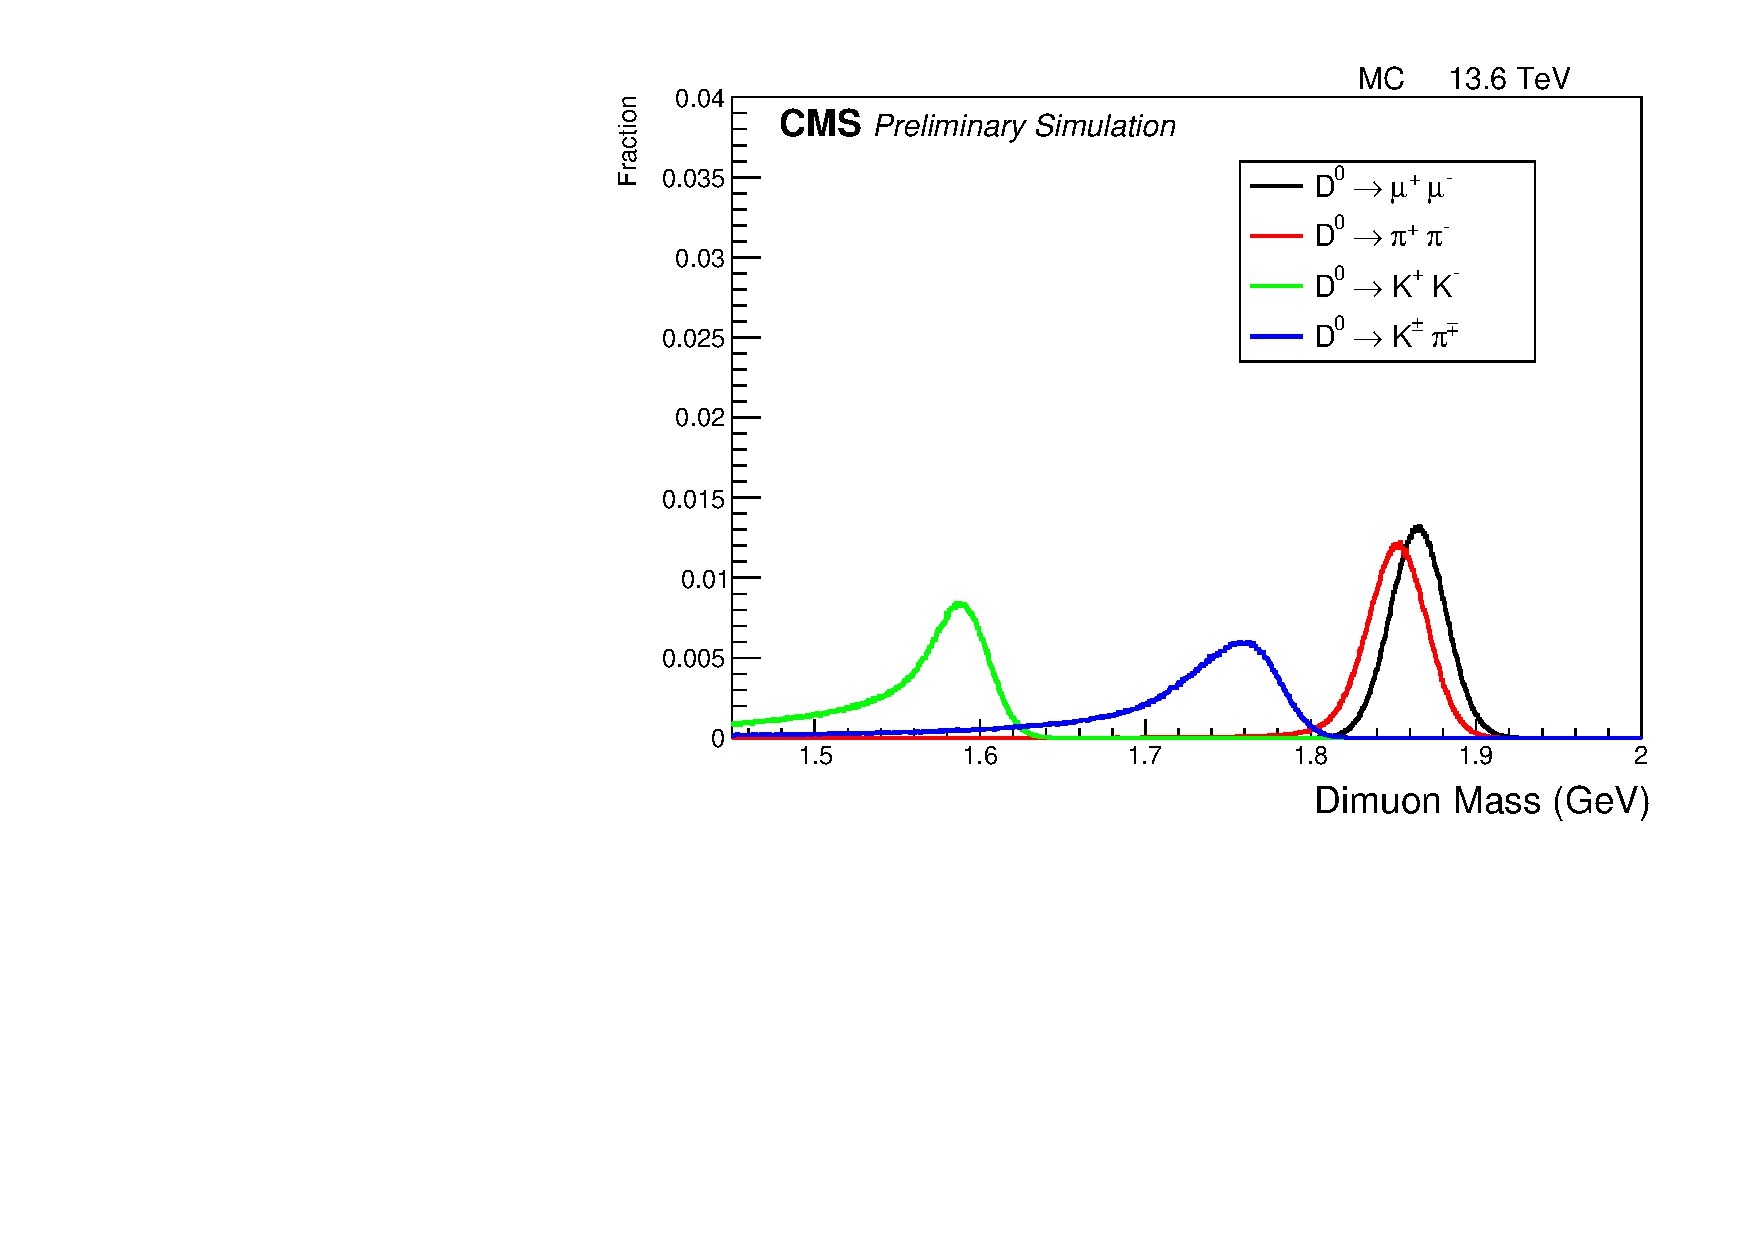
\includegraphics[width=0.45\textwidth]{figures/chapter4/reconstructed_D0_mass.pdf}
      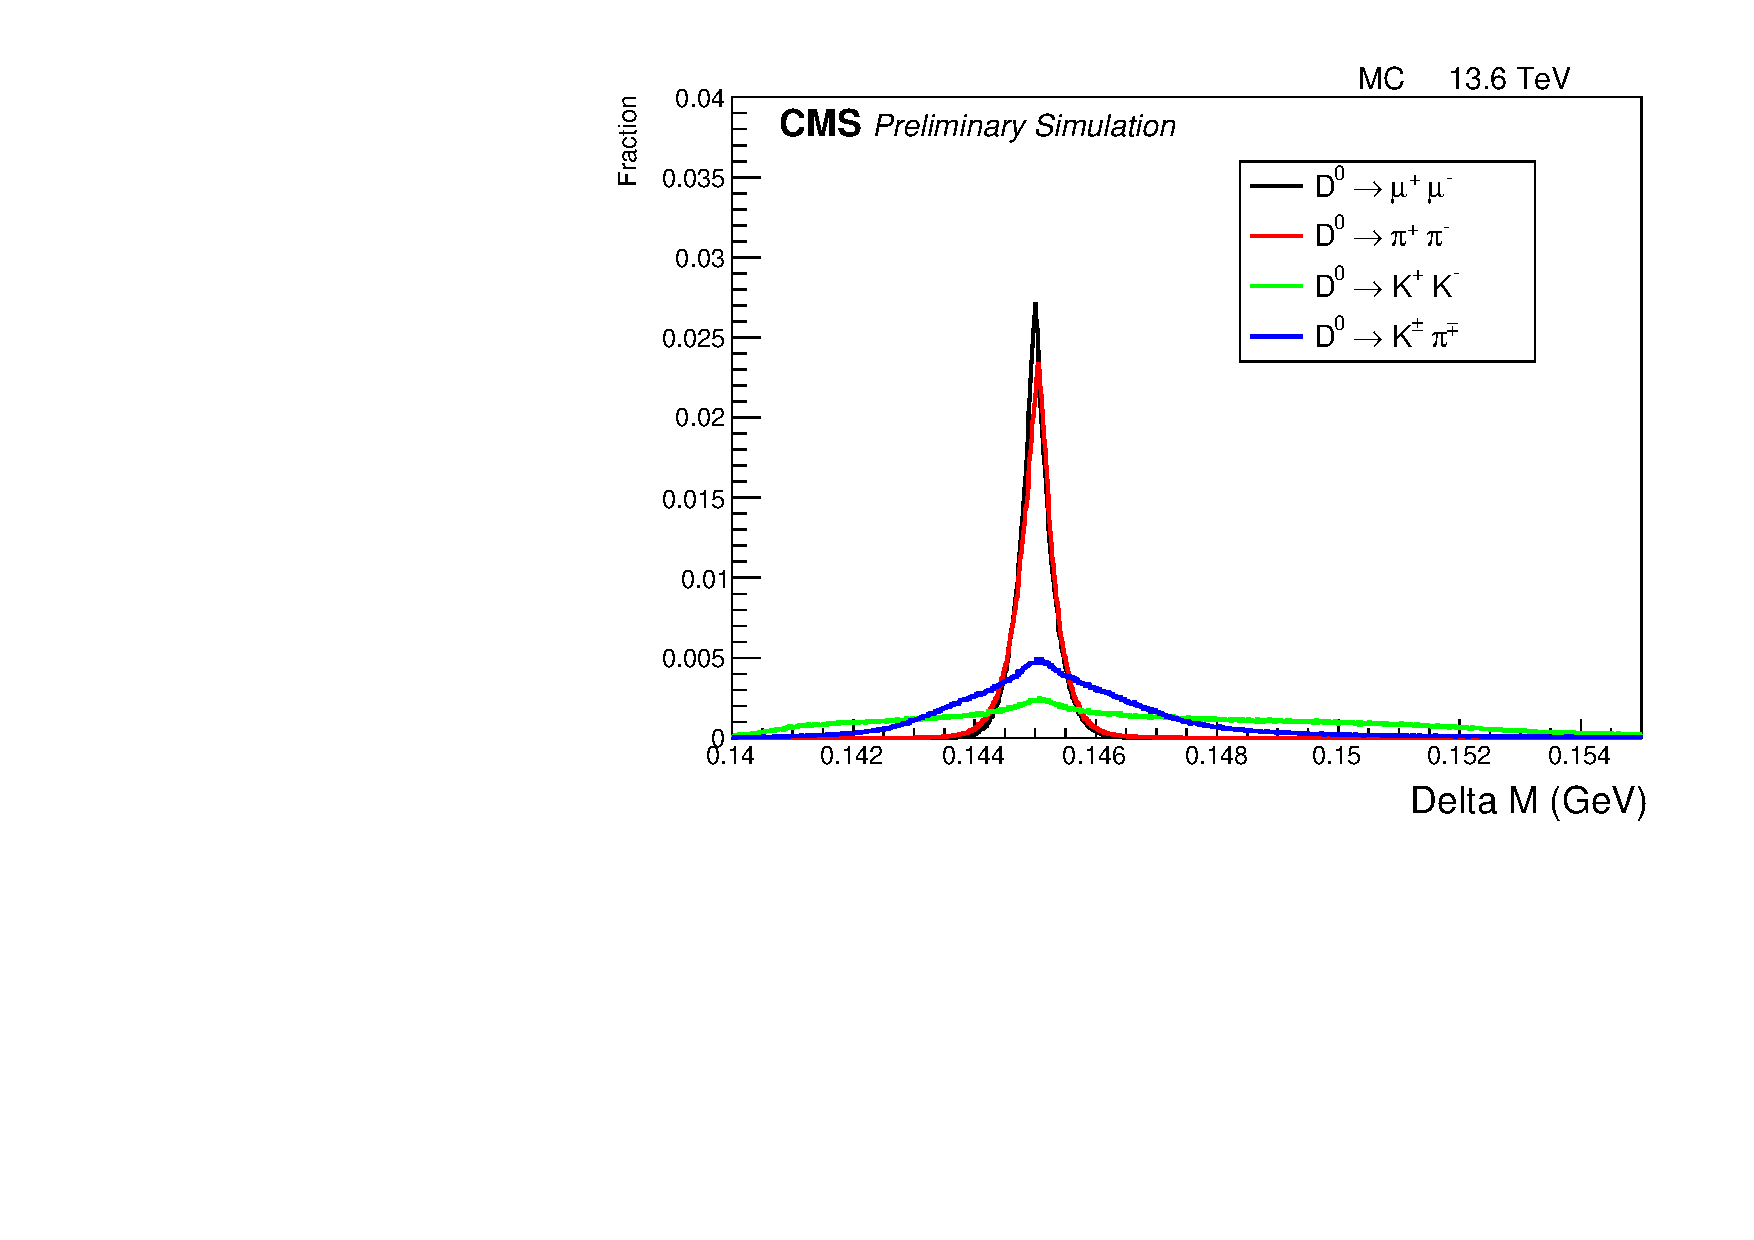
\includegraphics[width=0.45\textwidth]{figures/chapter4/reconstructed_delta_m.pdf}\\
    \end{center}
    \caption{
      Comparison of normalized frequencies for various peaking background $D^0 \to \mu^+ \mu^-$ decays against the signal decay.
      Right: Reconstructed $\Delta m$ distribution.
      Left: Reconstructed dimuon mass distribution, where decay products are forced to take the muon mass using \texttt{TGenPhaseSpace}, even for non-dimuon final states.
    }
    \label{fig:reconstructed_D0_comparison}
  \end{figure}
  
  


\subsection{Monte Carlo samples}

The main component of constructing the Monte Carlo (MC) simulation samples is properly modeling the $D^*$ meson by replicating their production in the CMS detector. The $D^*$ has two primary production mechanisms at the LHC
\begin{enumerate}
    \item Production through hadronization of charm quark directly from the proton-proton collision, creating prompt $D^*$ mesons close to the primary vertex. 
    \item Production through decay of other $B$ hadrons, creating displaced $D^*$ mesons from a secondary vertex
\end{enumerate}

It is important to model both of these production mechanisms of the $D^*$ decay to generate a reliable MC simulation sample, therefore both are included in the MC sample. Specifically, the first method produces a prompt soft pion in the $D^*\pm \to D^0 \pi^\pm$ process while the second method produces a displaced soft pion, resulting in significant differences in vertex parameters used in reconstruction and classification. The full complexity of the MC samples extends beyond the scope of this thesis, but table \ref{tab:mc-samples} displays some of the most used samples.

\begin{table}
\centering
\begin{tabular}{|p{3.2cm}|p{12cm}|}
    \hline
    \textbf{Sample Name} & \textbf{Attributes} \\
    \hline
    DstarToD0Pi\_ & -- SoftQCD:nonDiffractive (MinBias) \\
    D0To2Mu\_ & -- force $D^* \to D^0\pi$, $D^0 \to \mu^+\mu^-$ decay \\
    MuFilter & -- $|\eta(D^*)| < 3.0$ \\
    & -- $|\eta(D^0)| < 3.0$ for $D^0$ from $D^*$ \\
    & -- $|\eta| < 2.6$, $p_T > 3.0$ for muons from $D^0$ \\
    \hline
    DstarToD0Pi\_ & -- SoftQCD:nonDiffractive (MinBias) \\
    D0To2Pi\_ & -- force $D^* \to D^0\pi$, $D^0 \to \pi^+\pi^-$ decay \\
    PiFilter & -- $|\eta(D^*)| < 3.0$ \\
    & -- $|\eta(D^0)| < 3.0$ for $D^0$ from $D^*$ \\
    & -- $|\eta| < 2.6$, $p_T > 3.0$ for pions from $D^0$ \\
    \hline
    DstarToD0Pi\_ & -- SoftQCD:nonDiffractive (MinBias) \\
    D0ToKPi\_ & -- force $D^* \to D^0\pi$, $D^0 \to K^-\pi^+$ decay \\
    KPiFilter & -- $|\eta(D^*)| < 3.0$ \\
    & -- $|\eta(D^0)| < 3.0$ for $D^0$ from $D^*$ \\
    & -- $|\eta| < 2.6$, $p_T > 3.0$ for pions from $D^0$ \\
    \hline
    DstarToD0Pi\_ & -- SoftQCD:nonDiffractive (MinBias) \\
    D0To2Pi\_ & -- force $D^* \to D^0\pi$, $D^0 \to \pi^+\pi^- \to \mu^+\nu_\mu\mu^-\nu_\mu$ \\
    PiToMuPiFilter\_ & -- reduce pion $c\tau$ from 7.8\,m to 15.6\,cm \\
    PiLifetime0p02 & -- pion decay limits: $R < 2$\,m, $|z| < 4$\,m \\
    & -- $|\eta(D^*)| < 3.0$ \\
    & -- $|\eta(D^0)| < 3.0$ for $D^0$ from $D^*$ \\
    & -- $|\eta| < 2.6$, $p_T > 3.0$ for pions from $D^0$ \\
    & -- $|\eta| < 2.6$, $p_T(\mu) > 3.0$ for muons from pions \\
    \hline
\end{tabular}
\caption{The 4 most relevant MC simulation samples and their defining attributes.}
\label{tab:mc-samples}
\end{table}

\section{Selections and efficiency}
\label{sec:selections_and_efficency}

Once we've attained the data and MC samples needed for this analysis, we filter through them using event selections, carefully tracking the \textit{acceptance} and \textit{efficiency} for each selection\footnote{We define \textit{acceptance} as the purely kinematic fraction of signal events that fall inside the geometric phase space of the analysis and \textit{efficiency} as the analysis' performance in identifying signal events that are inside the geometric region}. The selection process can be broken down into three main stages:
\begin{enumerate}
    \item The \textit{preselection} stage provides the selections which are tied to trigger requirements, reconstruction requirements, and dataset size limitations.
    \item The \textit{baseline selection} stage primarily is used to reject background samples while keeping the efficiency high, the sidebands of the signal region large, and the signal shape unperturbed. 
    \item The \textit{multivariate analysis (MVA) selection} stage uses ML-methods to optimize the background rejection.
\end{enumerate}

\subsection{Preselection}
\label{subsec:preselection}

The preselection is used to create reconstructed event candidates which pass the triggers discussed in section \ref{subsec:data_samples}. To stay consistent between signal and normalization events, we keep a similar preselection process for both $D^{*\pm} \to D^0 \pi^\pm, D^0 \to \mu^+ \mu^-$ and $D^{*\pm} \to D^0 \pi^\pm, D^0 \to \pi^+ \pi^-$ events.

In order to properly reconstruct the $D^{*\pm} \to D^0 \pi^\pm, D^0 \to \mu^+ \mu^-$ and $D^{*\pm} \to D^0 \pi^\pm, D^0 \to \pi^+ \pi^-$ events, we first must reconstruct their decay products: the muons and pion. Pions are reconstructed from charged tracks found in the tracker. These tracks are reconstructed using particle flow (PF) algorithms\footnote{The primary goal of these algorithms is to reconstruct individual particles using the data read out from the detector itself. This is made especially difficult because of the high luminosities of run3 resulting in a large amount of \textit{pileup}, a phenomenon that occurs due to multiple proton-proton collisions happening within a very short time frame resulting in multiple collisions per event. }, meaning the pions used in the analysis are labeled as PF candidates. Muons are reconstructed primarily using detector read out from the muon chambers. We use the well established CMS reconstruction algorithms \texttt{TrackerMuon} and \texttt{GlobalMuon} as well as use the collaboration's \texttt{LooseMuonID} for muon identification. To reduce background noise and increase detector resolution, we also cut at $p_T>4$ GeV and require a \texttt{highPurity} inner track in the tracker for both pions and muons.

Once we have the muon and/or pion candidates for the $D^0$ decay, we use vertex reconstruction to reconstruct the full decay candidate. A \textit{vertex} is the location in 3D space where a process occurred and the \textit{primary vertex} is the location of the interaction of the quarks of the two colliding protons, which in our case produce the $D^{*\pm}$. Due to the short mean lifetime of the $D^{*\pm}$ ($ 6.9 \pm 1.9 \times 10^{-21} \; s$) \cite{ref:pdg2024}, we can label the $D^{*\pm} \to D^0 \pi^\pm$ vertex using the primary vertex. The kinematic vertex reconstruction begins by identifying the dimuon or dipion decay candidates fit to a common vertex (i.e two pions or two muons which came from the same decay). The two 4-momentum vectors of these two candidates is added together to get a dimuon or dipion 4-momentum vector. We call this dimuon/dipion system a $D^0$ candidate. Using the $D^0$ candidate 4-momentum vector, we calculate the transverse momentum of $D^0$ candidate and extrapolate it to its intersection with the beamline. Then, in order to determine which primary vertex\footnote{There are often many primary vertices in one event due to pileup} the $D^{*\pm} \to D^0 \pi^\pm$ decay came from, we calculate the 3D distance between each primary vertex candidate and the extrapolated intersection point, known as the \textit{3D-impact parameter}, and find the primary vertex which minimizes this parameter. Lastly, since the decay at the primary vertex is $D^{*\pm} \to D^0 \pi^\pm$, we check if there exists a soft pion which came from the selected primary vertex \cite{ref:Prokofiev_Speer_2005}. This kinematic vertex reconstruction is then used to gather reconstructed signal and normalization events as well as refit the $D^0$ candidates to a common vertex using a kinematic vertex fitting tool, generating \textit{refitted} candidates. The events which pass this reconstruction are thus the events that pass the preselection. 

\begin{figure}[htbp]
    \centering
    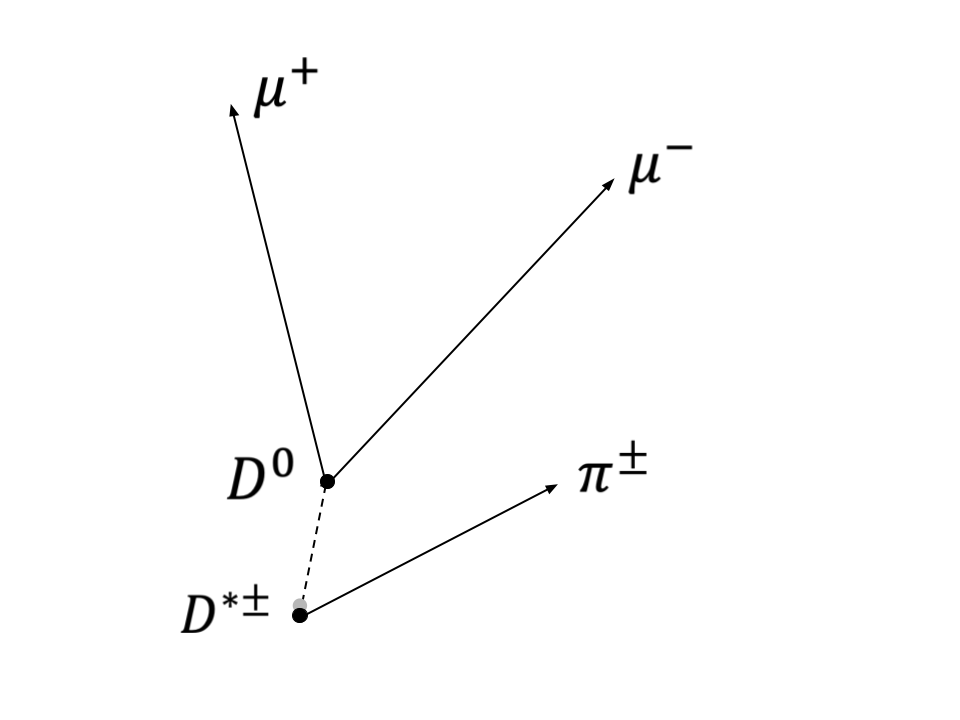
\includegraphics[width=0.8\textwidth]{figures/chapter4/vertex_reconstruction.png}
    \caption{An example of the $D^{*\pm} \to D^0 \pi^\pm, D^0 \to \mu^+ \mu^-$ vertex}
    \label{fig:vertex_reconstruction}
\end{figure}

\subsection{Baseline selection}
\label{subsec:baseline_selection}

Using the reconstruction described in section \ref{subsec:preselection}, we are able to extract several kinematic variables from $D^{*\pm} \to D^0 \pi^\pm$ candidates outputted by the preselection. These variables are used in the baseline selection as well as in other parts of the analysis. They are defined here as follows:
\begin{enumerate}
    \item Reconstructed $D^0$ mass: the mass calculated from the addition of the two 4-momentum vectors of the $D^0$'s product candidates (either dimuon or dipion). 
    \item Refitted $D^0$ mass: the mass calculated from the addition of the two 4-momentum vectors of the $D^0$'s product candidates (either dimuon or dipion) once they have been refitted using the kinematic vertex fitting. 
    \item Reconstructed $\Delta m$: the mass difference between the reconstructed $D^{*\pm}$ candidates and the reconstructed $D^0$ candidates. 
    \item Refitted $\Delta m$: the mass difference between the $D^{*\pm}$ and the $D^0$ candidates once they have been refitted using the kinematic vertex fitting.
    \item $\delta_{3D}$: the 3D impact parameter as defined in section \ref{subsec:preselection})
    \item $\delta_{3D}/\sigma\left(\delta_{3D}\right)$: the significance of the 3D impact parameter. This is calculated by taking the value of the 3D impact parameter and dividing it by the square root of the expected variance of the parameter. 
    \item $l_{3D}$: the 3D distance between the vertex of the $D^{*\pm} \to D^0 \pi^\pm$ decay (primary vertex) and the vertex of the $D^0 \to l l$ decay. This can also be called the $\textit{flight length}$ of the $D^0$ meson. 
    \item $l_{3D}/\sigma\left(l_{3D}\right)$: the significance of the 3D distance between the vertex of the $D^{*\pm} \to D^0 \pi^\pm$ decay (primary vertex) and the vertex of the $D^0 \to l l$ decay. Calculated by taking the value of the distance and dividing it by the square root of the expected variance of the distance. 
    \item $l_{xy}$: the distance in the $xy$ plane (perpendicular to the beam line) between the vertex of the $D^{*\pm} \to D^0 \pi^\pm$ decay (primary vertex) and the vertex of the $D^0 \to l l$ decay.  This can also be called the $\textit{transverse flight length}$ of the $D^0$ meson. 
    \item $l_{xy}/\sigma\left(l_{xy}\right)$: the significance of the distance in the $xy$ plane between the vertex of the $D^{*\pm} \to D^0 \pi^\pm$ decay (primary vertex) and the vertex of the $D^0 \to l l$ decay. Calculated by taking the value of the distance and dividing it by the square root of the expected variance of the distance. 
    \item $\alpha_{3D}$ : the angle between the $D^0$ momentum and flight direction. 
    \item $D^0$ vertex probability: the probability given by the $\chi^2$ fit which reconstructs the $D^0$ vertex 
    \item $D^*$ vertex probability: the probability given by the $\chi^2$ fit which reconstructs the $D^*$ vertex
\end{enumerate}
Note that, unless otherwise stated, the refitted variables are used over the reconstructed ones. 

Using these variables, we impart a baseline selection on the preselected events. The goal of the baseline selection is to reject much of the background while keeping the signal efficiency high and not perturbing the signal shape. To achieve this, we select a $D^0$ reconstructed mass in the range of [1.75, 1.95], $D^0$ refitted mass in the range of [1.81, 1.94], reconstructed $\Delta m$ in the range of [0.135, 0.160], and refitted $\Delta m$ in the range [0.140, 0.150]. These ranges are picked such that there are large sidebands on the signal, keeping signal efficiency high.

The other set of baseline selections are on the vertices themselves. We require the $D^*$ vertex probability to be greater that $0.1$ and the $D^0$ vertex probability to be greater than $0.01$. This is done such that there is some confidence in the vertex reconstruction and such that we can match the double muon trigger requirement of $0.005$. To gain further confidence in the vertex reconstruction, we limit $\alpha_{3D} < 0.1$ radians and the flight length significance to be greater than 3. Lastly, to keep the normalization channel (which is gathered from a ZeroBias trigger) under the same selection as the signal channel (which is gathered from a HLT\_DoubleMuon trigger), we require the event in the normalization channel to have fired the \texttt{HLT\_DoubleMu4\_3\_LowMass} trigger. Note, this does not mean than the specific decay we reconstruct fired the trigger, in fact usually some other event has fired the trigger. 

%TODO: insert table of efficiencies


\subsection{Multivariate Analysis}
\label{subsec:mva}

The preselection and baseline selections optimize signal efficiency, but not overall analysis sensitivity. In order to optimize the analysis sensitivity, we train a classifier using a decision tree model driven multivariate analysis (MVA). This single classifying parameter can then be used as a selection parameter named $\text{MVA}_D$ and the cut can be tuned to optimize analysis sensitivity.

The decision tree model used is based on the XGBoost (Extreme Gradient Boosting) library \cite{ref:chen_Guestrin_2016}, which builds a forest of regression trees trained sequentially to minimize a regularized objective function. Each tree in the sequence focuses on correcting the errors of the previous tree and the scores from the trees are combined to get a final prediction on the classification of the event from the forest. Each tree is constructed using a greedy algorithm that selects splits based on gain, with regularization terms penalizing model complexity to prevent overfitting. The loss function is binary logistic loss, which is optimized using boosting under second-order gradient information with an evaluation metric based on the area under the receiver-operating characteristic (ROC) curve, known as AUC in the literature. Each tree has a maximum depth of 3 and is trained using a learning rate of $\eta = 0.1$. An additional regularization is applied with an L1 penalty. A minimum loss reduction threshold for tree splits\footnote{This requirement only allows additional trees to form if their contribution causes the loss to decrease by some number, set in this analysis to be $2.0$} and a sub-sample ratio\footnote{This is the fraction of training data that each tree sees, which for this analysis is kept (as is standard) at $60\%$} are employed to additionally prevent overfitting. The model is trained for over 4000 epochs in each training round.

The signal events used for training are taken from simulated $D^0 \to \mu^+ \mu^-$ MC samples. The background events are taken from the data sidebands using the $\Delta m$ parameter with a distance of over $5\sigma$ right of the expected value ($\Delta m \in [0.150, 0.155]$ GeV) and dimuon mass in the signal range of $[1.81, 2.45]$ GeV. The dimuon mass is kept in the signal range to align the training data with not obviously rejected events. Should the background training data be selected outside the signal dimuon mass window, the classification of signal and background events would become trivial, leading to a less effective model.

The variables used in the training are
\begin{enumerate}
    \item The $p_T$ of both muons and the soft pion
    \item The $D^0$ vertex parameters, including point angle, flight length significance, vertex probability, 3D impact parameter, and significance of the 3D impact parameter.
    \item The $D^*$ vertex probability.
    \item The $D^0$ mass resolution over the $D^0$ mass.
\end{enumerate}

\begin{figure}[htp]
    \begin{center}
      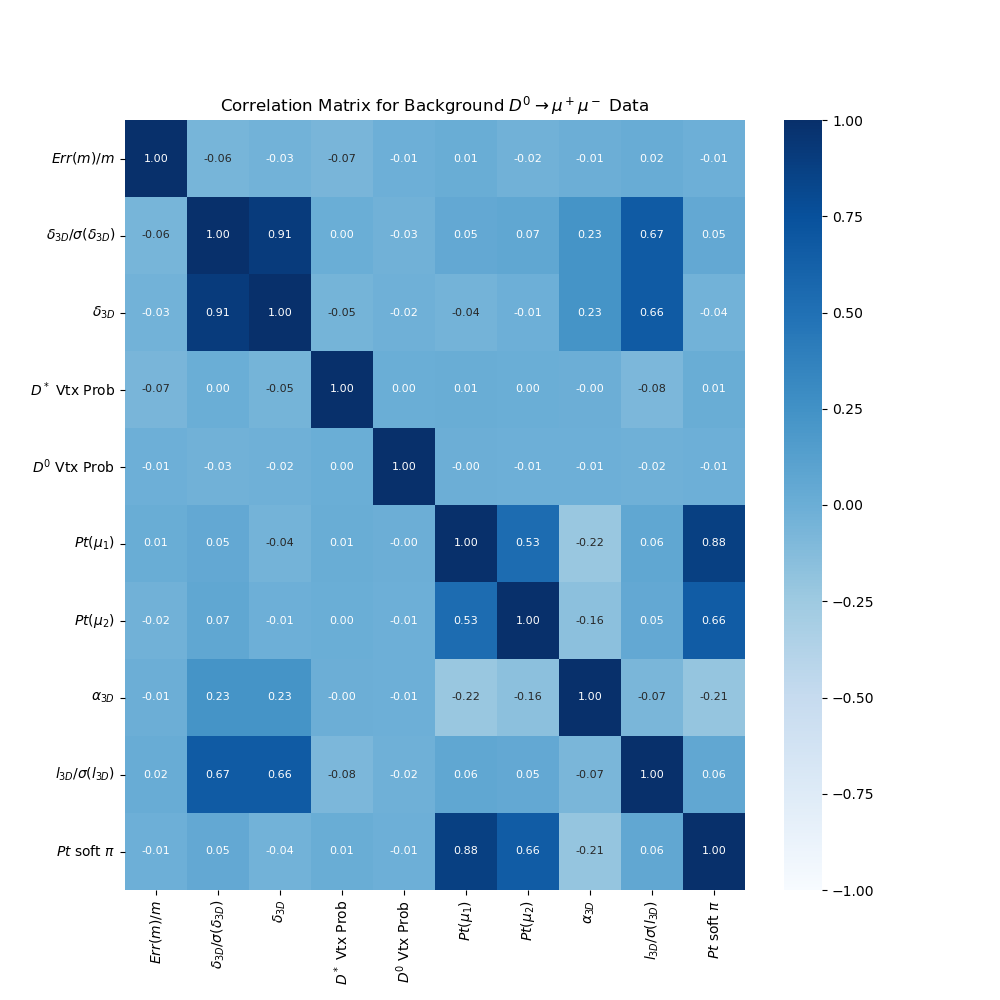
\includegraphics[width=0.45\textwidth]{figures/chapter4/mva/Correlation_data.png}
      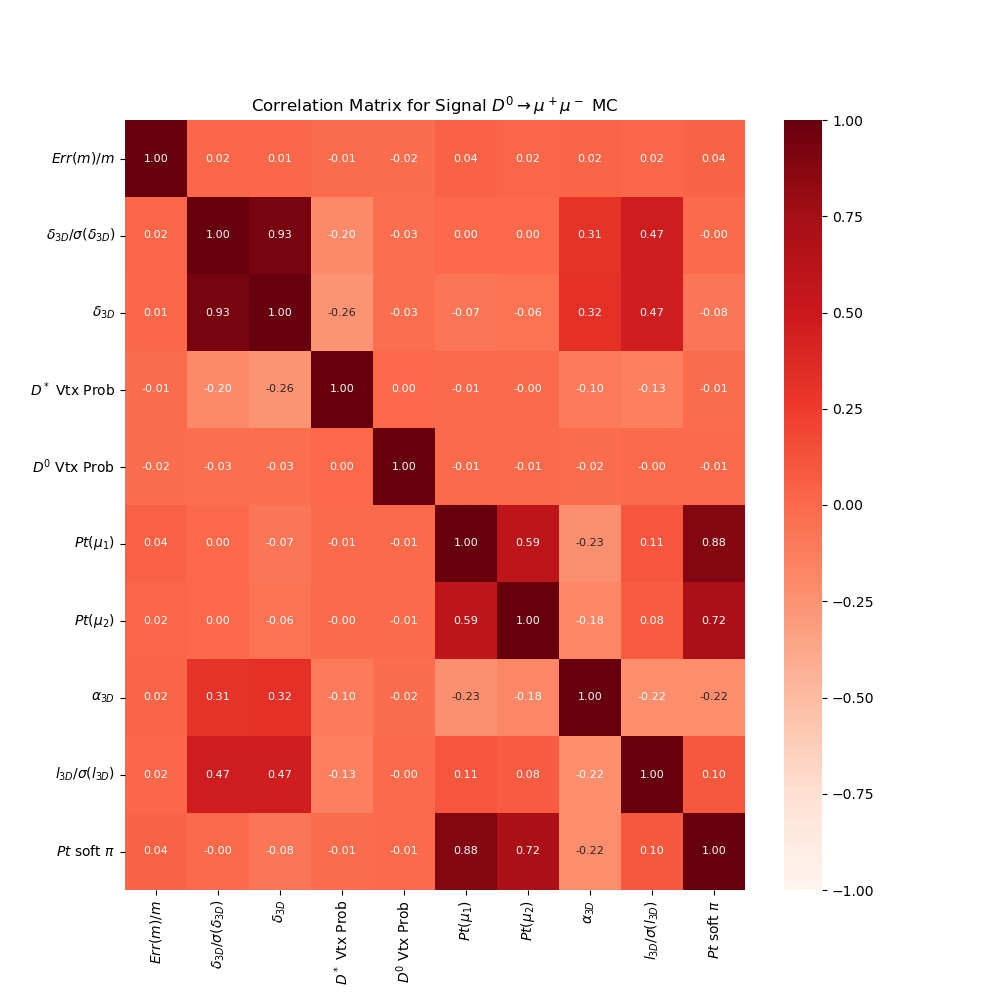
\includegraphics[width=0.45\textwidth]{figures/chapter4/mva/Correlation_dmm.png}\\
    \end{center}
    \caption{
      Correlation matrix over the MVA training variables for training background events generated from data (left) and training signal events generated from MC (right)
    }
    \label{fig:mva_correlation_matrix_for_training_variables}
\end{figure}

The correlation matrix for both the signal and background can be seen in figure \ref{fig:mva_correlation_matrix_for_training_variables}. Importantly, there are some positive correlation between features and there are no two strong anti-correlated features, meaning we expect stability in learning due to feature redundancy and simpler interactions, yet expect good model generalization. 

Due to the relatively small amount of data available, the data is split into 5 groups and 5 separate models are training, each using a different data group as testing data sets and the remaining 4 as training datasets. This ensures the models have been exposed on the entire dataset while not overfitting on any particular events. Once the models have been trained, the event number (which is independent of the contents of the event), is used to decide which model to use for classification of that event. 

It is important that the classification parameter is not correlated with any variables used later in the analysis for fitting (namely $\Delta m$ and the dimuon mass) so as to not skew the fit. Due to this, the kinematic variable given to the model are restricted to $p_T$ and vertex parameters, so that it is not possible to reconstruct masses. To check that the correlations don't exist, a correlation matrix between the classification parameter, $\Delta m$, and the dimuon mass is created and shown in figure \ref{fig:mva_correlation_matrix_for_fit_variables}. As expected, there is no correlation.


\begin{figure}[htp]
    \begin{center}
      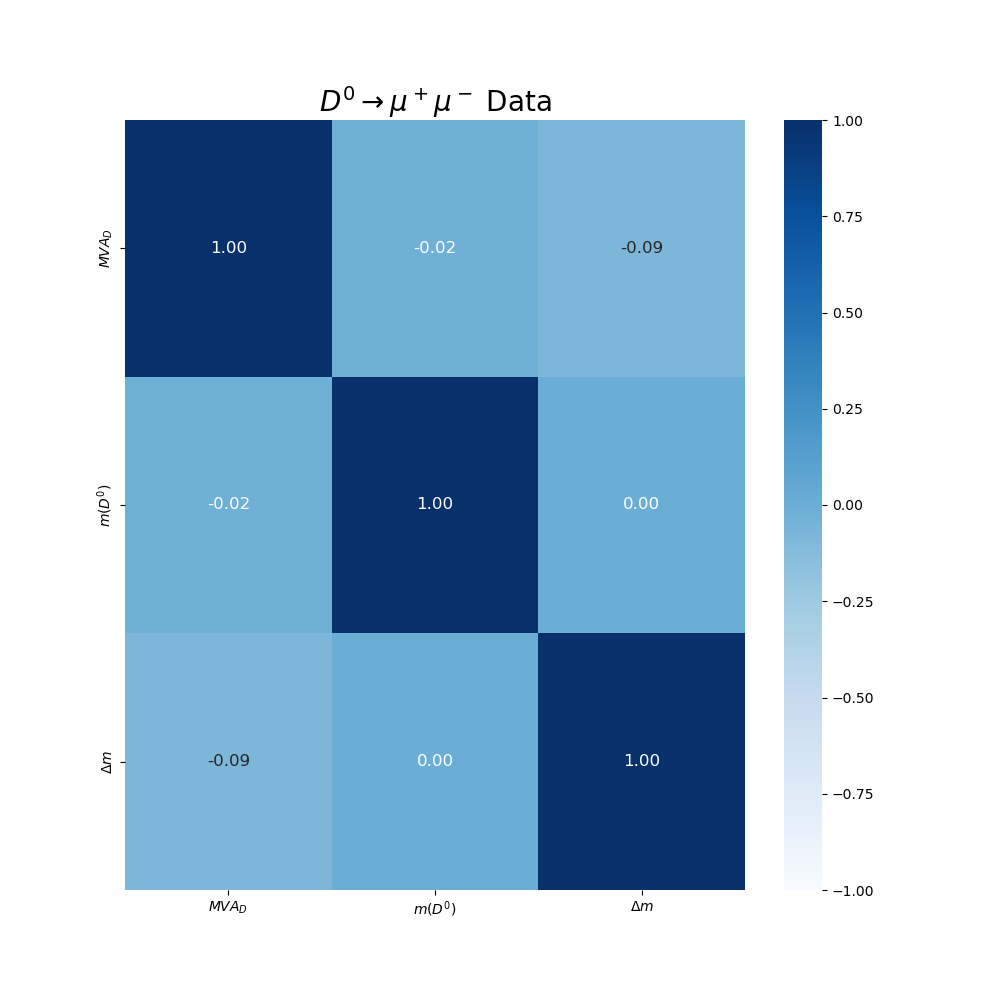
\includegraphics[width=0.45\textwidth]{figures/chapter4/mva/Correlation_data_obs.png}
      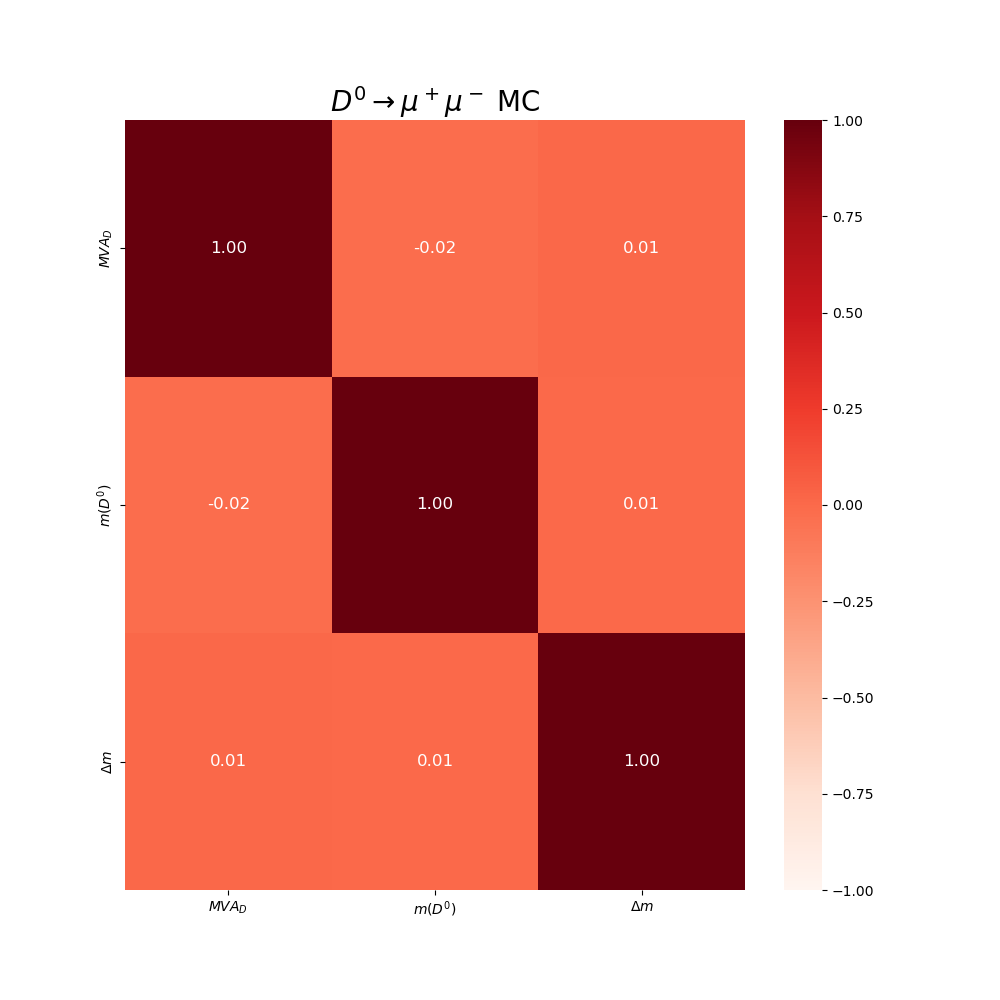
\includegraphics[width=0.45\textwidth]{figures/chapter4/mva/Correlation_dmm_obs.png}\\
    \end{center}
    \caption{
      Correlation matrix comparing the MVA classification parameter to $\Delta m$ and the dimuon mass. Shown left is the training background events generated from data and shown right is the training signal events generated from MC.
    }
    \label{fig:mva_correlation_matrix_for_fit_variables}
\end{figure}



% TODO: add statement about how efficiency is calculated in this analysis using simulated data
It is also important to note that the classifier is being trained and tested on simulated signal samples, yet for the analysis the efficiency of the classifier on real data is needed. Due to mismodeling effect in the simulation, the simulation efficiency is not necessarily the same as the data efficiency. Getting the efficiency is difficult to measure directly since the expected branching fraction of $D^0 \to \mu^+ \mu^-$ is so low that we do not have a reliable data sample for the signal. Instead, the efficiency is derived from the $D^0 \to \pi^+ \pi^-$ decay using the zero bias dataset and the $D^0 \to \pi^+ \pi^-$ monte-carlo simulation samples. Since the $D^0 \to \pi^+ \pi^-$ decay behaves similarly to the $D^0 \to \mu^+ \mu^-$ decay in terms of reconstruction/vertex parameters and the MVA classifier is independent of $\Delta m$ and dimuon mass in both cases, the efficiency derived from $D^0 \to \pi^+ \pi^-$ is similar to the efficiency of $D^0 \to \mu^+ \mu^-$. Therefore, the same classifier with the same cut is used on both the normalization channel and the signal channel, causing the $\text{MVA}_D$ efficiencies to cancel in the branching fraction equation (equation \ref{eq:main_analysis}). We calculate the efficiency in data on the $D^0 \to \pi^+ \pi^-$ decay by performing the UML fit outlined in section \ref{subsec:normalization_channel_fit} on different $\text{MVA}_D$ cut values and comparing to the \texttt{ZeroBias} dataset. In simulated data, we are able to directly tag the signal events that were created from the simulation, so calculating the efficiency is trivial. A list of efficiency values at specific $\text{MVA}_D$ cuts can be found in table \ref{tab:mva_cut_efficiencies} and a graphical representation over a more diverse $\text{MVA}_D$ cut range can be found in \ref{fig:mva_cut_efficiencies}.

\begin{table}[htbp]
    \centering
    \begin{tabular}{|l|c|c|c|}
    \hline
    $\text{MVA}_D$ cut value & \textbf{0.74} & \textbf{0.76} & \textbf{0.78} \\
    \hline
    $D^0 \to \pi^+ \pi^-$ Data Efficiency (from Zero Bias) & $0.722 \pm 0.088$ & $0.707 \pm 0.087$ & $0.681 \pm 0.086$ \\
    $D^0 \to \pi^+ \pi^-$ MC Efficiency & 0.817 & 0.801 & 0.783 \\
    $D^0 \to \mu^+ \mu^-$ MC Efficiency & 0.824 & 0.809 & 0.792 \\
    $D^0 \to \pi^+ \pi^- \to \mu^+\nu_\mu\mu^-\bar{\nu}_\mu$ MC Efficiency & 0.806 & - & - \\
    \hline
    \end{tabular}
    \caption{Summary of $\text{MVA}_D$ cut efficiency at various cut values on various samples used throughout the analysis.}
    \label{tab:mva_cut_efficiencies}
\end{table}

\begin{figure}[htp]
    \begin{center}
      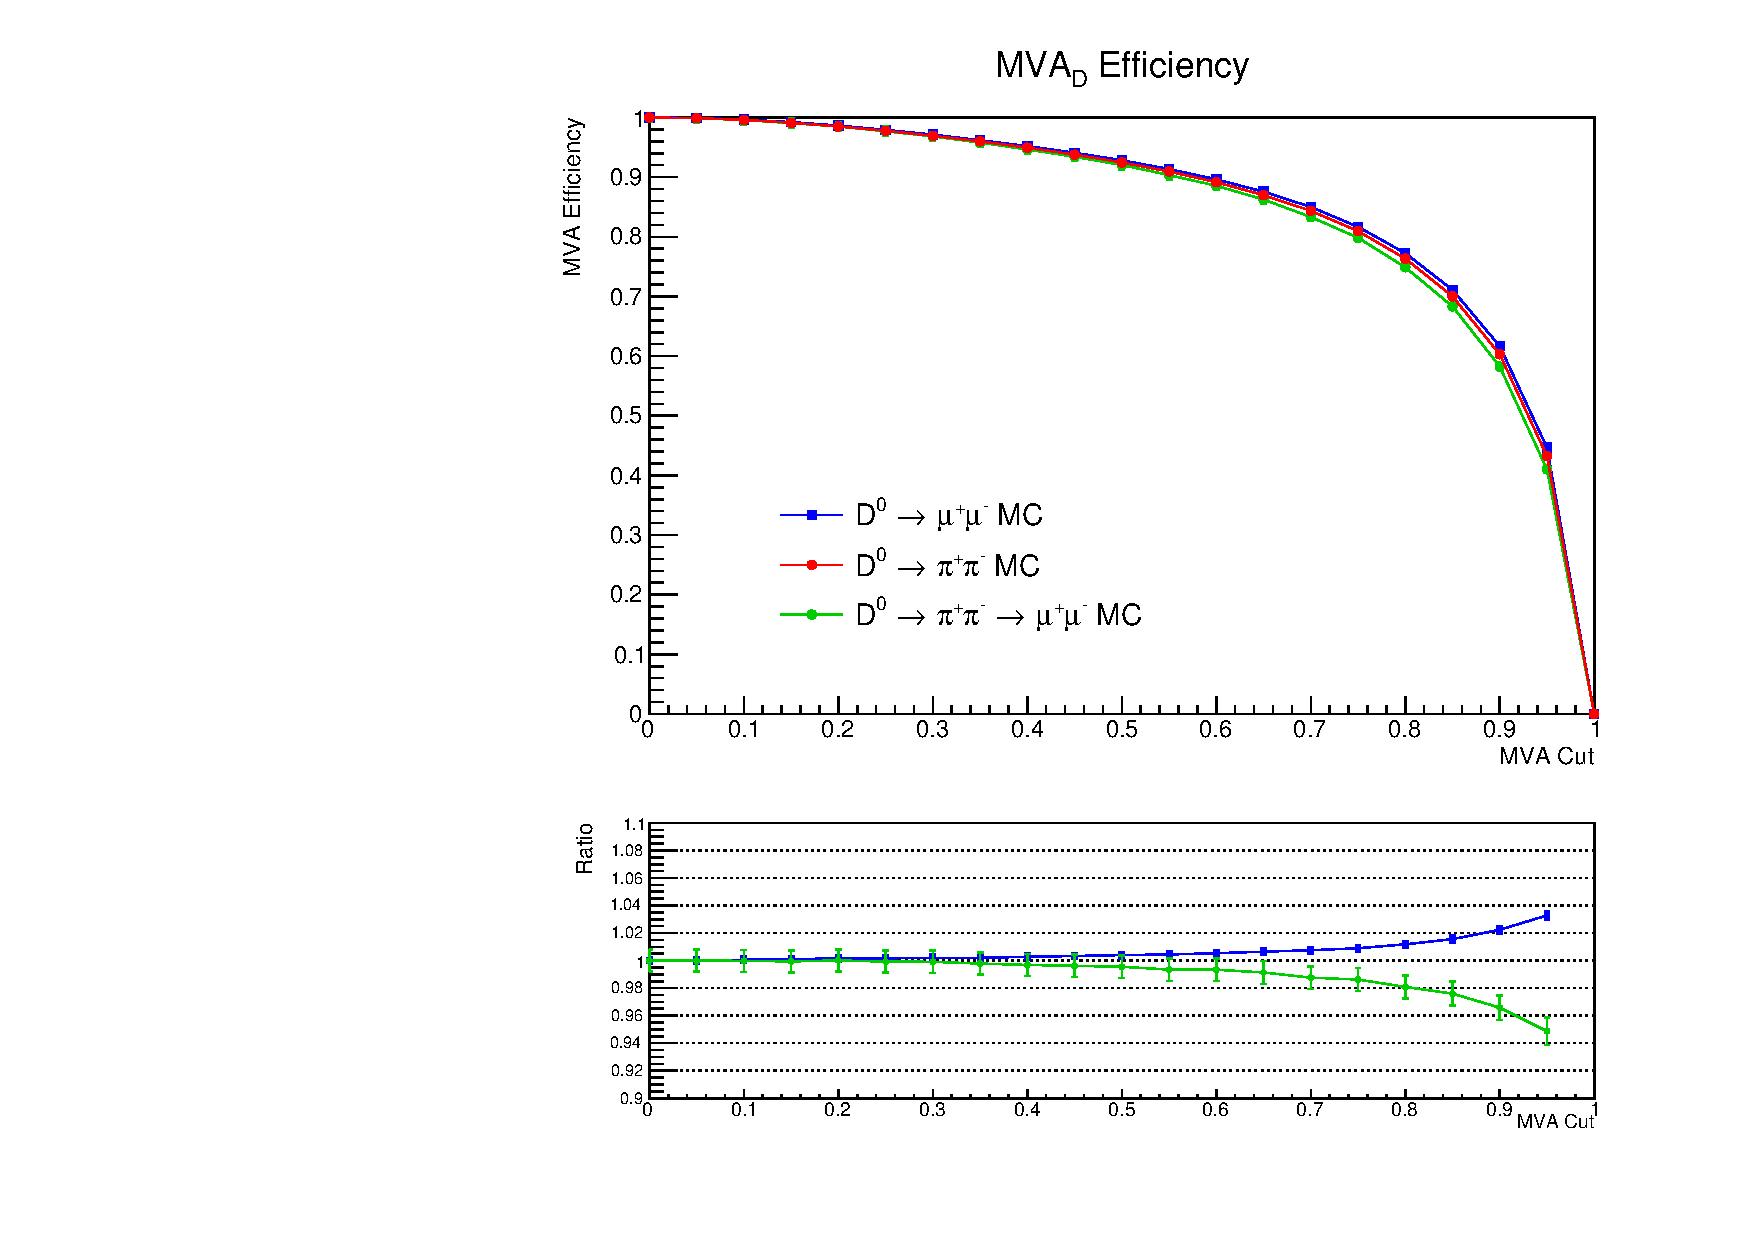
\includegraphics[width=0.5\textwidth]{figures/chapter4/mva/mva_efficiency.pdf}
    \end{center}
    \caption{
      A graphical summary of $\text{MVA}_D$ cut efficiency at various diverse cut values on various samples used throughout the analysis.
    }
    \label{fig:mva_cut_efficiencies}
\end{figure}

As can be seen in table \ref{tab:mva_cut_efficiencies} as well as figure \ref{fig:mva_cut_efficiencies}, while the efficiency values are, as expected, extremely close in the MC samples, there is still a small difference between the three decay channels. To account for this small difference, we calculate a corrective efficiency factor, derived from MC. We name this corrective factor $\text{MVA}_{D, cor}$ and define it as
\begin{equation}
    \begin{split}
    \text{MVA}_{D,\text{cor}\;(D^0 \to \mu^+ \mu^-)} &= 
    \frac{\epsilon_{D^0 \to \mu^+ \mu^-\; \text{ (simulation)}}}
         {\epsilon_{D^0 \to \pi^+ \pi^-\; \text{ (simulation)}}} \\
    \text{MVA}_{D,\text{cor}\;(D^0 \to \pi^+ \pi^- \to \mu^+ \nu_\mu \mu^- \nu_\mu)} &= 
    \frac{\epsilon_{D^0 \to \pi^+ \pi^- \to \mu^+ \nu_\mu \mu^- \nu_\mu\; \text{ (simulation)}}}
         {\epsilon_{D^0 \to \pi^+ \pi^-\; \text{ (simulation)}}}
    \end{split}
\end{equation}
From these definitions, one can extrapolate to data due to the proximity of the efficiency values, meaning
\begin{equation}
    \begin{split}
    \epsilon_{D^0 \to \mu^+ \mu^-} \text{ (data)} &= 
    \epsilon_{D^0 \to \pi^+ \pi^-} \text{ (data)} 
    \times \text{MVA}_{D,\text{cor}\;(D^0 \to \mu^+ \mu^-)} \\
    \epsilon_{D^0 \to \pi^+ \pi^- \to \mu^+ \nu_\mu \mu^- \nu_\mu} \text{ (data)} &= 
    \epsilon_{D^0 \to \pi^+ \pi^-} \text{ (data)} 
    \times \text{MVA}_{D,\text{cor}\;(D^0 \to \pi^+ \pi^- \to \mu^+ \nu_\mu \mu^- \nu_\mu)}
    \end{split}
\end{equation}
Lastly, a very conservative systematic error is assigned to the $\text{MVA}_{D, cor}$ factors of $|1-\text{MVA}_{D, cor}|$. Therefore, we get
\begin{equation}
\begin{split}
    \text{MVA}_{D,\text{cor}\;(D^0 \to \mu^+ \mu^-)} &= 1.009\;\pm\;0.012 \; \text{(stat)}\;\pm\;0.009 \; \text{(sys)} \\
    \text{MVA}_{D,\text{cor}\;(D^0 \to \pi^+ \pi^- \to \mu^+ \nu_\mu \mu^- \nu_\mu)} &= 0.987\;\pm\;0.020 \; \text{(stat)}\;\pm\;0.013 \; \text{(sys)}
\end{split}
\end{equation}
    
\section{Unbinned Maximum Likelihood Fits}
\label{sec:UML}

Now that we have given accurate descriptions of the datasets and selection processes used in this analysis, we are now ready to extract the two main values needed for this analysis, the number of $D^0 \to \pi^+ \pi^-$ events, denoted $N_{D^0 \to \pi^+ \pi^-}$, the number of $D^0 \to \mu^+ \mu^-$ events, denoted $N_{D^0 \to \mu^+ \mu^-}$.

In order to do this, we perform two unbinned maximum likelihood (UML) fits on the events in our data that passes the preselection, baseline selection, and MVA selection processes. Maximum likelihood (ML) fits are statistical methods used to estimate parameters of a model given observed data. A ML fit is a UML fit when the data is not binned into a histogram, but rather the exact data values are used. UML fits define a model $f(\vec{x}; \theta, \theta_N)$, which is a PDF over some set of observed variables, $\vec{x}$ and some model parameters $\theta$ and $\vec{\theta}_N$. The goal of a UML fit is to extract a model parameter $\theta$ given some observed data $\vec{x}_1, \vec{x}_2,...,\vec{x}_N$. $\vec{\theta}_N$ are considered nuisance parameters and are important to defining the model, but are not parameters of interest to the analysis. Once a model has been defined, a likelihood is defined as
\begin{equation}
    \mathcal{L}(\theta, \vec{\theta}_N) = \prod^N_{i=1} f(\vec{x}_i; \theta, \vec{\theta}_N)
\end{equation}
In this formulation, the UML fit can be represented as finding $\hat{\theta} \hat{\vec{\theta}_N}= \text{argmax}_{\theta, \vec{\theta}_N} \mathcal{L}(\theta, \vec{\theta}_N)$\footnote{In practice, this isn't quite true. Often in applications with lots of nuisance parameters, UML fits operate using profile likelihoods. However, the point of this discussion is merely an overview of UML and the complexities will be ignored.}. 

In our analysis, $\theta$ is the true number of signal events (in the normalization channel this is $N_{D^0 \to \pi^+ \pi^-}$ and in our signal channel this is $N_{D^0 \to \mu^+ \mu^-}$), $\vec{x}$ is the $\Delta m$ and $m(D^0)$ of our data, and $\vec{\theta}_N$ are the variance parameters needed to construct the signal and background PDFs. As can be seen in figure \ref{fig:mva_correlation_matrix_for_fit_variables}, there exists practically no correlation between $\Delta m$ and $m(D^0)$. This tells us that the 2D model can be split as a product of 1D models. More specifically, we have that
\begin{equation}
    f(\vec{x}; \theta, \theta_N) = f_{m(D^0)}(m(D^0); \theta, \theta_N) \times f_{\Delta m}(\Delta m; \theta, \theta_N)
\end{equation}

A more precise discussion of this construction follows in the sections below. For each of the two channels we begin by developing the models for both the signal and the background. Then, we outline the specifics of the fit and any corrections applied to it. Lastly, we outline the results of the fit. 

\subsection{Normalization Channel Fit}
\label{subsec:normalization_channel_fit}

The goal of the normalization channel is to extract $N_{D^0 \to \pi^+ \pi^-}$. This is done using the \texttt{HLT\_ZeroBias} trigger dataset, as is described in section \ref{subsec:data_samples}. Perhaps the largest difficulty of the UML fit on the normalization channel is that the \texttt{HLT\_ZeroBias} trigger dataset does not contain many of the $D^{*\pm}\to D^0 \pi^\pm, D^0 \to \pi^+ \pi^-$ signal events due the large prescaling factor of the trigger, discussed in section \ref{subsec:data_samples}. The below section, in part, describes in detail how this difficulty is overcome by using MC samples to inform the fit and correcting for MC mismodeling effects when needed in the final fit. 

\subsubsection{Signal Model}

The signal model for the normalization channel describes the $\Delta m$ and $m(D^0)$ of the $D^{*\pm}\to D^0 \pi^\pm, D^0 \to \pi^+ \pi^-$ decay. As is common to do for masses in signal distributions, the model for $m(D^0)$ is a sum of two Gaussian distributions forced to share a common mean. Similarly, the model for $\Delta m$ is a sum of three Gaussian distributions forced to share a common mean.

Due to the small number of signal events in data, the shape (composing of the means and standard deviations) of this model is determined by fits to simulated MC samples. This is because the shape will be much more stable in MC compared to data, simply just because there are more samples in MC. Once the shape is found using MC, it is frozen and only the number of events is allowed to float when the fit is applied to data. The signal model fit to MC can be seen in figure \ref{fig:d0pipi_uml_fit_pipi_model}.

\begin{figure}[htp]
    \begin{center}
      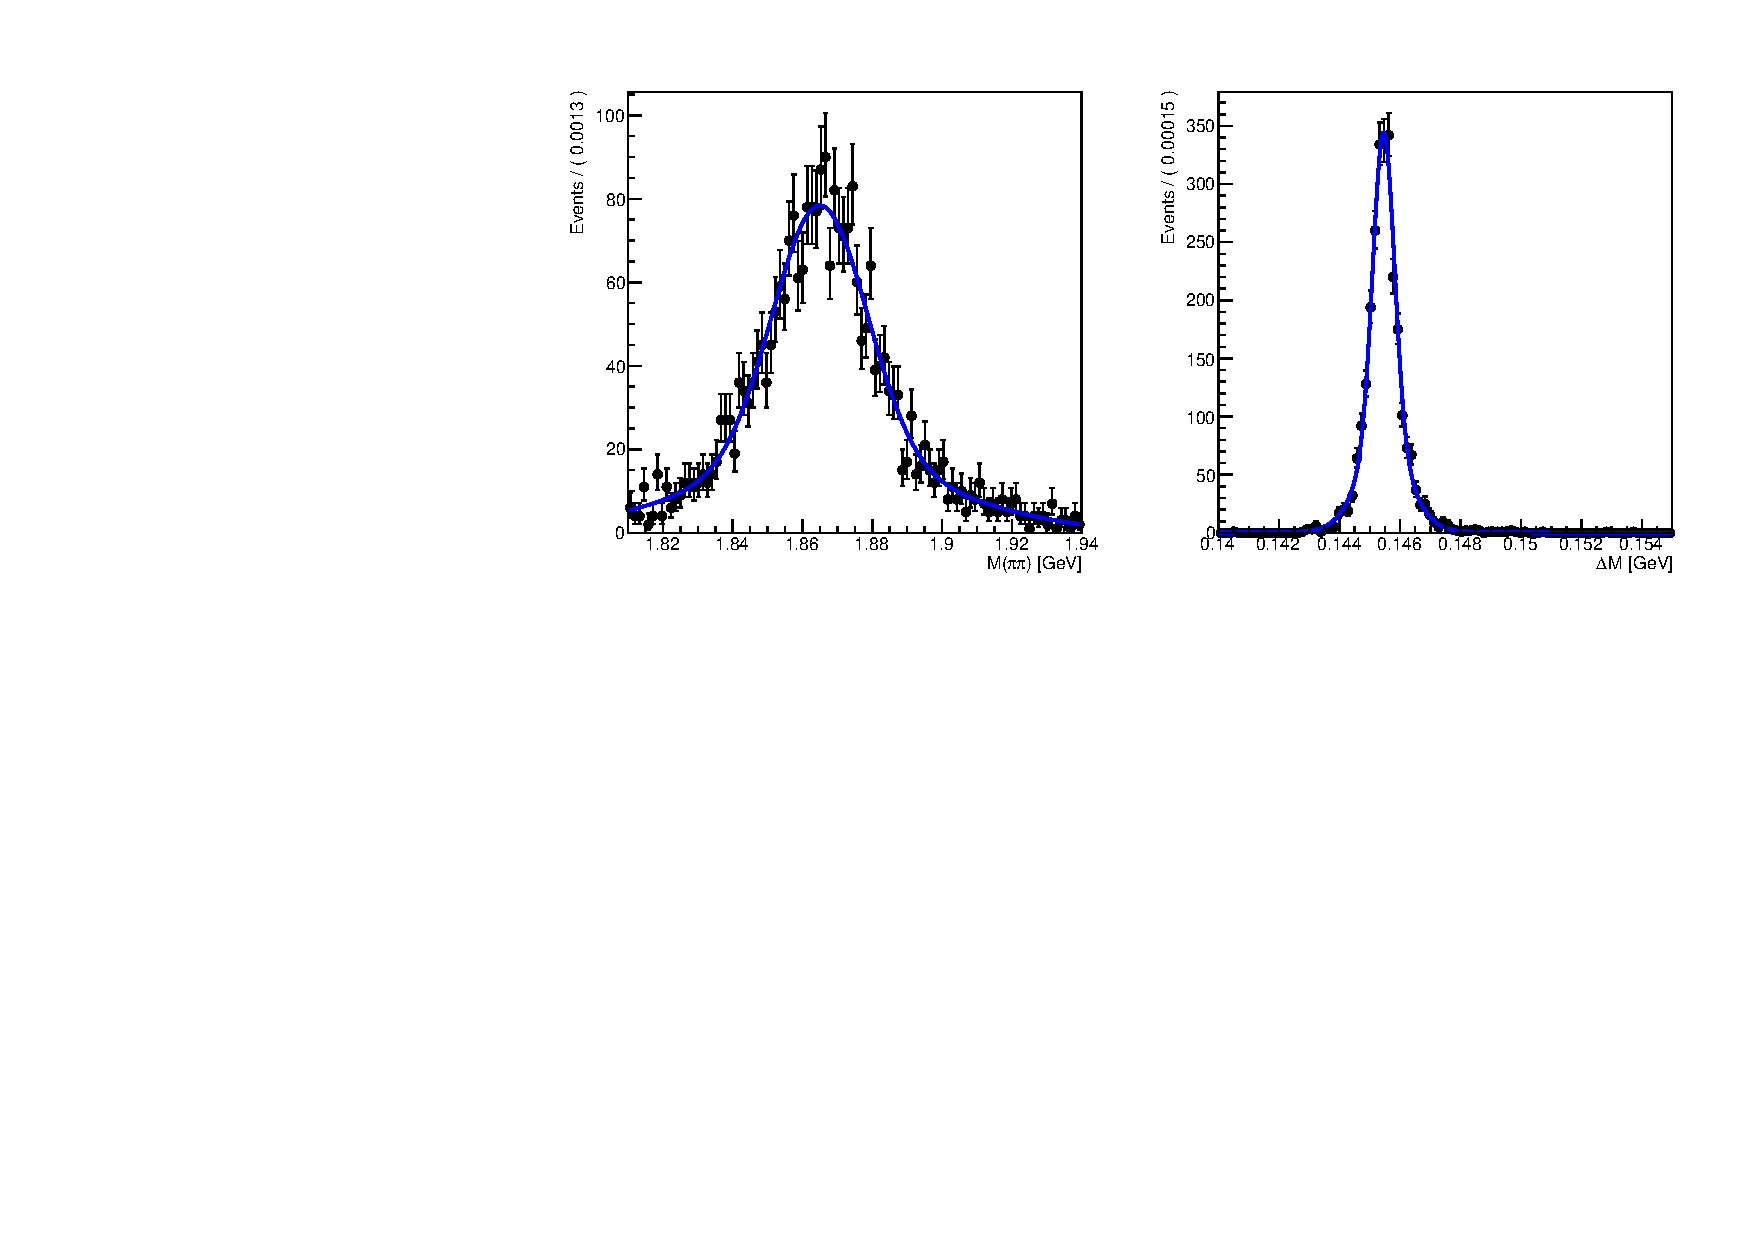
\includegraphics[width=0.9\textwidth]{figures/chapter4/normalization_fit/dpipi_fit_mc.pdf}
    \end{center}
    \caption{
      The signal model fit on MC samples, with $m(D^0)$ displayed left and $\Delta m$ displayed right.
    }
    \label{fig:d0pipi_uml_fit_pipi_model}
\end{figure}

It is possible, however, that the shape varies slightly between the MC samples and data, due to mismodeling in MC. To account for this slight mismodeling affect, we derive correction factors $\mu_{\text{corr}}$ and $\sigma_{\text{corr}}$ such that
\begin{equation}
\begin{split}
    \mu_{\text{data}} &= \mu_{\text{MC}} \times (1+\mu_{\text{corr}}) \\
    \sigma^i_{\text{data}} &= \sigma_{\text{MC}} \times (1+\sigma_{\text{corr}}) 
\end{split}
\label{eq:shape_correction_definition}
\end{equation}
where $i$ is used to denote that each of the models has multiple width parameters (one for each Gaussian distribution that is summed) but only one mean parameter.

To derive what this correction factor is, we use the \texttt{HLT\_DoubleMu4\_3\_LowMass} trigger to construct a dataset with enough signal samples to construct a reliable data-driven fit shape. We then run the full normalization channel UML fit (including the background models) on this data. Comparing that to the shape obtained from MC, we can easily derive the $\mu_{\text{corr}}$ from equation \ref{eq:shape_correction_definition}. 

Initially, it might seem that one could apply the same procedure to find $\sigma_{\text{corr}}$. However, this dimuon trigger enhances the amount of $b\bar{b}$ production in the sample, which biases the width of the $D^{*\pm}\to D^0 \pi^\pm, D^0 \to \pi^+ \pi^-$ decay. Therefore, one must first properly understand that bias before applying the correction in the same way as the mass was done. To understand the bias effect between the Dimuon and Zerobias triggers, we compare $D^{*\pm}\to D^0 \pi^\pm, D^0 \to K^\pm \pi^\mp$ fits from the Dimuon and Zerobias dataset. This is possible because the Kaon decay mode is much more frequent than the pion decay mode. The fitting process is the same as before and the width correction 
can be obtained as
\begin{equation}
    \begin{split}
        1+\sigma_{\text{corr}} &= \left(1+\sigma_{\text{corr, DoubleMuon}}^{D^0\to\pi^+\pi^-}\right) \\
        &\times \frac{
            1+\sigma_{\text{corr, ZeroBias}}^{D^0\to\pi^\pm\pi^\mp}
        }{
            1+\sigma_{\text{corr, DoubleMuon}}^{D^0\to K^\pm\pi^\mp}
        }
    \end{split}
\end{equation}    
%All of the corrections to the signal shape are summarized TODO: add table reference.

%TODO: add table of width corrections.  Likely won't do this

\subsubsection{Background Model}

As described in section \ref{subsec:backgrounds}, there are 3 peaking backgrounds and a combinatorial background to consider in the normalization channel. 

To begin, we describe the 3 peaking backgrounds. The first, as most prominent, of these three backgrounds is the $D^{*\pm} \to D^0\pi^\pm, D^0 \to K^\pm \pi^\mp$. As shown in figure \ref{fig:reconstructed_D0_comparison}, the $m(D^0)$ peak is shifted significantly to the left due to incorrect mass of the pion imposed on the kaon during reconstruction. In fact, the mean in shifted so far that only the tail of the Gaussian distribution persists in the mass region of our fit. Since the tail of a Gaussian distribution is approximately an exponential function, we use an exponential function to fit the $m(D^0)$ parameter. This fit proves to be significantly more stable as the exponential function only has one shape parameter that requires fitting while the Gaussian distribution has two. In contrast, the $\Delta m$ distribution of the $D^{*\pm} \to D^0\pi^\pm, D^0 \to K^\pm \pi^\mp$ decay closely follows the shape of the signal. Therefore, we similarly use a sum of three Gaussian distributions with a common mean do model the $\Delta m$ distribution. The convergence of the fit is verified using MC samples and is displayed in figure \ref{fig:d0pipi_uml_fit_kpi_model}. The data fit remains stable even when these shape parameters are allowed to vary. Therefore, we allow the shape of this peaking background to vary when fit to data. 

\begin{figure}[htp]
    \begin{center}
      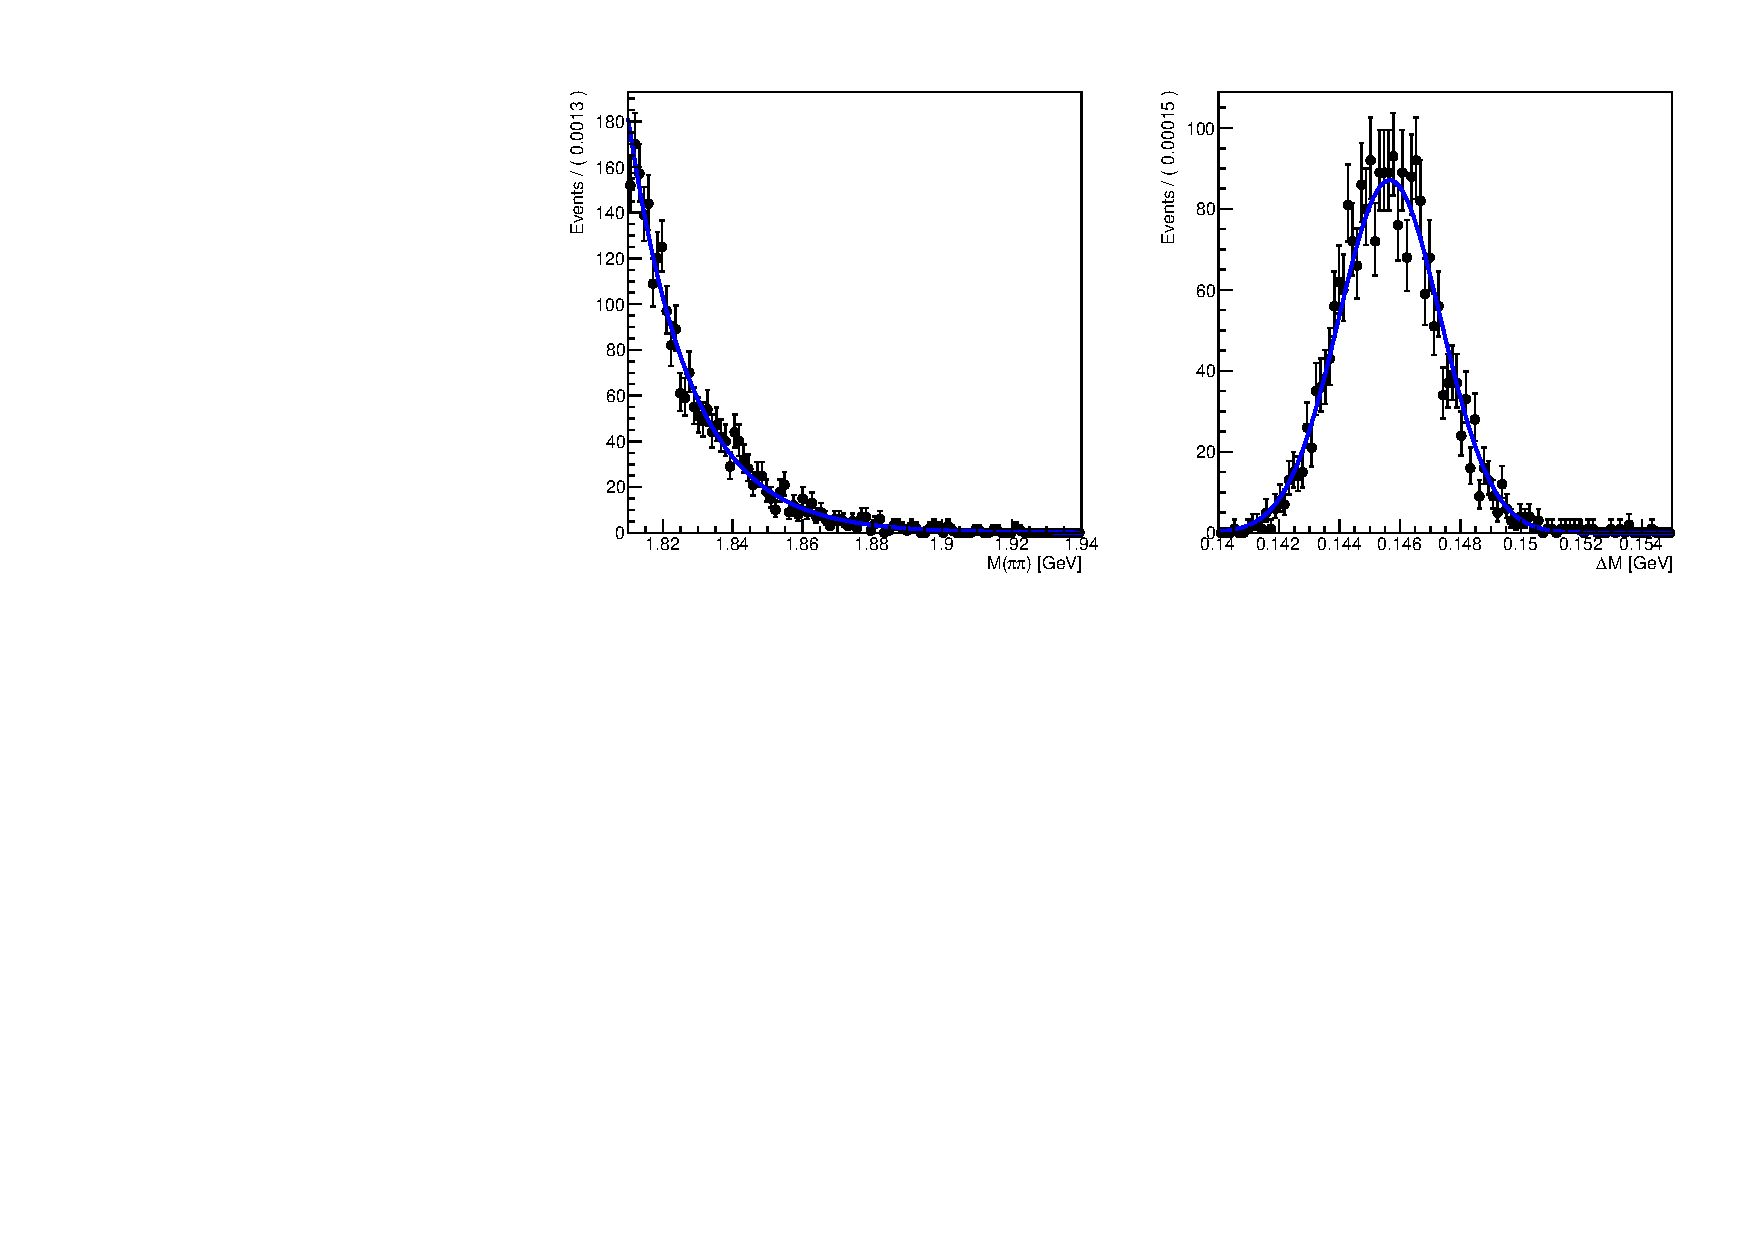
\includegraphics[width=0.9\textwidth]{figures/chapter4/normalization_fit/dpipi_fit_mc_kpi.pdf}
    \end{center}
    \caption{
      The $D^{*\pm} \to D^0\pi^\pm, D^0 \to K^\pm \pi^\mp$ model fit on MC samples, with $m(D^0)$ displayed left and $\Delta m$ displayed right.
    }
    \label{fig:d0pipi_uml_fit_kpi_model}
\end{figure}

The other two peaking backgrounds correspond to $D^0 \to \mu^+ \mu^-$ and $D^0 \to K^\pm \pi^\mp$ decays where the $D^0$ meson does not originate from a $D^*$ meson. Importantly, these have the same $m(D^0)$ shape as their $D^{*\pm} \to D^0 \pi^\pm$ counterparts, so the shape derived from their counterparts is copied exactly into their models. The $\Delta m$ of these decays, however, does not represent a peak but rather a combinatorial signature. This is due to the combinatorial nature of the production mechanisms of the $D^0$ meson that pass the selection criterion. Therefore, we fit a combinatorial background model for the $\Delta m$ values of both non-$D^{*\pm} \to D^0 \pi^\pm$ decays. 

The combinatorial background for $m(D^0)$ is an exponential function, as is common for modeling combinatorial backgrounds of reconstructed rest masses. The combinatorial background for $\Delta m$, however, has more complex shape than just an exponential. In this work, we use the $\texttt{RooDstD0Bg}$ function \cite{ref:verkerke2003roofit} given by
\begin{equation}
    P(m|m_0, A, B, C) = \left(1 - \exp \left(-\frac{m-m_0}{C} \right) \right) \left( \frac{m}{m_0}\right)^A
\end{equation}
The shape of these functions is derived from fits to the data side-band regions where the distance from the signal resonance guarantees virtually no peaking background contribution. This shape is frozen to allow for fit stability when the model is used in the final data fit. Figure \ref{fig:d0pipi_uml_fit_comb_model} shows the convergence of the shape on the data side-bands.

\begin{figure}[htp]
    \begin{center}
      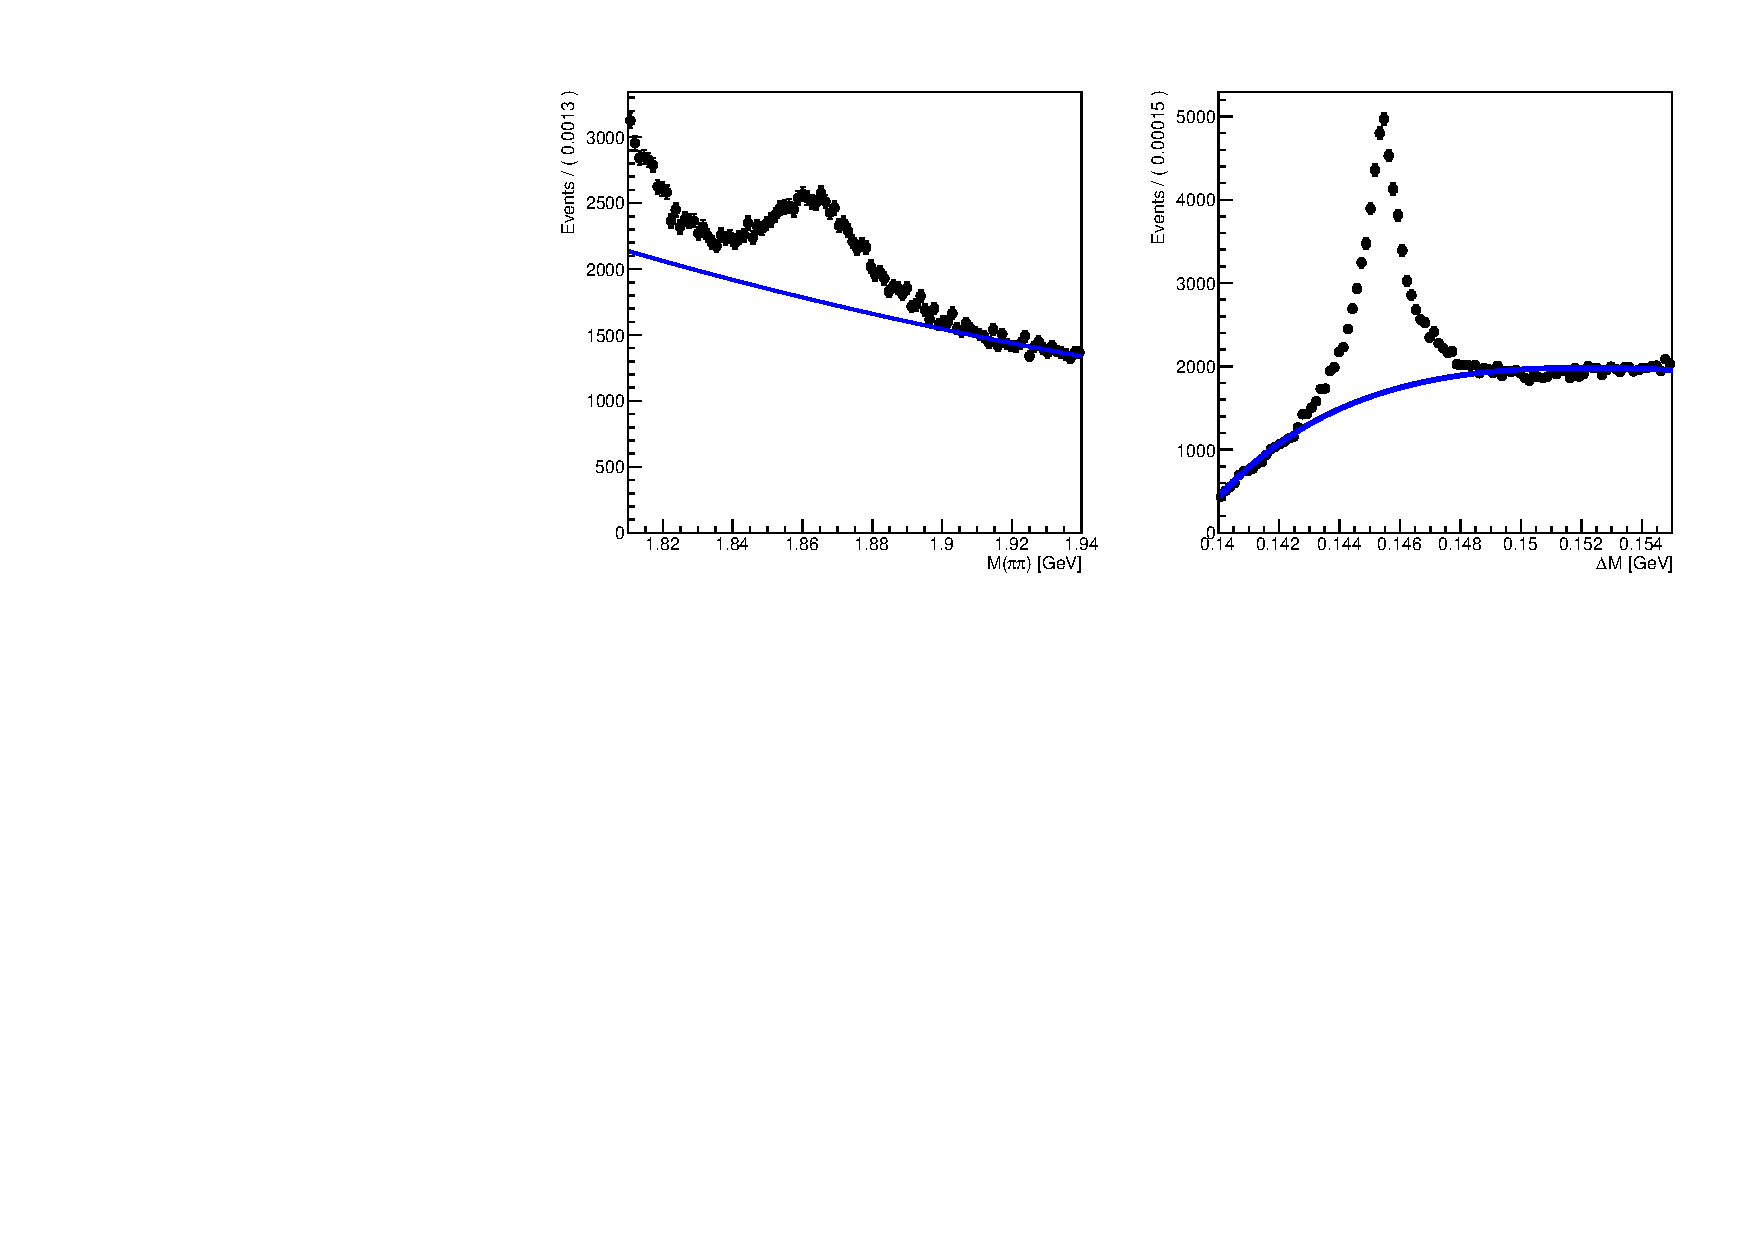
\includegraphics[width=0.9\textwidth]{figures/chapter4/normalization_fit/dpipi_fit_comb.pdf}
    \end{center}
    \caption{
      The combinatorial model fit on data side-bands, with $m(D^0)$ displayed left and $\Delta m$ displayed right.
    }
    \label{fig:d0pipi_uml_fit_comb_model}
\end{figure}

\subsubsection{Fit Results}

The final model used for the fit is a sum of signal model and all the background models. We check the convergence of this model on the \texttt{HLT\_DoubleMu4\_3\_LowMass} data, which contains significantly more signal events than the \texttt{HLT\_ZeroBias} trigger samples, allowing us to visually inspect the stability of the fit, as is seen in figure \ref{fig:d0pipi_uml_fit_dimuon} and table \ref{tab:d0pipi_uml_fit_results}. Importantly, the $D^0 \to K^\pm \pi^\mp$ decays where the $D^0$ meson does not originate from a $D^*$ meson contibutes virtually no events to the fit. Therefore, to increase the stability of the fit, we force the integral under this the non-$D^*,D^0 \to K^\pm \pi^\mp$ model to 0. 

Finally, the fit is applied to the \texttt{HLT\_ZeroBias} trigger samples. A graphical representation of the fit can be seen in figure \ref{fig:d0pipi_uml_fit} and the results are summarized in table \ref{tab:d0pipi_uml_fit_results}.


\begin{figure}[htp]
    \begin{center}
      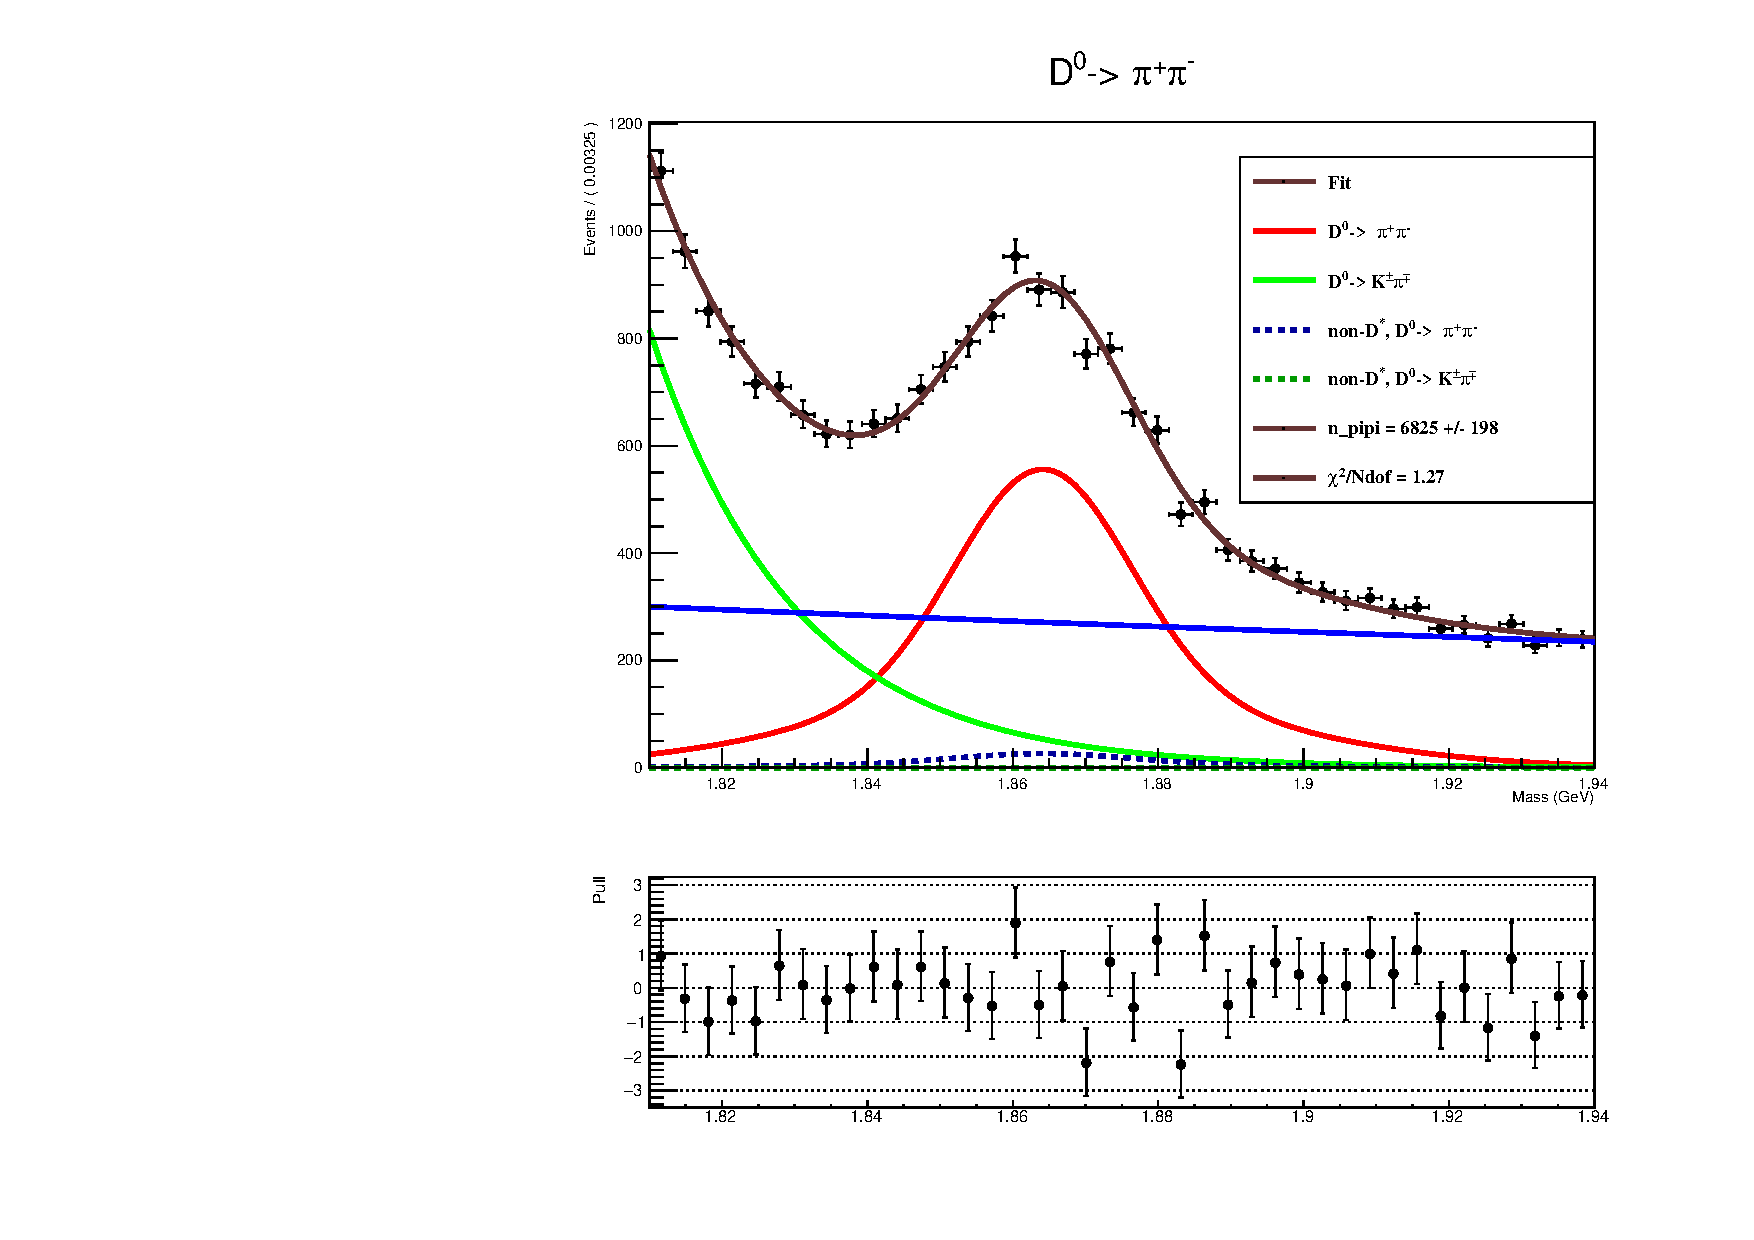
\includegraphics[width=0.45\textwidth]{figures/chapter4/normalization_fit/m_pipiDimuon_afterMvaCut.pdf}
      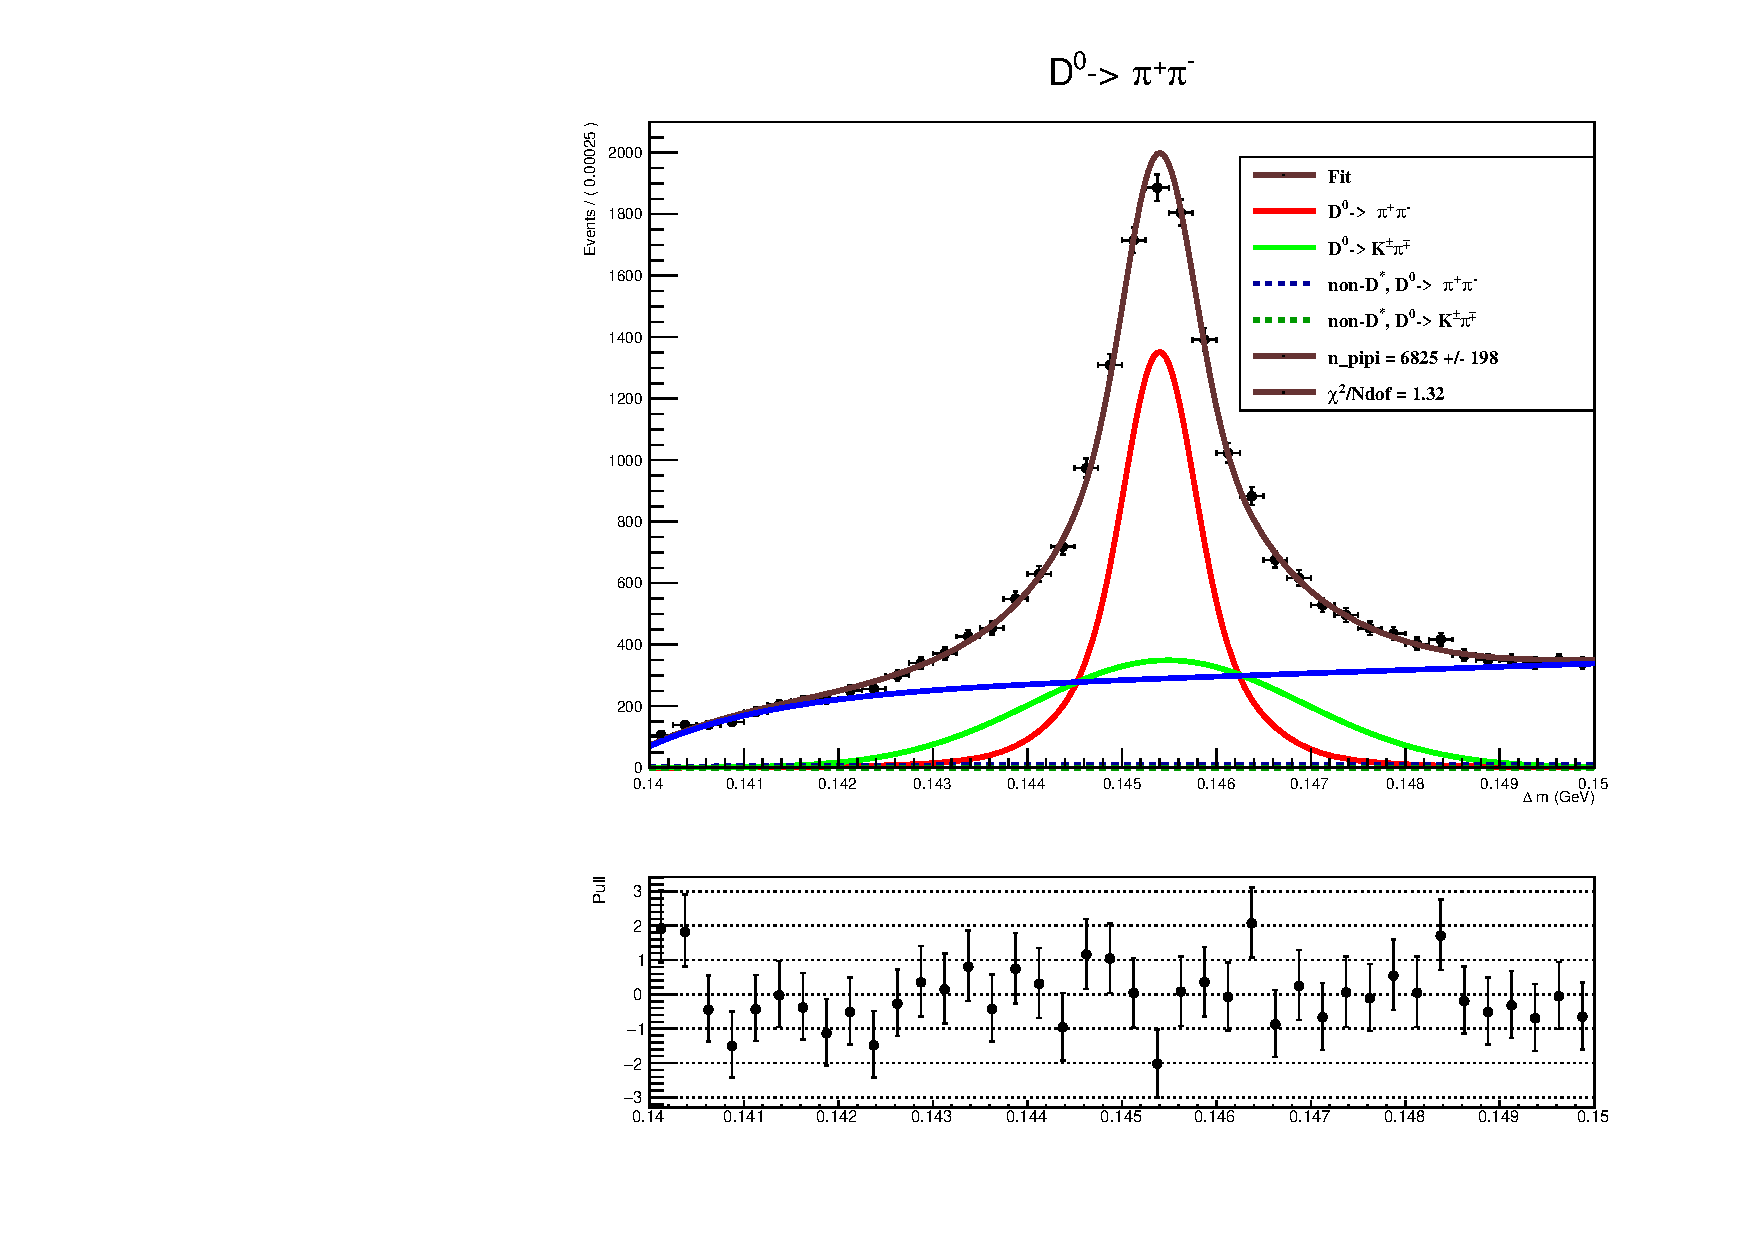
\includegraphics[width=0.45\textwidth]{figures/chapter4/normalization_fit/dm_pipiDimuon_afterMvaCut.pdf}\\
    \end{center}
    \caption{
        The full $D^0 \to \pi^+ \pi^-$ model fit on \texttt{HLT\_ZeroBias} data, with $m(D^0)$ displayed left and $\Delta m$ displayed right.
    }
    \label{fig:d0pipi_uml_fit}
\end{figure}

\begin{figure}[htp]
    \begin{center}
      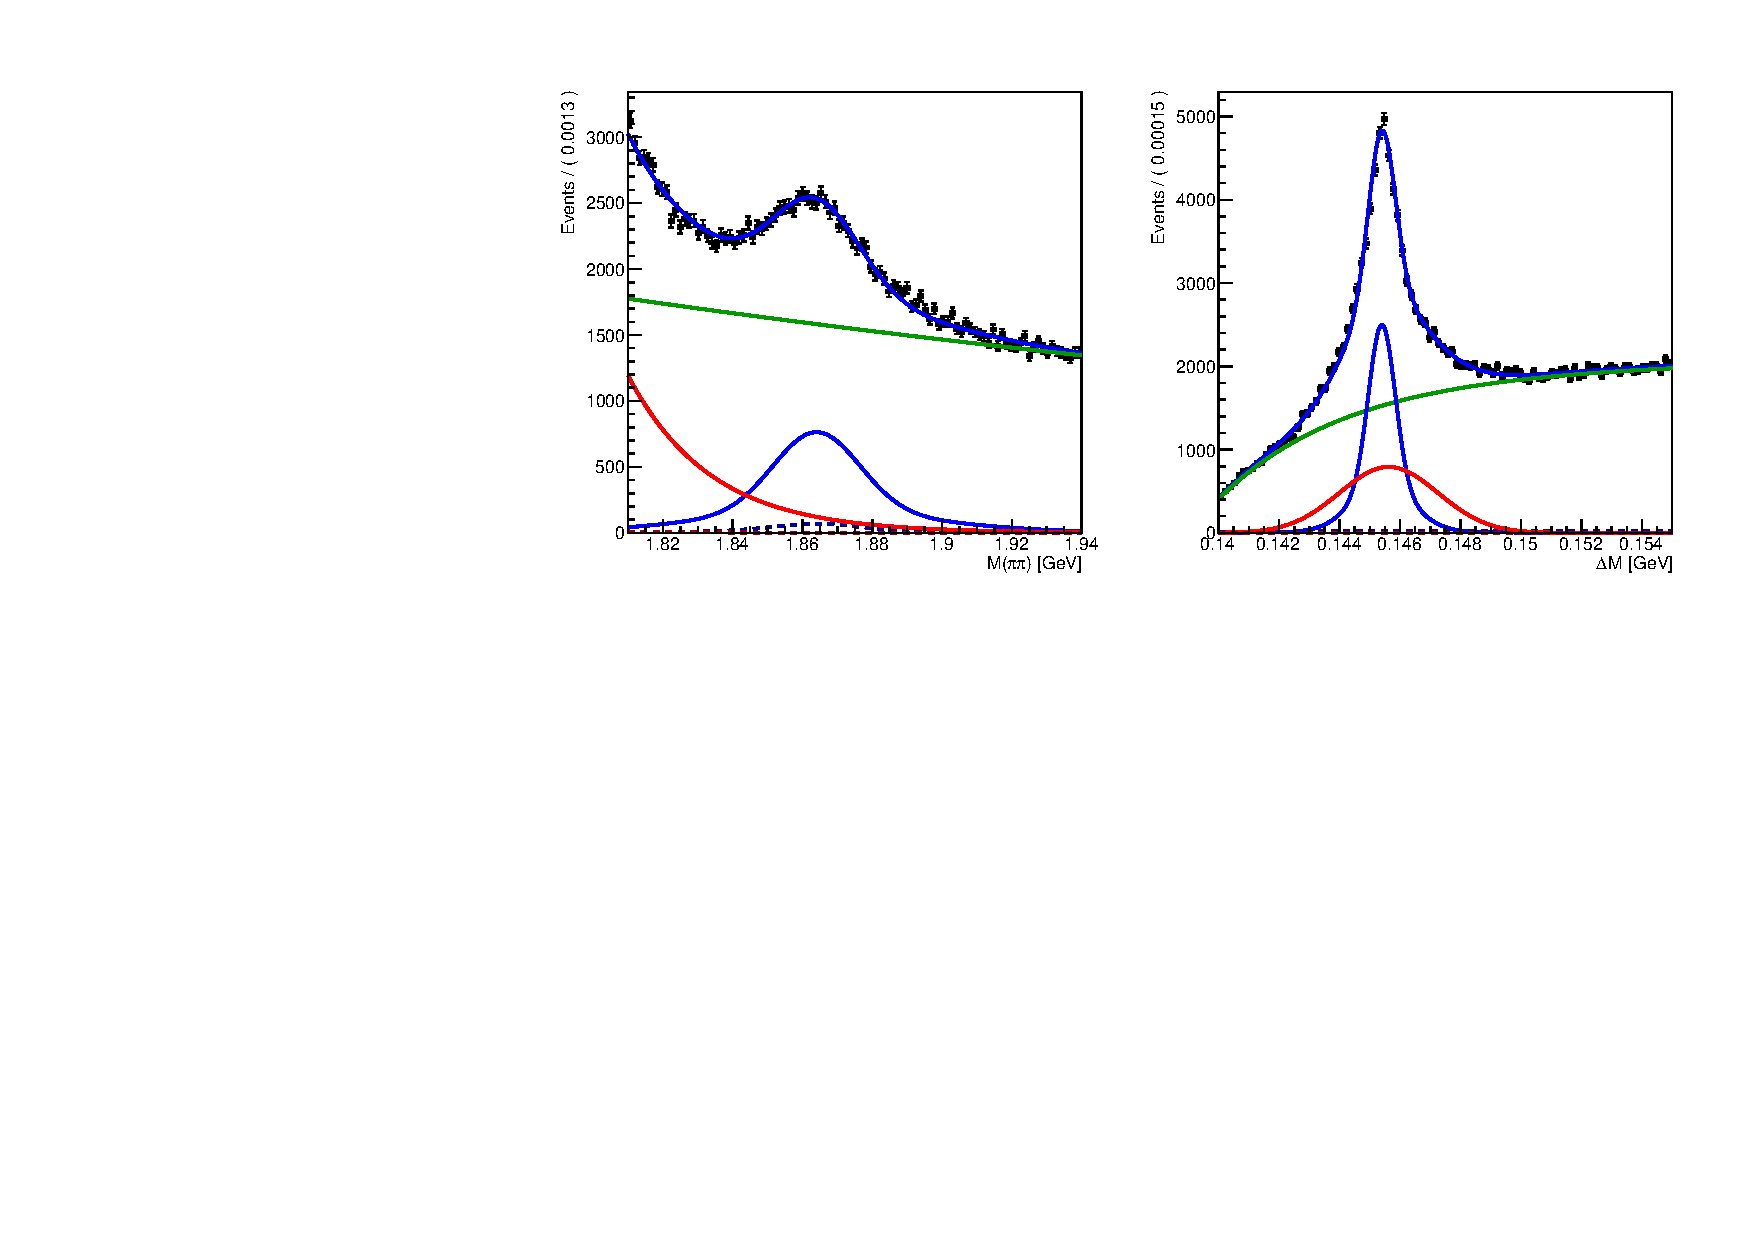
\includegraphics[width=0.9\textwidth]{figures/chapter4/normalization_fit/dpipi_fit.pdf}
    \end{center}
    \caption{
      The full $D^0 \to \pi^+ \pi^-$ model fit on \texttt{HLT\_DoubleMu4\_3\_LowMass} data, with $m(D^0)$ displayed left and $\Delta m$ displayed right. The green line follows the combinatorial model, the blue line follows the signal model, the red line follows the $D^{*\pm} \to D^0\pi^\pm, D^0 \to K^\pm \pi^\mp$ background model, the red dashed line following the non-$D^{*\pm} \to D^0\pi^\pm, D^0 \to K^\pm \pi^\mp$ background model, and the blue dashed line follows the non-$D^{*\pm} \to D^0\pi^\pm, D^0 \to \pi^+ \pi^-$ background model.
    }
    \label{fig:d0pipi_uml_fit_dimuon}
\end{figure}


\begin{table}[h!]
    \centering
    \begin{tabular}{@{}lrr@{}}
    \toprule
    \toprule
    \textbf{\texttt{HLT\_DoubleMu4\_3\_LowMass} data}& Fitted count & Fitted error  \\
    \midrule
    $D^*, D^0 \to \pi\pi$ Yield        & 23787 & $\pm$509 \\
    $D^*, D^0 \to K\pi$ Yield          & 21558  & $\pm$749 \\
    Combinatorial Yield               & 155088 & $\pm$1722 \\
    non--$D^*$, $D^0 \to \pi\pi$ Yield & 2140   & $\pm$685 \\
    non--$D^*$, $D^0 \to K\pi$ Yield   & 181     & $\pm$1410 \\
    \bottomrule
    \toprule
    \textbf{\texttt{HLT\_ZeroBias} data} & Fitted count & Fitted error \\
    \midrule
    $D^*, D^0 \to \pi\pi$ Yield        & 195 & $\pm$17 \\
    $D^*, D^0 \to K\pi$ Yield          & 74  & $\pm$21 \\
    Combinatorial Yield               & 140 & $\pm$20 \\
    non--$D^*$, $D^0 \to \pi\pi$ Yield & 0   & $\pm$11 \\
    non--$D^*$, $D^0 \to K\pi$ Yield   & 0     & $\pm$0 \\
    \bottomrule
    \bottomrule
    \end{tabular}
    \caption{Fitted yields and associated uncertainties for the normalization UML fit.}
    \label{tab:d0pipi_uml_fit_results}
    \end{table}

\subsection{Signal Channel Fit}
\label{subsec:signal_channel_uml}

The goal of the signal channel is to extract $N_{D^0 \to \mu^+ \mu^-}$. This is done using the \texttt{HLT\_DoubleMu4\_3\_LowMass} trigger dataset, as is described in section \ref{subsec:backgrounds}. As with the normalization channel, the largest difficult of this UML fit is the lack of signal events due to the small branching fraction of the $D^0$ meson. Similarly to the normalization channel, the signal channel uses MC samples to inform the shapes for data, applying corrections when needed. Additionally, the results of the normalization channel are used to fix the background yields. These techniques are described in the remaineder of the section.

It is worth mentioning that much of the machinery needed for this fit has been developed in section \ref{subsec:normalization_channel_fit} and is therefore not repeated here. Namely, this section focuses on the differences in the signal channel that require special attention.

\subsubsection{Signal Model}

The signal model for the normalization channel describes the $\Delta m$ and $m(D^0)$ of the $D^{*\pm}\to D^0 \pi^\pm, D^0 \to \pi^+ \pi^-$ decay. The same procedure for determining the normalization channel signal model is used in determining this signal model, with the mean and width corrections derived from the normalization channel.

The signal model fit to MC can be seen in figure \ref{fig:d0mumu_uml_fit}.

\begin{figure}[htp]
    \begin{center}
      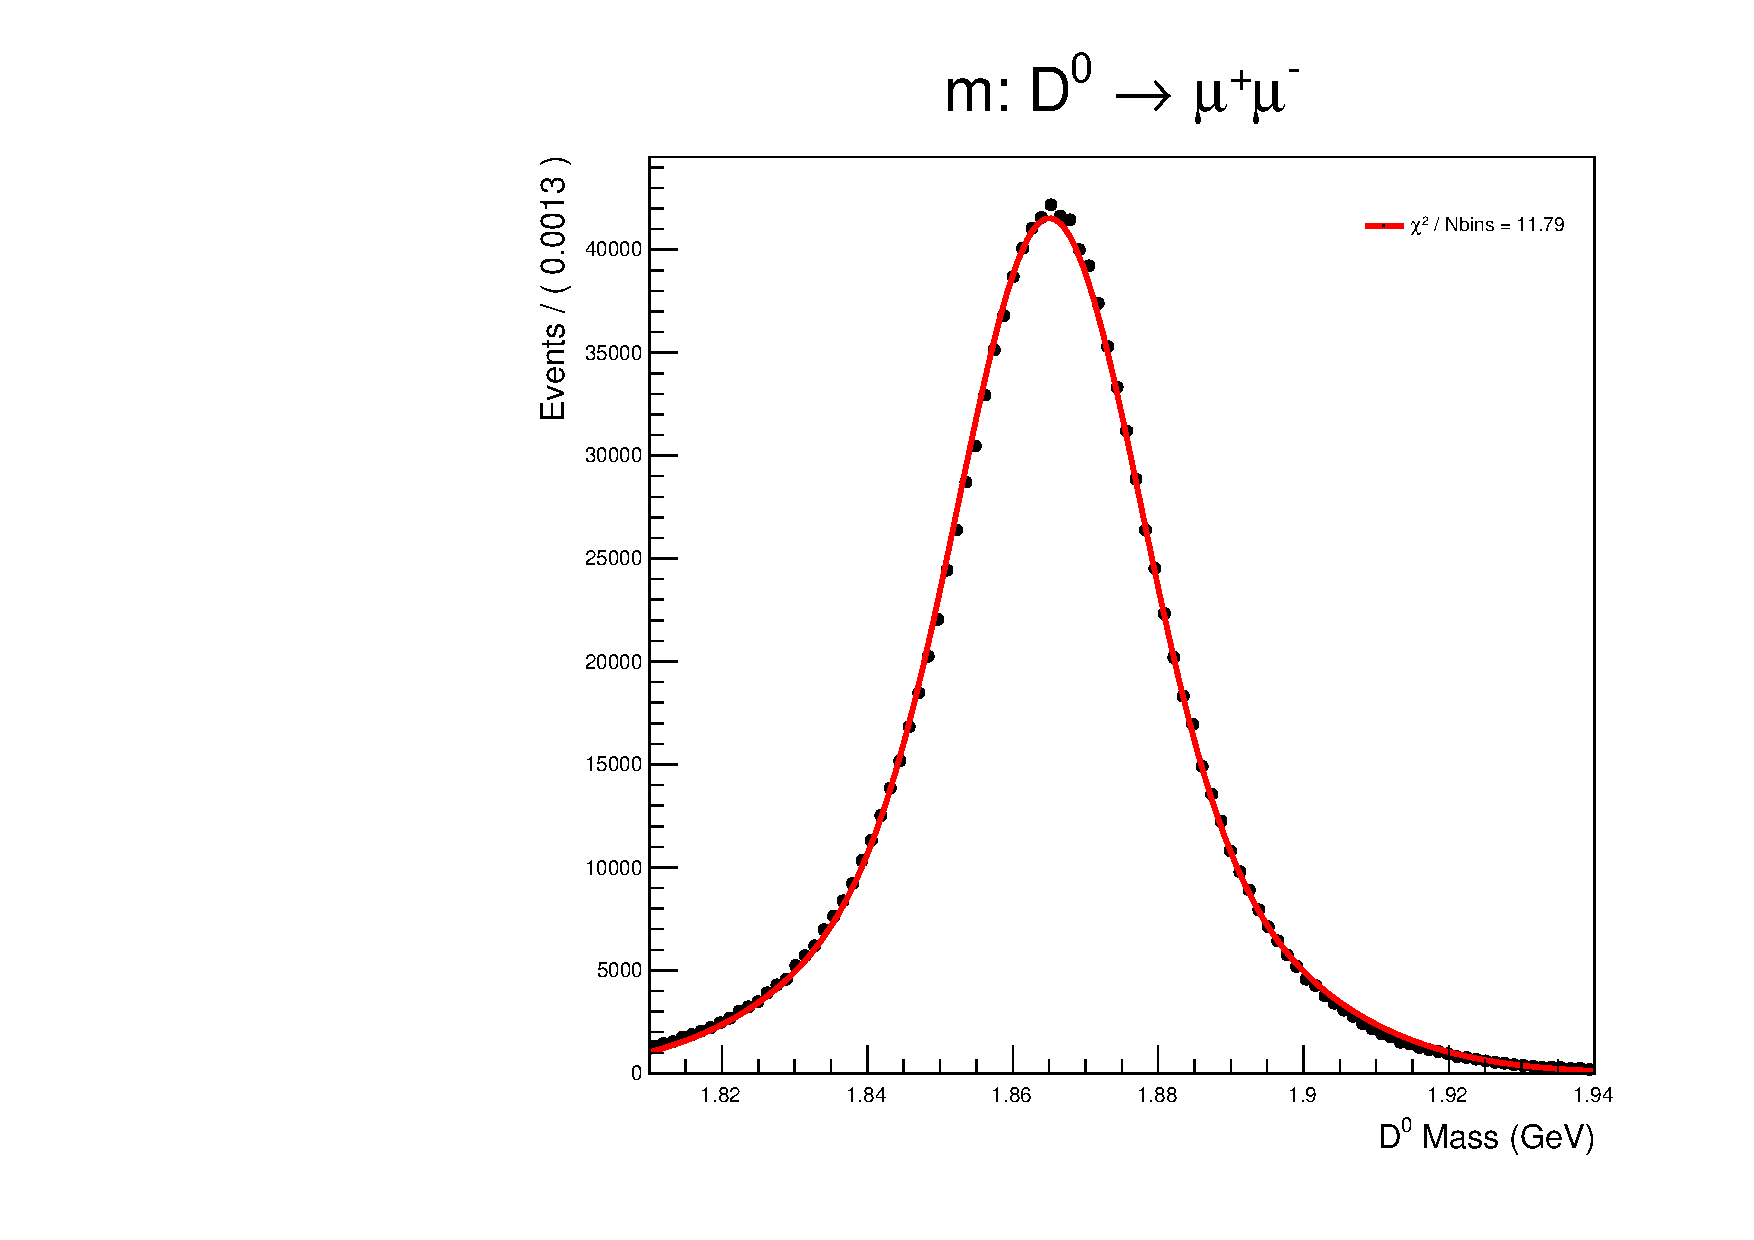
\includegraphics[width=0.45\textwidth]{figures/chapter4/signal_fit/d0mm_2022_2023_0_m.pdf}
      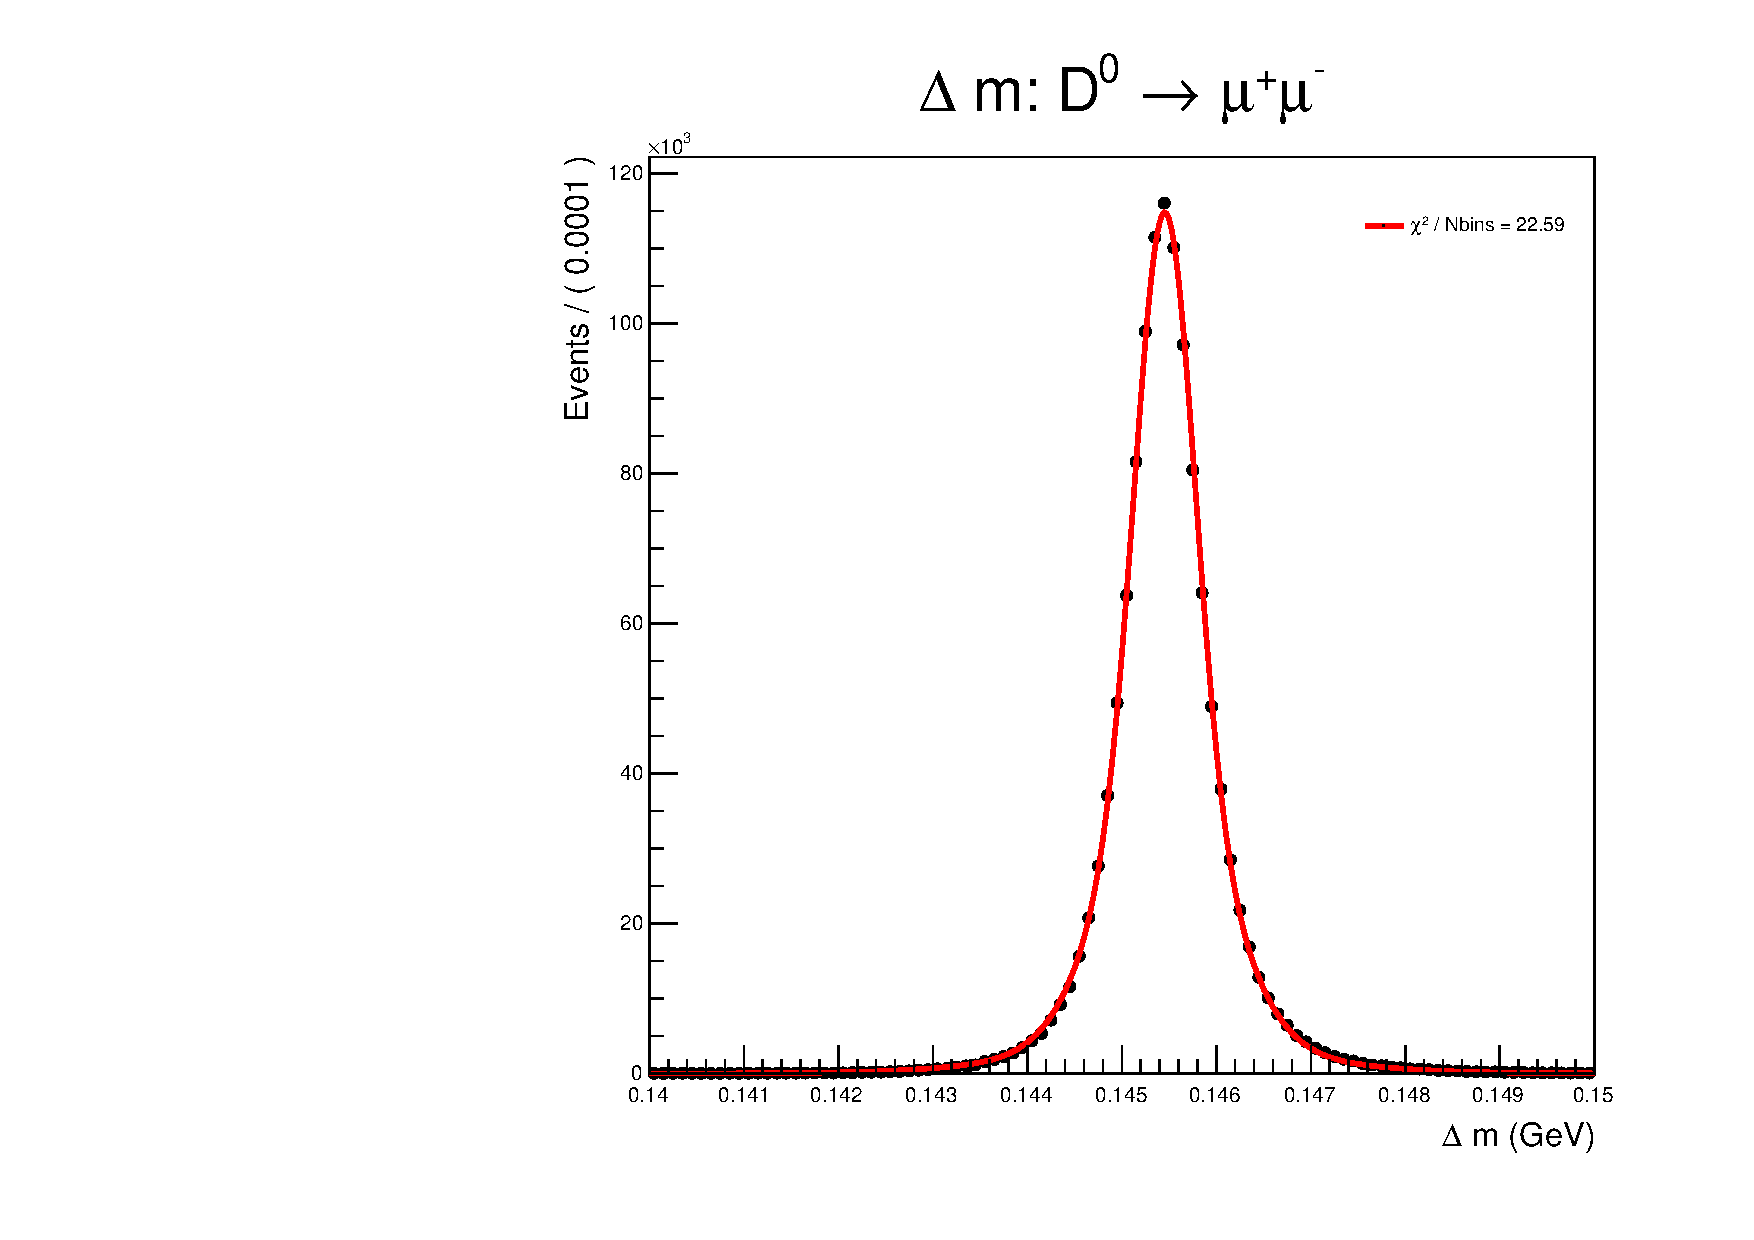
\includegraphics[width=0.45\textwidth]{figures/chapter4/signal_fit/d0mm_2022_2023_0_dm.pdf}\\
    \end{center}
    \caption{
      The signal model fit on MC samples, with $m(D^0)$ displayed left and $\Delta m$ displayed right.
    }
    \label{fig:d0mumu_uml_fit}
\end{figure}

\subsubsection{Background Model}

As is evident from section \ref{subsec:backgrounds}, there are 2 $D^{*\pm} \to D^0 \pi^\pm$ peaking backgrounds and a combinatorial background to consider in the normalization channel. Note that the non-$D^{*\pm} \to D^0 \pi^\pm$ backgrounds which were discussed extensively in the normalization channel are not relevant here due to the large uncertainty of the combinatorial background compared to the expected yield from these backgrounds. Therefore, any non-$D^{*\pm} \to D^0 \pi^\pm$ backgrounds are considered combinatorial and considered in the combinatorial model.

The two peaking backgrounds are $D^{*\pm} \to D^0 \pi^\pm$ processes where the $D^0$ decays via either $D^0 \to \pi^+ \pi^- \to \mu^+ \nu_\mu \mu^- \bar{\nu}_\mu$ (hadronic mode) or via $D^0 \to \pi^- \mu^+ \nu_\mu$ (semileptonic mode). Both of these models are developed using the same process as the signal mode. Namely, the models are built out of sums of Gaussian distributions\footnote{Just like in the signal, two Gaussian distributions sharing a common mean are used for $m(D^0)$ and three Gaussian distributions sharing a common mean are used for $\Delta m$}, their shape is determined by fitting to MC samples, and their means and widths are corrected for using the correction derived in the normalization channel fit. 

In the normalization channel, the yields of these models were left floating. In this channel, there are so few events that allowing for this would destabilize the fit. However, we have already calculated $N_{D^0 \to \pi^+ \pi^-} = 195 \pm 17$ in section \ref{subsec:normalization_channel_fit} and the branching fractions of $\mathcal{B}(D^0 \to \pi^+ \pi^-) = (1.454 \pm 0.024) \times 10^{-3}$ and $\mathcal{B}(D^0 \to \pi^-\mu^+ \nu_\mu) = (2.67 \pm 0.12) \times 10^{-3}$ are well known \cite{ref:pdg2024}. Lastly, in section \ref{sec:muon_fake_rate}, we calculate the fake rate, $f_{\pi \to \mu}$, or the rate at which pions decay to muons in the detector, which occurs once in the semi-leptonic mode and twice in the hadronic mode.

Using these qualities, as well as efficiency and MC corrections, we can write
\begin{equation}
\begin{split}
    \frac{N_{D^0 \to \pi^+ \pi^- \to \mu^+ \nu_\mu \mu^- \bar{\nu}_\mu}}{N_{D^0 \to \pi^+ \pi^-}} &= \left(f_{\pi \to \mu}\right)^2 \times \frac{\epsilon_{D^*, D^0\to\pi\pi\to\mu\mu}}{\epsilon_{D^*, D^0\to\pi\pi}} \times S_{ZB} \times \text{MVA}_D \times T_{\text{corr}} \\
    \frac{N_{D^0 \to \pi^- \mu^+ \nu_\mu}}{N_{D^0 \to \pi^+ \pi^-}} &=\frac{\mathcal{B}_{D^0 \to \pi^- \mu^ \nu_\mu}}{\mathcal{B}_{D^0 \to \pi^+ \pi^-}} \times \left(f_{\pi \to \mu}\right) \times \frac{\epsilon_{D^*, D^0\to\pi\mu\nu}}{\epsilon_{D^*, D^0\to\pi\pi}} \times S_{ZB} \times \text{MVA}_D \times T_{\text{corr}}
    \label{eq:peaking_background_yield_calculation}
\end{split}
\end{equation}
where $S_{ZB}$ is the trigger prescaling factor discussed in section $\ref{subsec:data_samples}$, $\epsilon$ is the efficiency discussed in section \ref{subsec:baseline_selection}, $\text{MVA}_D$ is the MVA correction discussed in section $\ref{subsec:mva}$, and $T_{\text{corr}}$ are the trigger corrections discussed in section \ref{subsec:trigger_efficency_correction}. The convergence of the two fits in MC is shown in figure \ref{fig:d0pimunu_uml_fit} and figure \ref{fig:d0munumunu_uml_fit}

\begin{figure}[htp]
    \begin{center}
      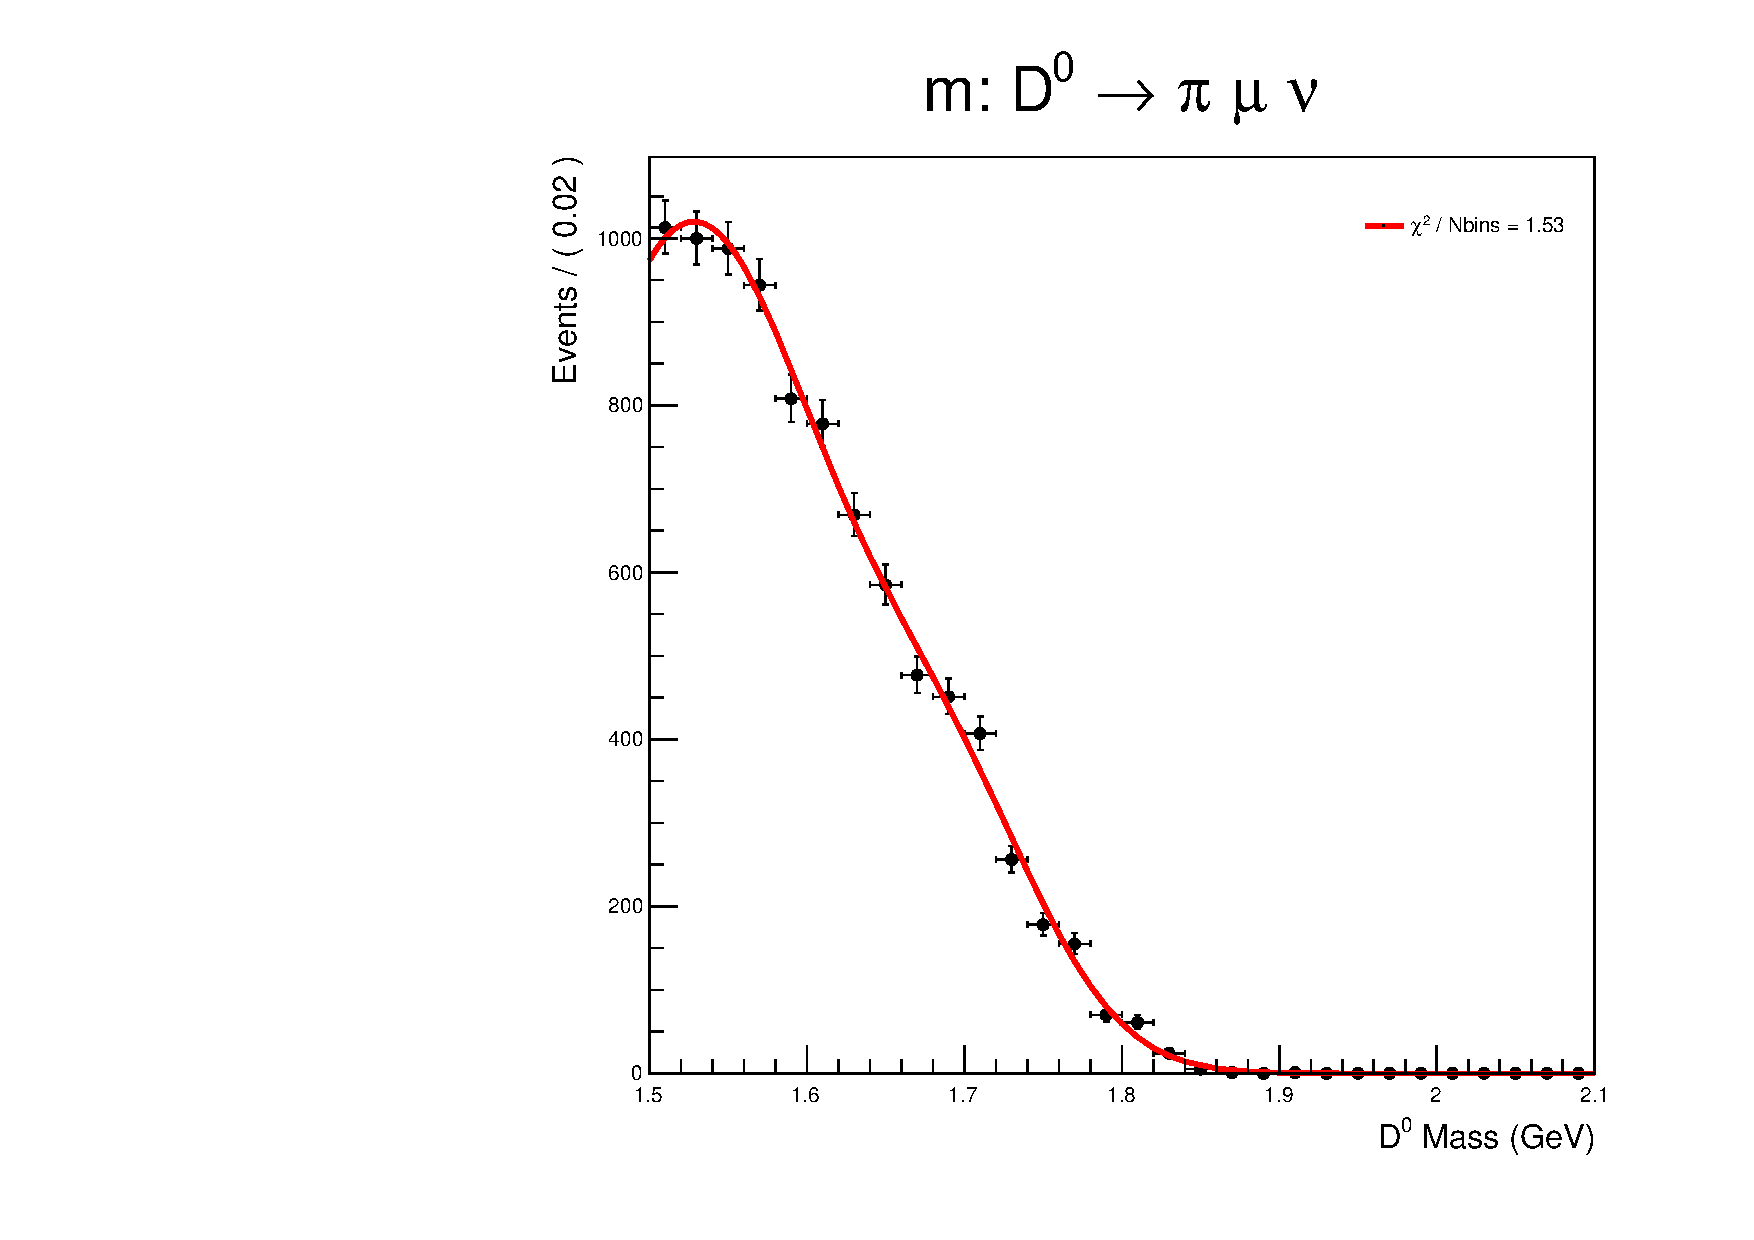
\includegraphics[width=0.45\textwidth]{figures/chapter4/signal_fit/d0pimunu_2022_2023_0_m.pdf}
      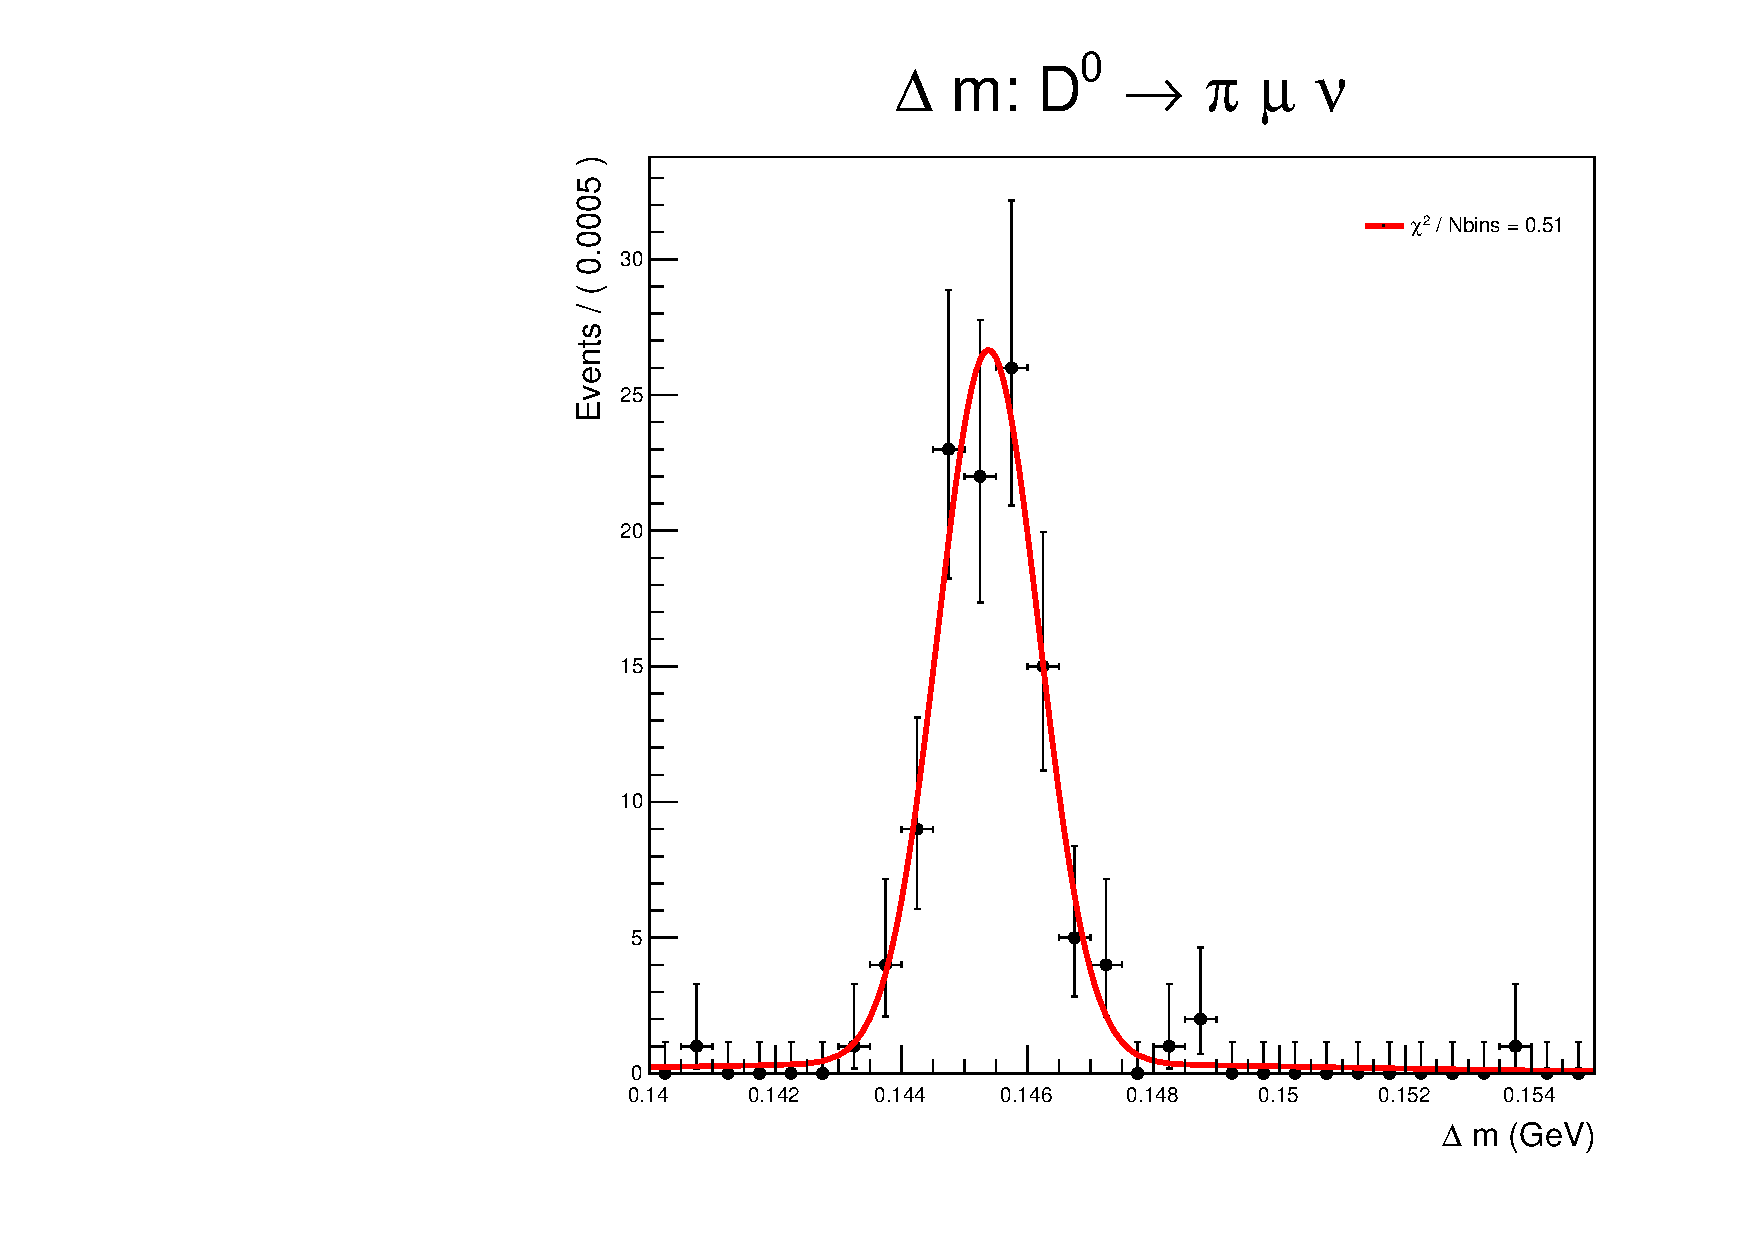
\includegraphics[width=0.45\textwidth]{figures/chapter4/signal_fit/d0pimunu_2022_2023_0_dm.pdf}\\
    \end{center}
    \caption{
      The $D^{*\pm} \to D^0\pi^\pm, D^0 \to \pi^- \mu^+ \nu_\mu$ model fit on MC samples, with $m(D^0)$ displayed left and $\Delta m$ displayed right.
    }
    \label{fig:d0pimunu_uml_fit}
\end{figure}

\begin{figure}[htp]
    \begin{center}
      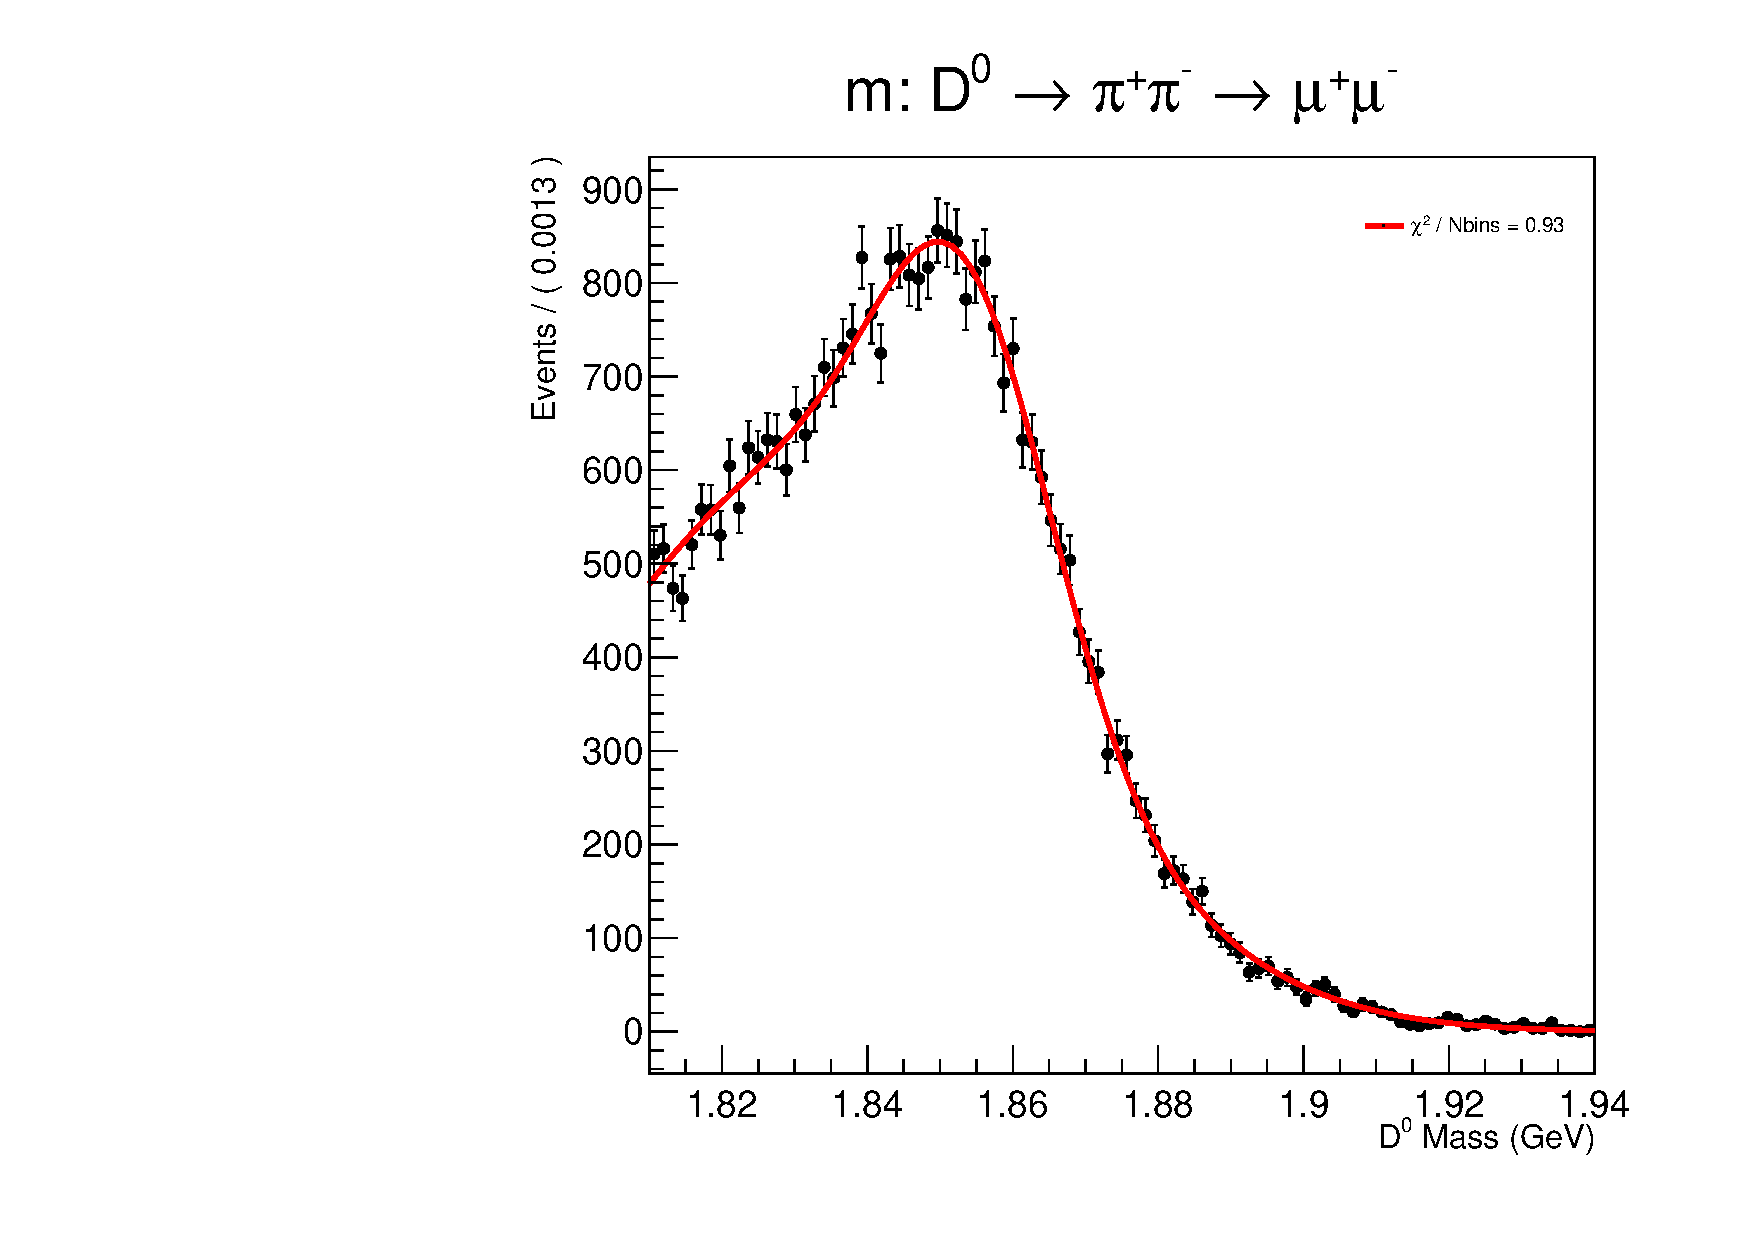
\includegraphics[width=0.45\textwidth]{figures/chapter4/signal_fit/d0pipimm_2022_2023_0_m.pdf}
      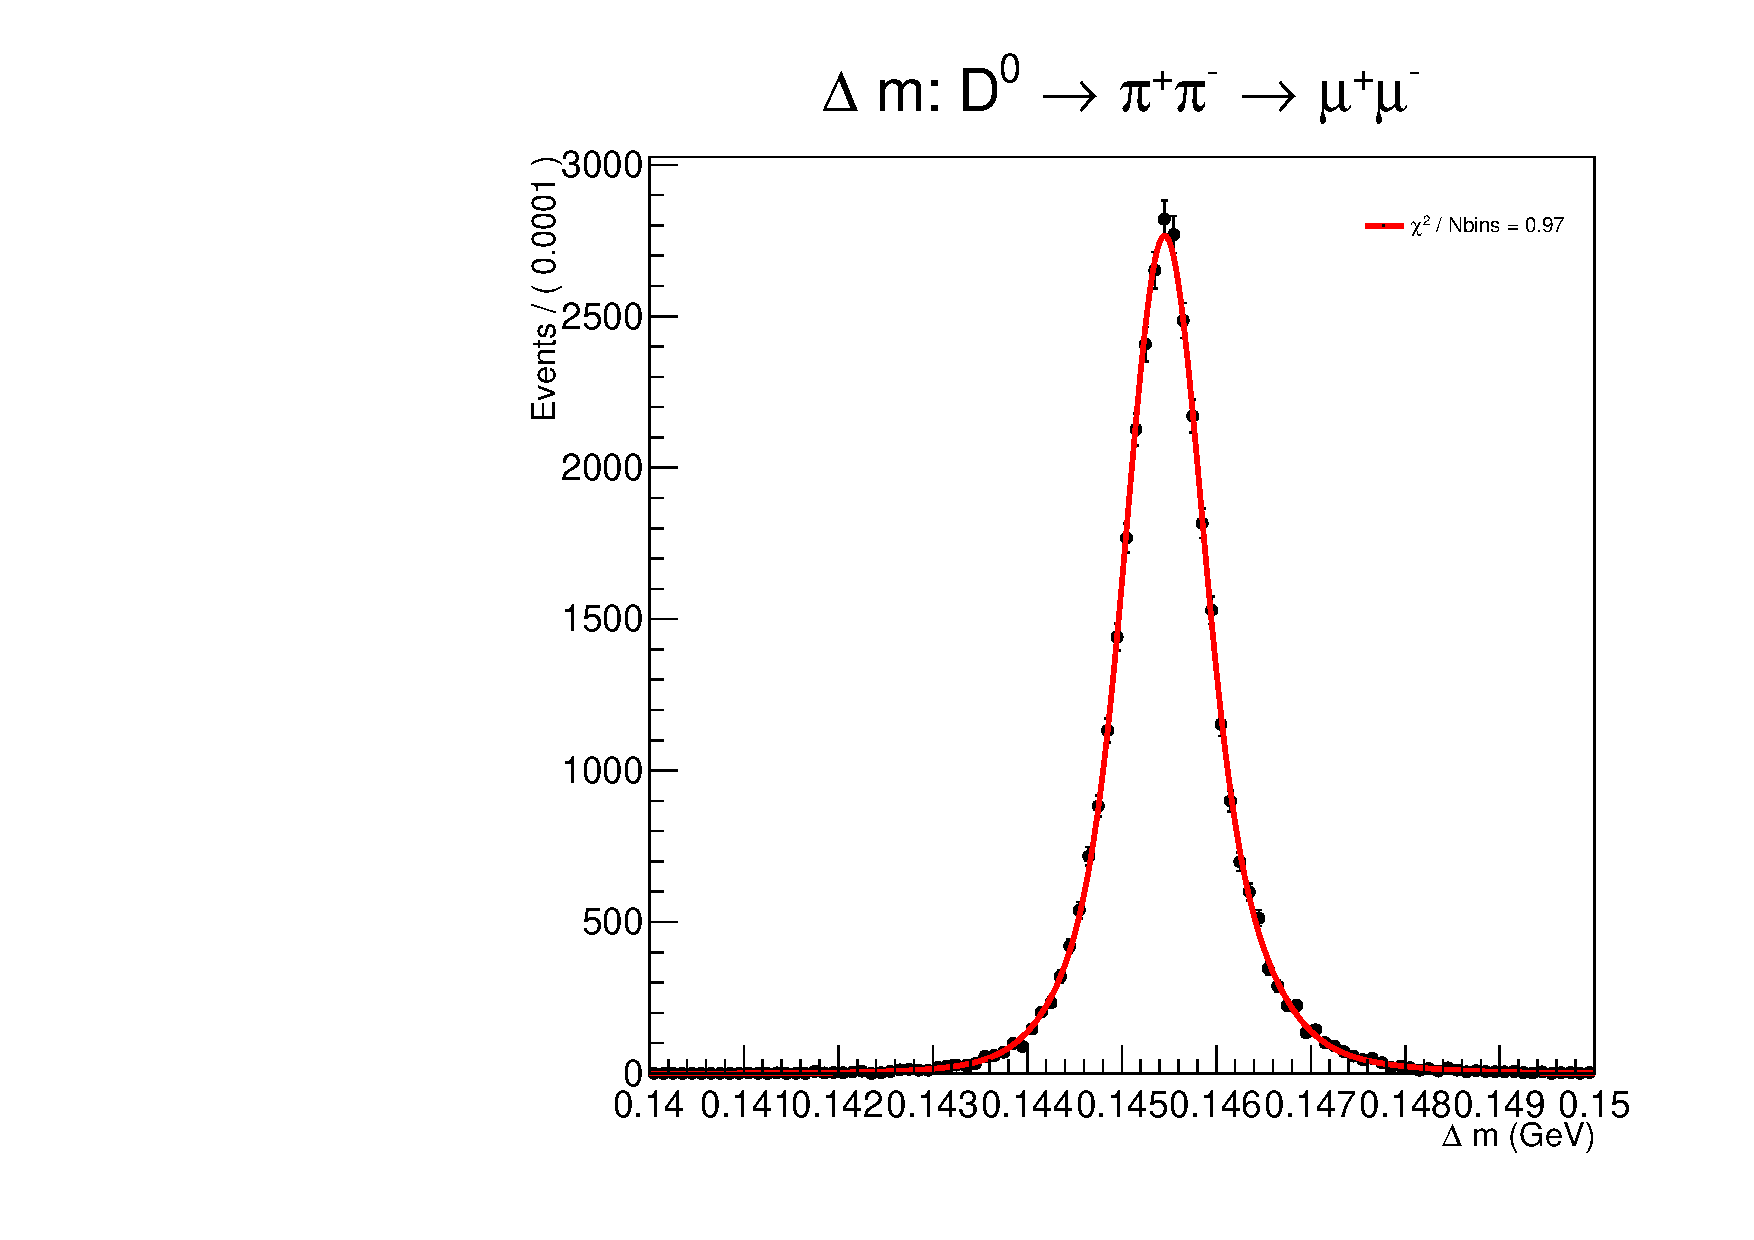
\includegraphics[width=0.45\textwidth]{figures/chapter4/signal_fit/d0pipimm_2022_2023_0_dm.pdf}\\
    \end{center}
    \caption{
      The $D^{*\pm} \to D^0\pi^\pm, D^0 \to \pi^+ \pi^- \to \mu^+ \nu_\mu \mu^- \bar{\nu}_\mu$ model fit on MC samples, with $m(D^0)$ displayed left and $\Delta m$ displayed right.
    }
    \label{fig:d0munumunu_uml_fit}
\end{figure}


The process for determining the combinatorial model is kept the same as for the normalization channel. The only difference is that due to the added complexity of the backgrounds, the $m(D^0)$ pdf function is a combination of a Bernstein polynomial, power law, and exponential function, instead of just an exponential function as was used in the normalization channel \cite{ref:dauncey_2015}. Similar to the normalization channel, the shape and yield is determined using data side-bands, leaving no combinatorial variables left to fit in the main data region. The convergence of the combinatorial fit using partially unblinded data sidebands can be seen in figure \ref{fig:signal_comb_uml_fit}.

\begin{figure}[htp]
    \begin{center}
      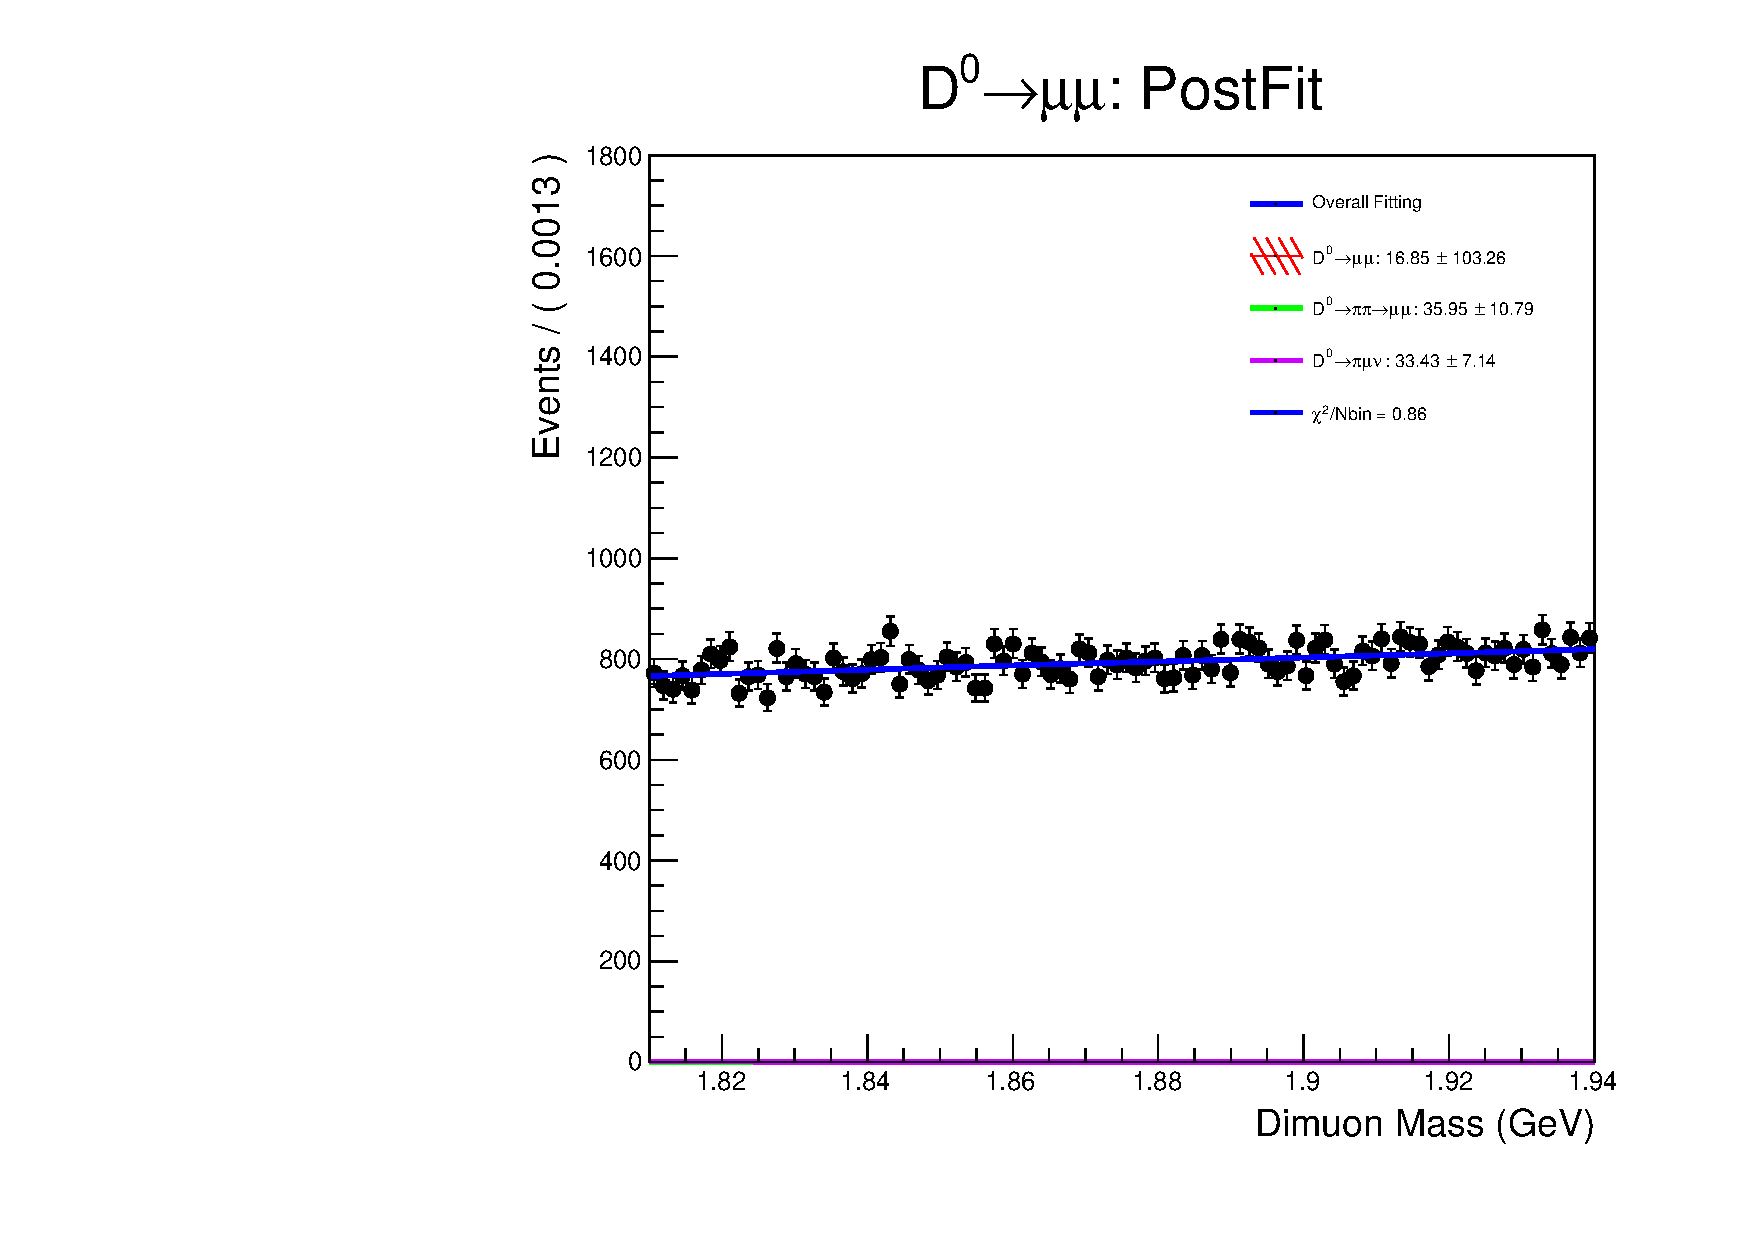
\includegraphics[width=0.45\textwidth]{figures/chapter4/signal_fit/partial_fit_m.pdf}
      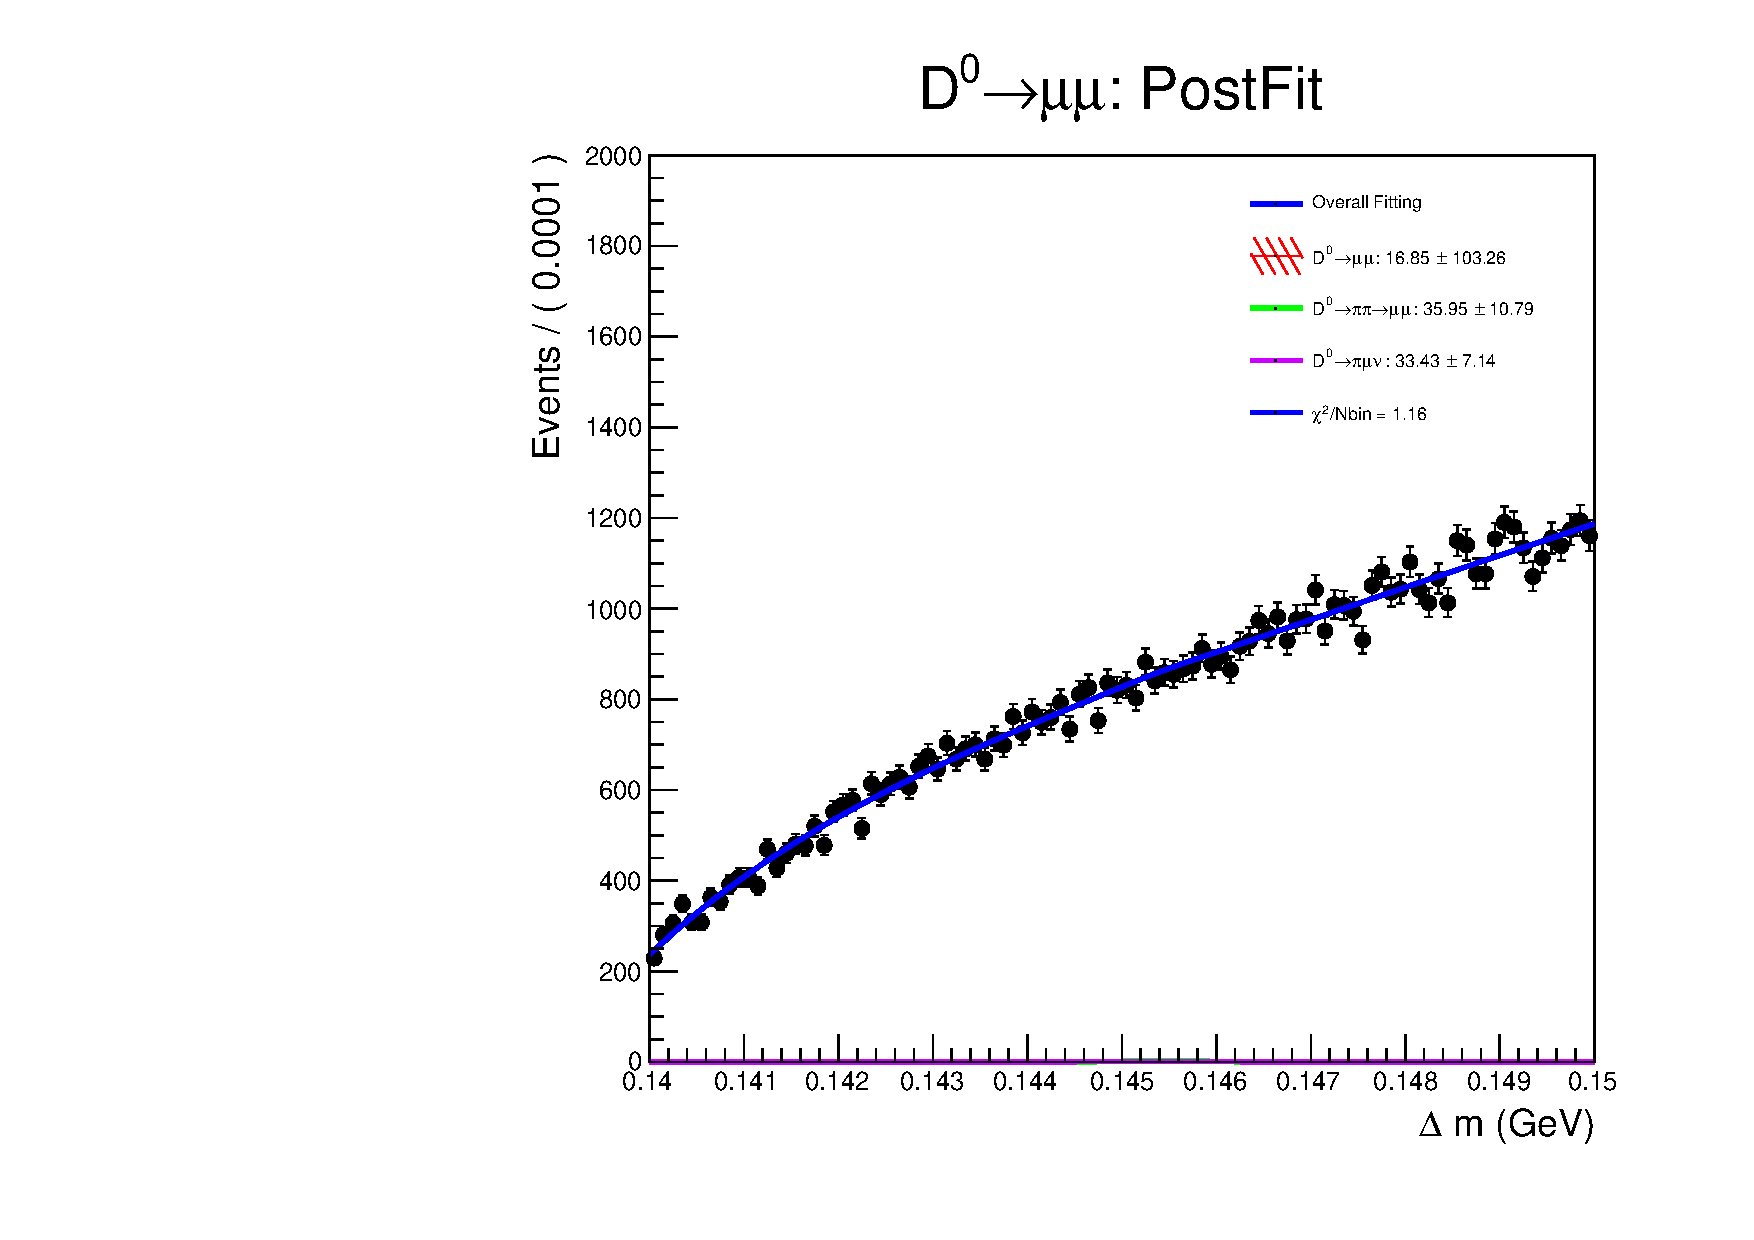
\includegraphics[width=0.45\textwidth]{figures/chapter4/signal_fit/partial_fit_dm.pdf}\\
    \end{center}
    \caption{
      The fit to partial unblinded data before any $\text{MVA}_D$ cut, demonstrating the stability of the combinatorial shape which dominates the overall shape.
    }
    \label{fig:signal_comb_uml_fit}
\end{figure}

\subsubsection{Fit Results}

The final model used for the fit is a sum of signal model and all the background models. One important note is to emphasize that the signal shape and peaking background shape are entirely deriving from MC, the peaking background yeild is determined from equation \ref{eq:peaking_background_yield_calculation}, and combinatorial background shape and yield are determined by the data side-bands. Therefore, the only parameter of this fit is the actual parameter of interest, namely the $N_{D^0 \to \pi^+ \pi^-}$ events. 

The results of this fit are only seen after unblinding the data in as discussed in section \ref{sec:analysis_overview}. The results are presented in section \ref{subsec:final_result}.

\section{Muon Fake Rates}
\label{sec:muon_fake_rate}

A muon fake occurs in this analysis when a pion decay product is measured as muon. This most commonly occurs due to in-flight pion decays, $\pi \to \mu \nu$, but can also occur due to detector misreconstruction. As a result, the more common $D^0 \to \pi^+ \pi^-$ process can mimic genuine $D^0 \to \mu^+ \mu^-$ events when the pions decay in flight, producing muons that are misidentified as signal and causing a significant challenge to this analysis. Therefore, a clear and precise understanding of the muon fake rate must be achieved to be used throughout the rest of the analysis. The below method was first developed to search for the $B^0 \to \mu^+ \mu^-$ decay \cite{ref:2023b0mumu}. Below we summarize the most relevant aspects of the procedure and results for the \texttt{Loose} muon identification system, the \texttt{highPurity} inner track quality requirements, tracker muon, and global muon requirements. These requirements reflect the selection critierion for the rest of the analysis described in section \ref{subsec:preselection} and section \ref{subsec:baseline_selection}.

\subsection{Data Samples and Selections}

To get a reliable prediction for muon fake rates we need to be able to simulate pion decays in flight. We also needed to be able to simulate reconstructing the pion as a muon candidate through a muon identification scheme. While pion decays into muons can be simulated with adequate precision in MC, the reconstruction and muon identification parts are harder to simulate correctly. Therefore, we need to be able to measure the fake rates in data, then use those results to correct MC predictions. To increase the sensitivity of the fake rate measurement, we use control samples that clearly identify hadrons in data and MC. Additionally, to avoid a dependence on the trigger, we pick samples with triggers that only fire on  electrons. Using this, we remove trigger dependence on muons, removing a trigger  bias toward muons from the sample. Thus, the data samples used is in this anaylsis are \texttt{EGamma (2022)}, \texttt{EGamma0 (2023)}, \texttt{Egamma1 (2023)}, and \texttt{ParkingDoubleElectronLowMass}. The \texttt{EGamma} datasets require events to pass single-electron triggers, while \texttt{ParkingDoubleElectronLowMass} relies on low-mass dielectron triggers with reduced prescales, enabling efficient selection of low-momentum hadronic decays.

For MC studies of muon fake rates, several background samples are used to provide a realistic modeling of processes that can produce hadrons misidentified as muons. Drell-Yan samples with dileptons and two associated jets are included, both in the low-mass (10-50 GeV) and high-mass (above 50 GeV) regimes, generated using the \texttt{amcatnloFXFX} and \texttt{madgraphMLM} frameworks interfaced with \texttt{pythia8}. A dedicated sample of Drell-Yan to dielectrons is also included to help disentangle muon-specific effects. Additionally, \texttt{$W\to l \nu$} events with jets and \texttt{t$\bar{\text{t}}$} events in the lepton+jets final state are included to capture fake muons arising in high-activity environments with real leptons and multiple jets. All samples are produced at $\sqrt{s} = 13.6$ TeV and use the \texttt{TuneCP5} parton shower configuration.

To study muon fakes originating from pions we use $K_S^0 \to \pi^+ \pi^-$ control sample. The selection requirements are:
\begin{itemize}
\item $p_{T}^{\pi_1}>1$ GeV
\item $p_{T}^{\pi_2}>4$ GeV
\item pion track is highPurity
\item $m_{K_S^0}\in[0.45,0.55]$
\item $\frac{L_{xy}}{\sigma_L}>3$
\item Vertex probability greater than 0.001
\item vertex displacement in XY plane wrt Beam Spot less than 8
\item cosine of pointing angle in XY wrt BS greater than 0.999
\item impact parameter significance of the candidate trajectory in 3D wrt PV less than 3
\item 2D impact parameter significance for Track 1 and 2 wrt Beam Spot greater than 5
\item kinematic vertex fit $\chi^{2}/dof$ of the two track less than 3
\item Fire the HLT Electron30 trigger
\end{itemize}


\subsection{Measurement Procedure}

To measure the fake rate we perform an extended binned maximum likelihood fit to
$\pi^{+}\pi^{-}$ and $\mu^{\pm}\pi^{\pm}$ invariant mass distribution to extract
the event yield of $K_S^0 \to \pi^+ \pi^-$ and $K_S^0 \to \mu^\pm \pi^\mp$ events. The model used to describe the signal and combinatorial background component are a Crystall Ball added to a  Gaussian centered at the same mean and a 2nd order Bernstein polynomial function, respectively. The signal shape in the $K_S^0 \to \mu^\pm \pi^\mp$ distribution is fixed from the $K_S^0 \to \pi^+ \pi^-$  distribution to avoid the different signal shape due to the low statistics. One of the fit projection is shown in the figure~\ref{fig:fit_example_pion}

\begin{figure}[!h]
  \begin{center}
    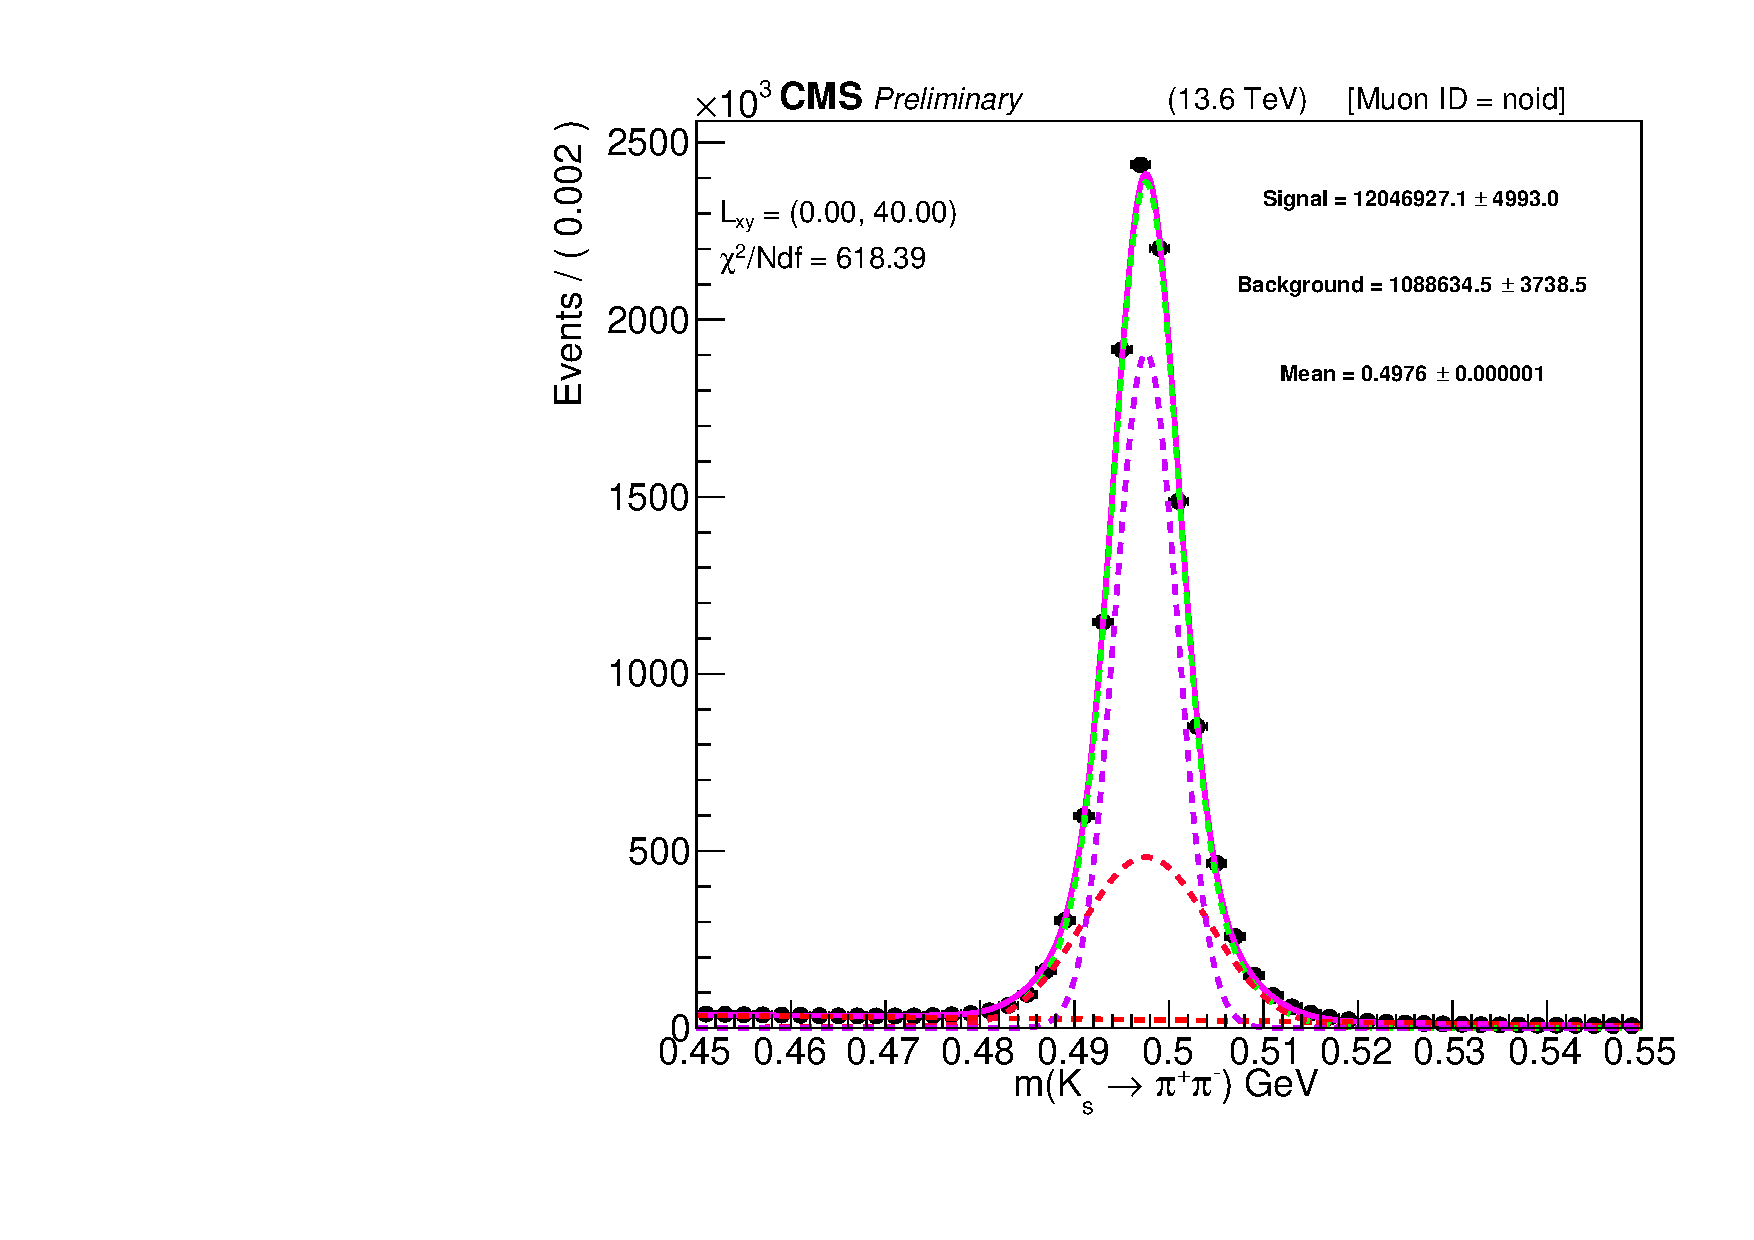
\includegraphics[width=0.45\textwidth]{figures/chapter4/fakerate/Combined_data_combined_522_2022_ks_trigger_lxy_hv0_Mass_allbin_bla.pdf}
    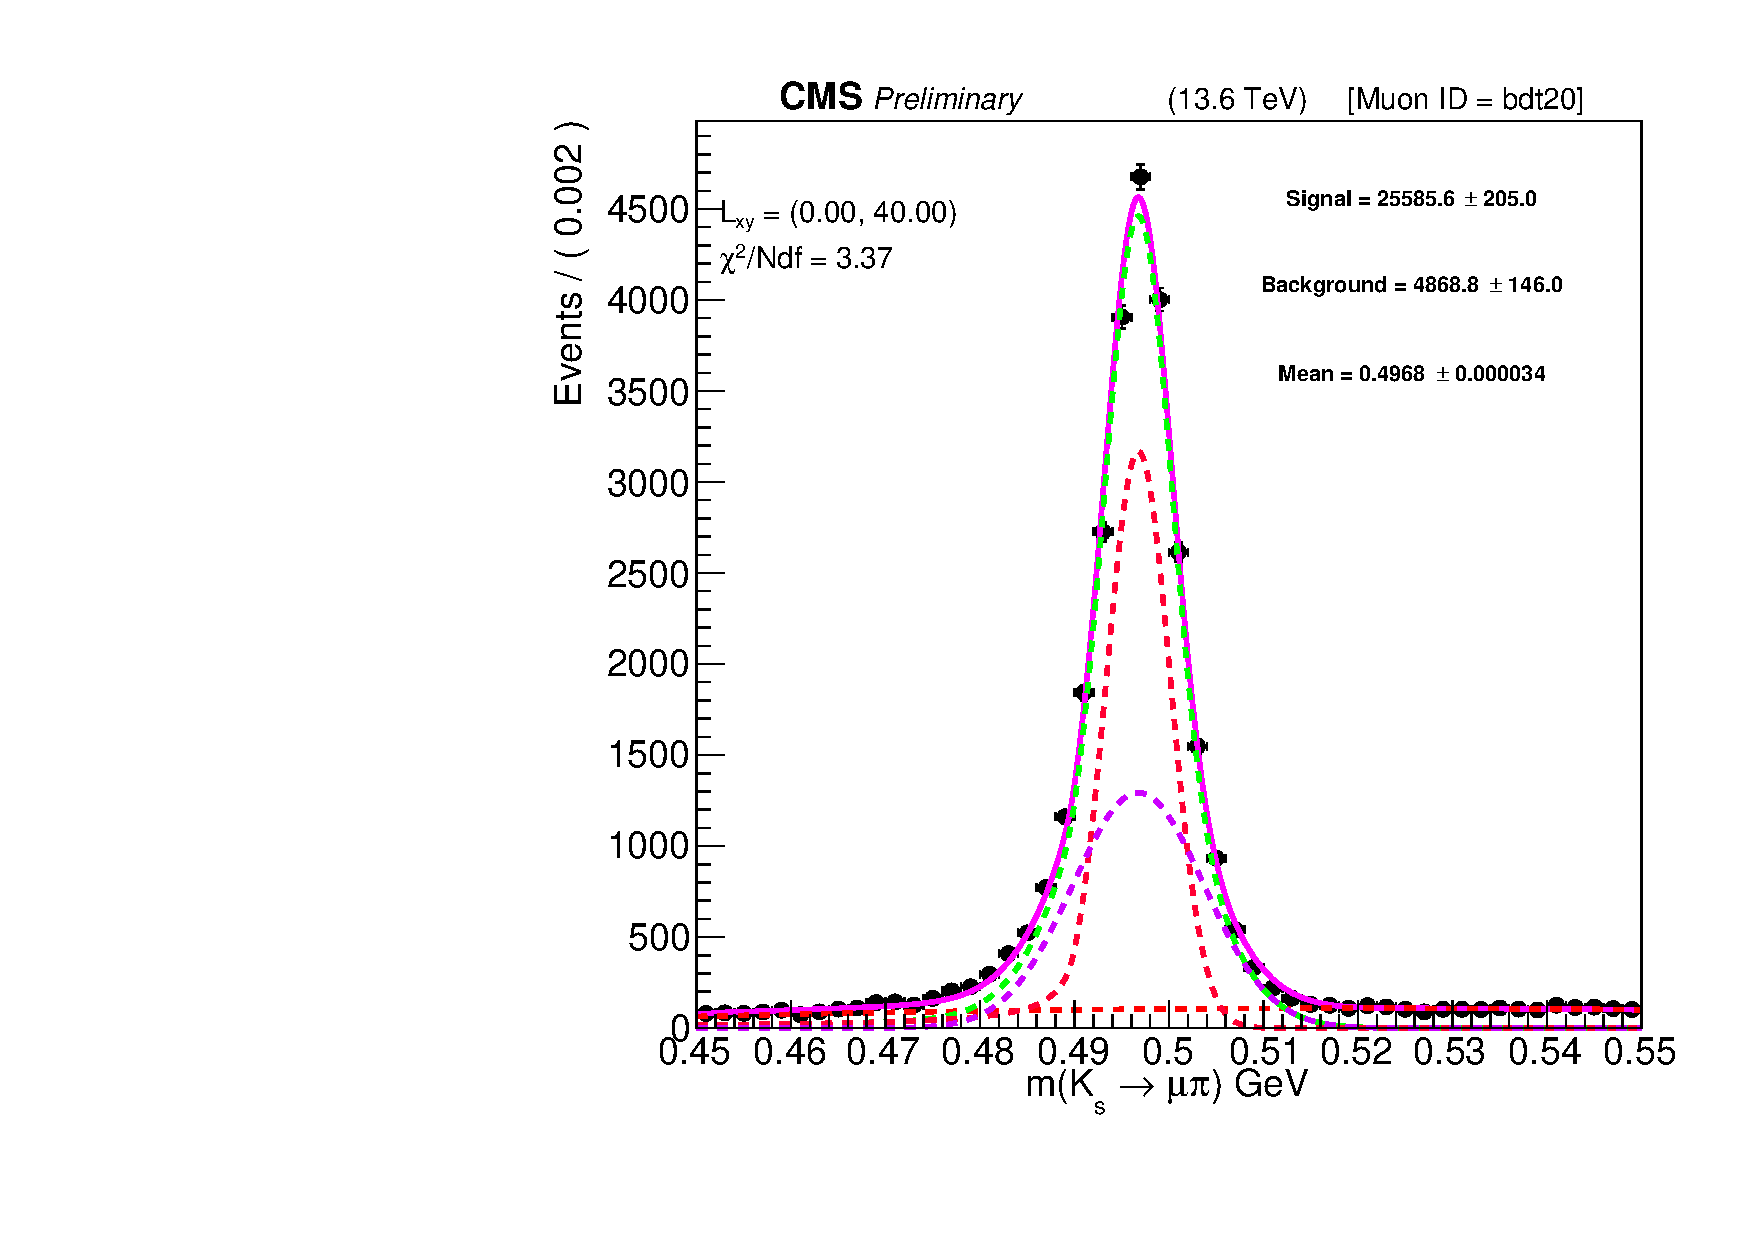
\includegraphics[width=0.45\textwidth]{figures/chapter4/fakerate/Combined_data_combined_522_2022_ks_trigger_lxy_hv0_Mass_muid_20_allbin_bla.pdf}\\
  \end{center}
  \caption{Invariant mass projection from $K_S^0 \to \pi^+ \pi^-$ decays in the $\mu$
    $p_{T}$ range 4-40.0 GeV using 2022 data before (left) and after(right) soft muon MVA ID cut.
    The green dashed line is for the signal distribution, the red
    dotted line is for combinatorial background, and the result of the
    fit projection is the solid pink line. The data are shown with
    solid black circles.}
  \label{fig:fit_example_pion}
\end{figure}

The fake rate is estimated in bins of muon $p_{T}$. For each $K_S^0 \to \pi^+ \pi^-$ candidate we check $p_{T}$ and acceptance for both pions and add the $K_S^0$ candidate to the appropriate $p_{T}$ bin (\ref{fig:fakerates}).

\begin{figure}[!h]
  \begin{center}
    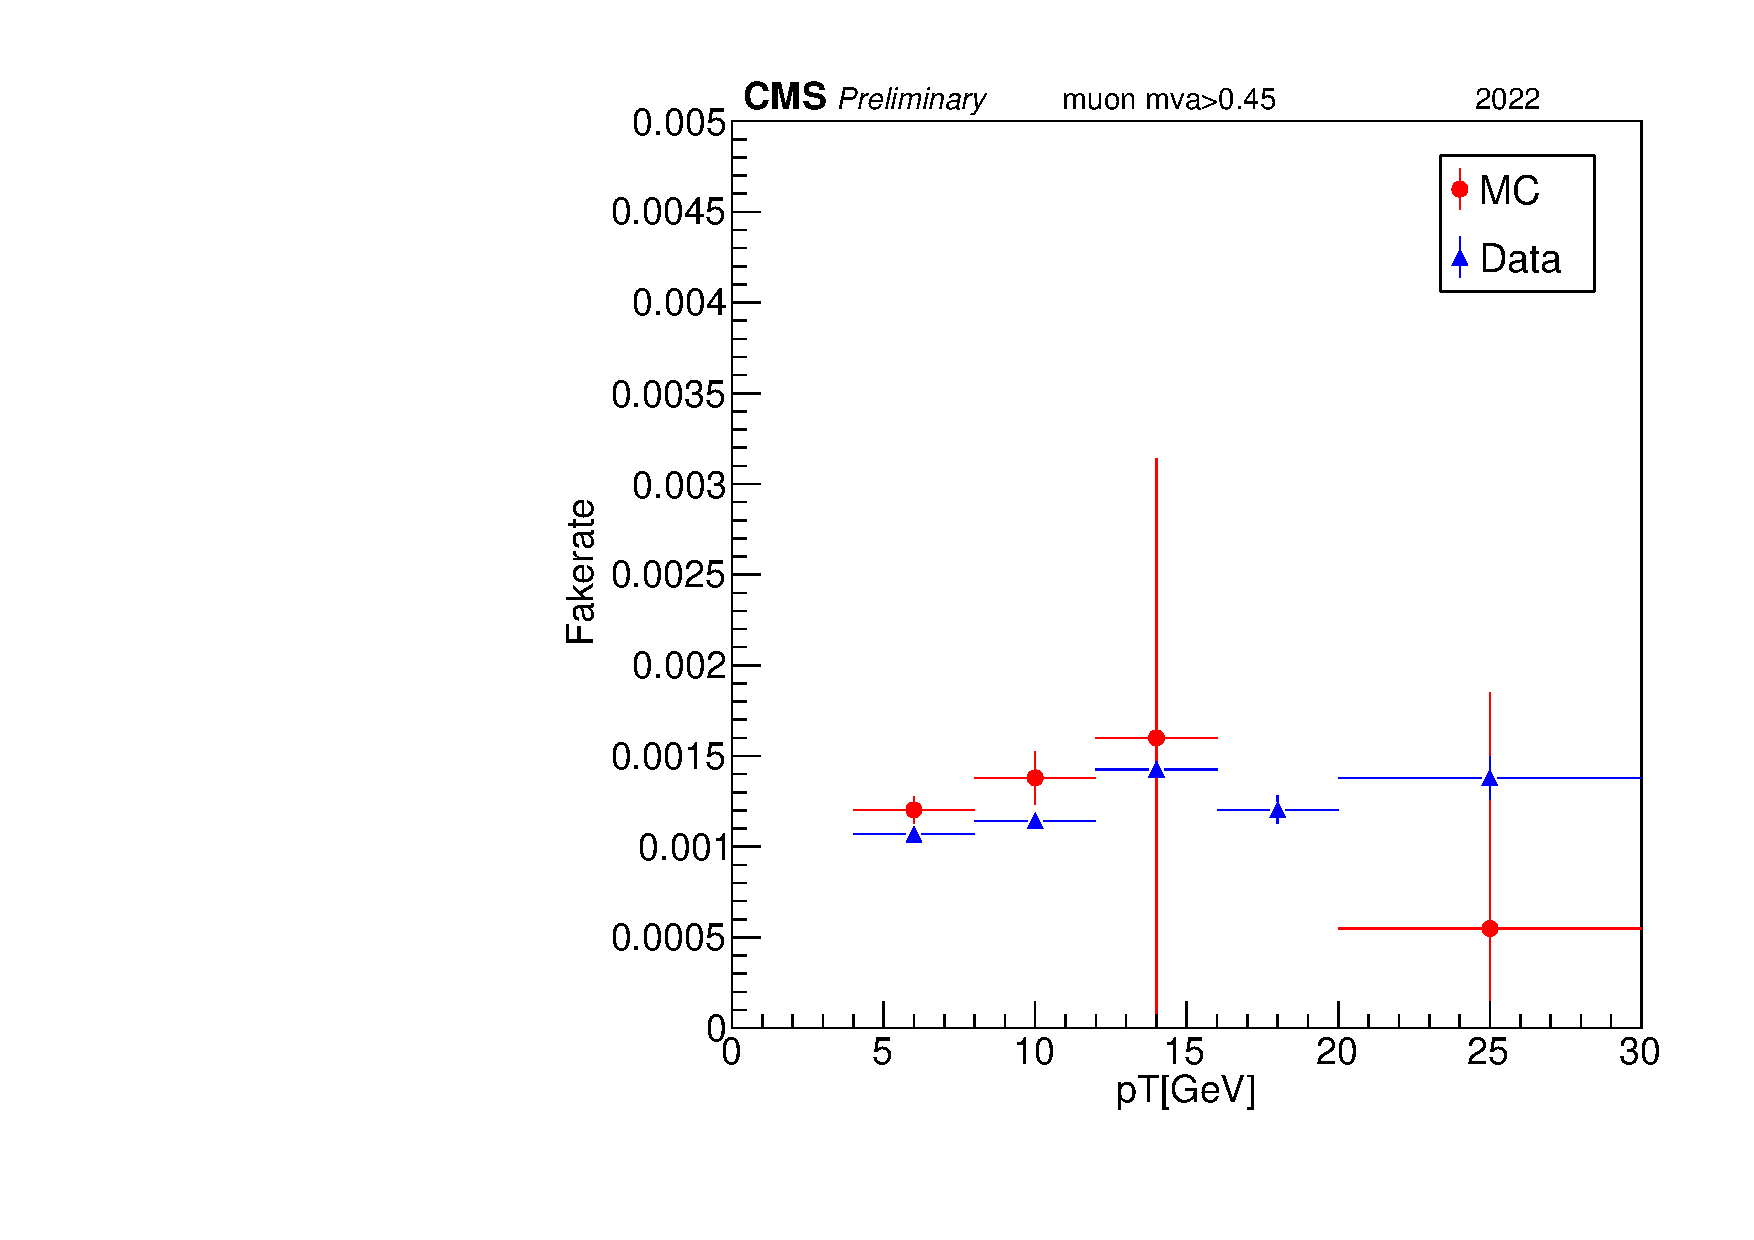
\includegraphics[width=0.45\textwidth]{figures/chapter4/fakerate/Run2022_pion-fakes.pdf}
    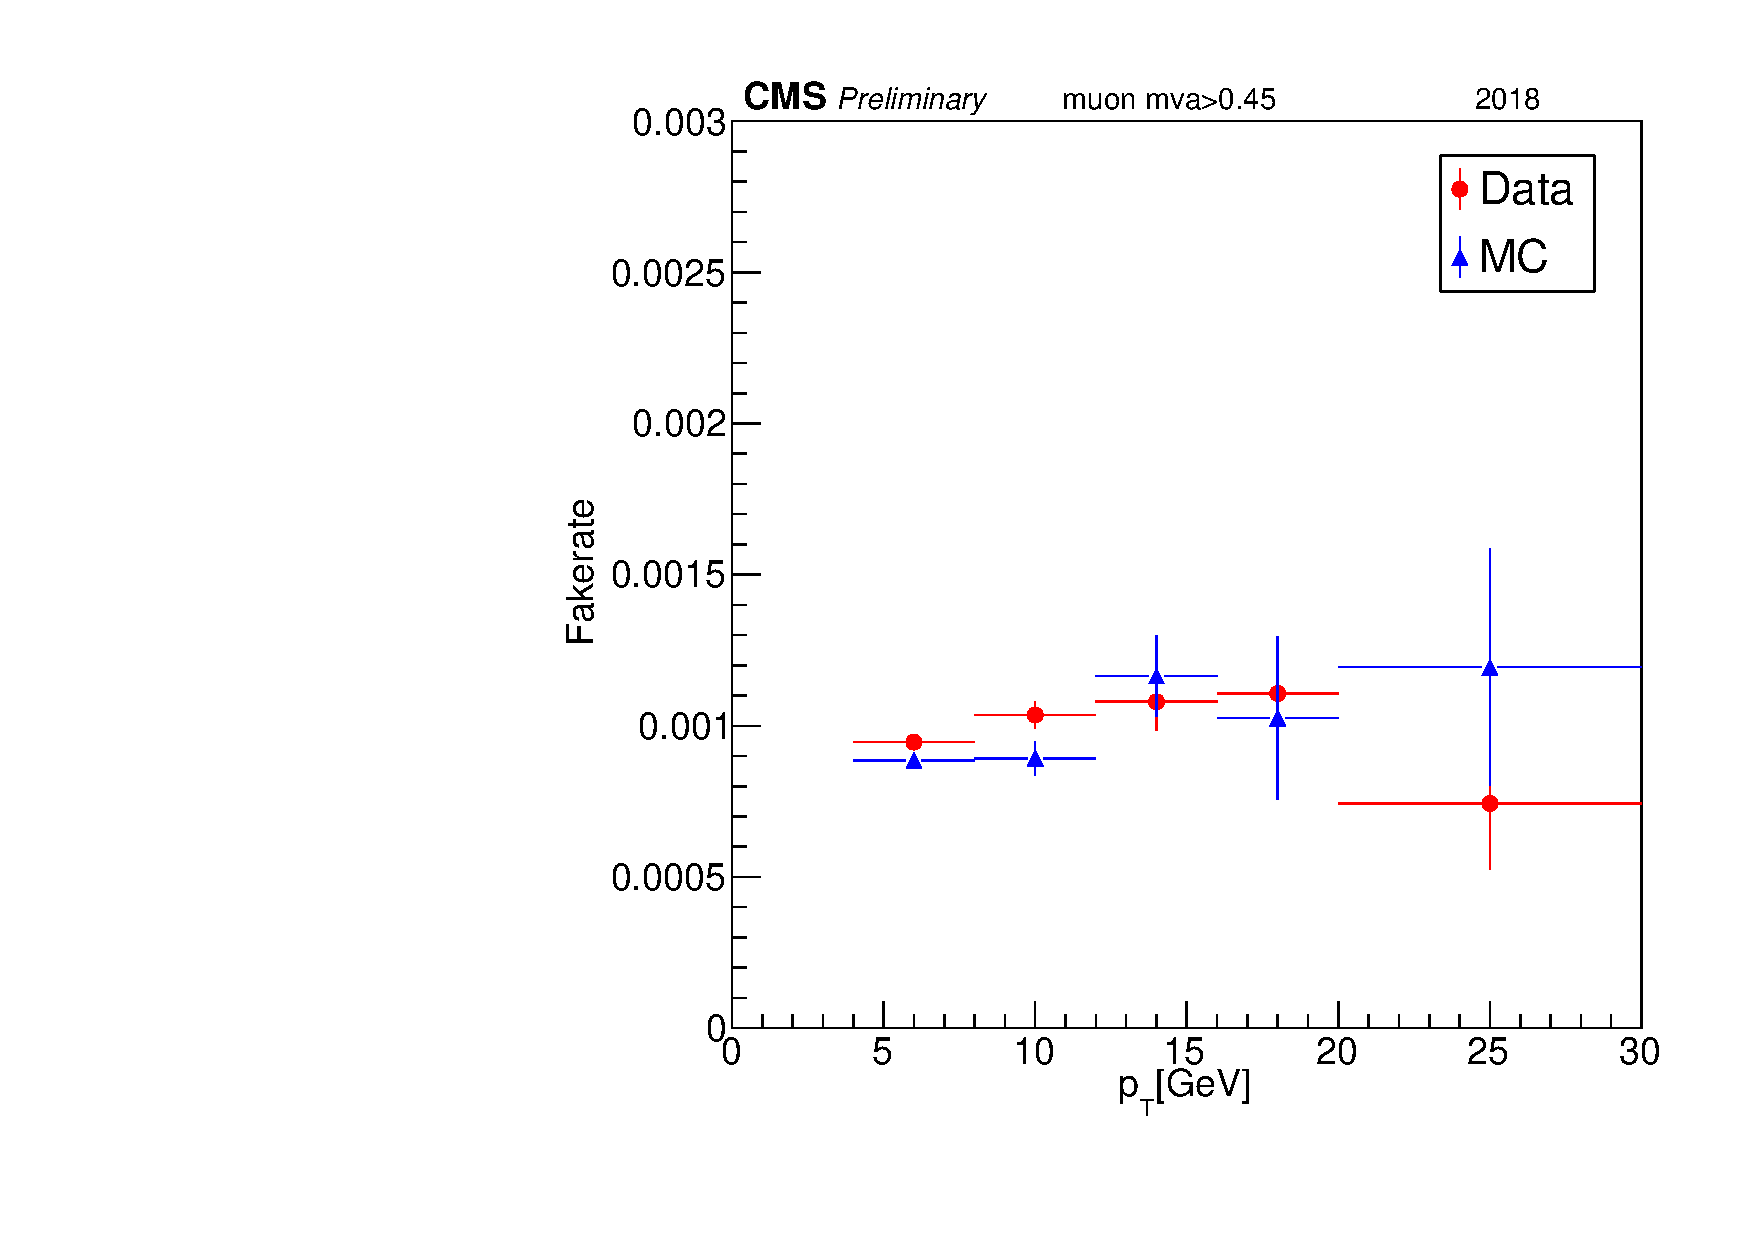
\includegraphics[width=0.45\textwidth]{figures/chapter4/fakerate/Run2023_pion-fakes.pdf}
    \caption{Pion muon fake rates for Run2022 (top) and
      Run2023 (bottom) as a function muon $p_{T}$.}
    \label{fig:fakerates}
  \end{center}
\end{figure}


The fake rate estimated from $K_S^0$ decays also has a dependence on the $K_S^0$ flight length (Figure \ref{fig:pion_fake_rate_fs_flight_length}). There are two different trends. The first is the fake rate increase with the flight length, which is most pronounced for the Loose muon selection. The second one shows a dramatic decrease in the fake rate for muon candidates passing the Soft Muon MVA selection when they originate outside of the pixel detector (fligt length greater than 8 cm).

\begin{figure}[!h]
  \begin{center}
    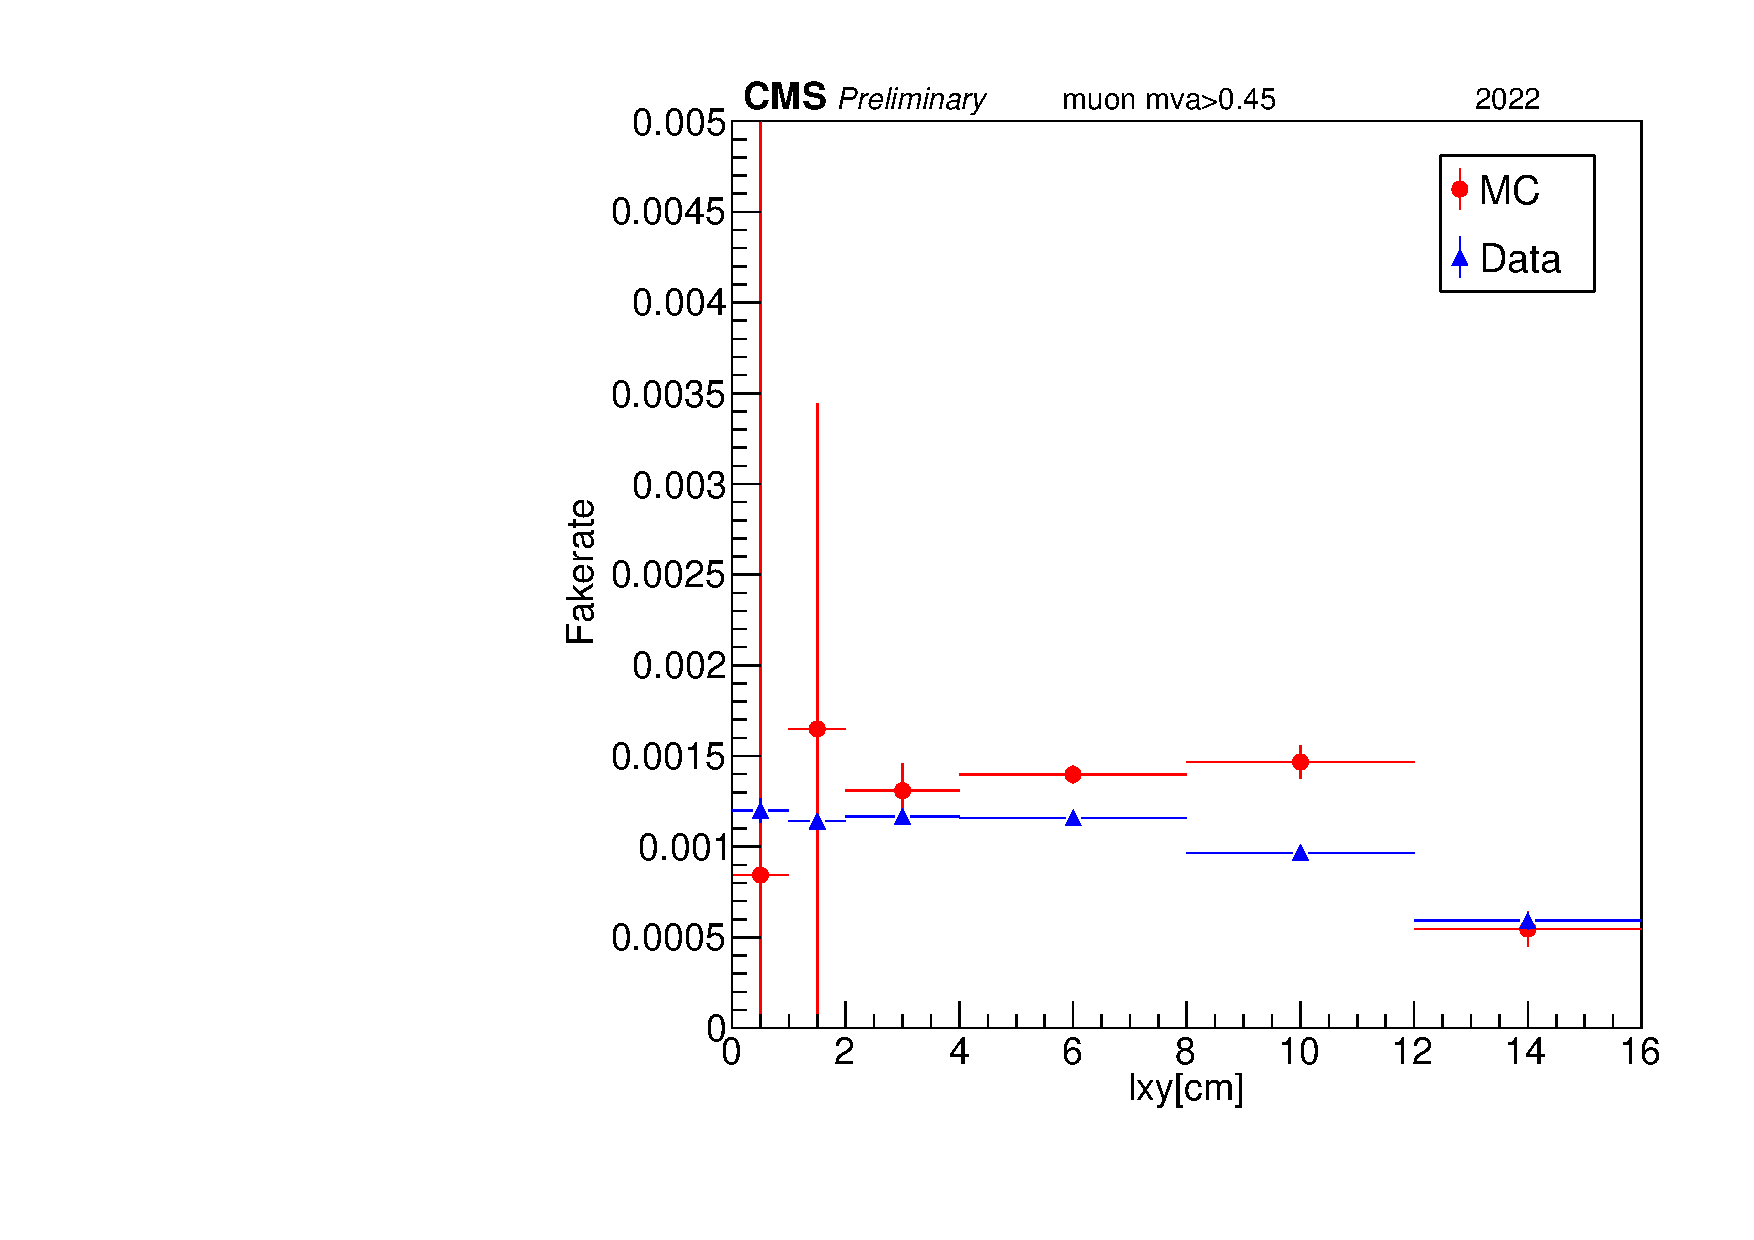
\includegraphics[width=0.45\textwidth]{figures/chapter4/fakerate/playV0-ks_kin_lxy_muidbdt45_MC_v_Data_overlay.pdf}
  \end{center}
  \caption{Fake rate dependence on flight length (lxy) measured in cm for data and MC}
  \label{fig:pion_fake_rate_fs_flight_length}
\end{figure}

Both effects are related to the number of pixel and silicon stip hits for the inner track, which is known to be smaller for fake muons. In the case of the Loose selection this information is not used directly for the muon identification, while for the Soft Muon MVA it is one of the most powerful discriminators. The fact that the fake rate has a non-trivial dependence on the flight length means that we have to match the flight length of the fakes used in the physics analysis to the one available in the control sample. Otherwise, this dependence can lead to a biased measurement of the fake rate since most $K_S^0$ have much larger flight length than the D mesons used in this analysis. Therefore, we restrict the transverse decay length to 8 cm to match the $D$ mesons studied in the analysis. In this region, the fakerate seems to relatively flat and there is enough data to make precise estimates of the fake rate in this region. 

Systematic error for the fake rates measurements in MC samples are derived from taking the weighted differences between the various MC samples used, namely W+Jets, Drell-Yan, and TT bar. Furthermore, systematic error for the fake rate measurements in data is mainly derived  from the differences between EGamma and Parking Electron datasets. Agreement between these datasets can be seen in the plots (\ref{fig:pion_fake_rate_systematics}). To account for the variation in terms of the $l_{xy}$ value, an additional $2\%$ of systematic uncertainty is assigned, motivated by the scale factor variation in terms of $p_T$ and $l_{xy}$ between data collected in 2022 and data collected in 2023. 

The final fake rate results are summarized in table \ref{tab:muon_fake_rate}.

\begin{figure}[!h]
  \begin{center}
    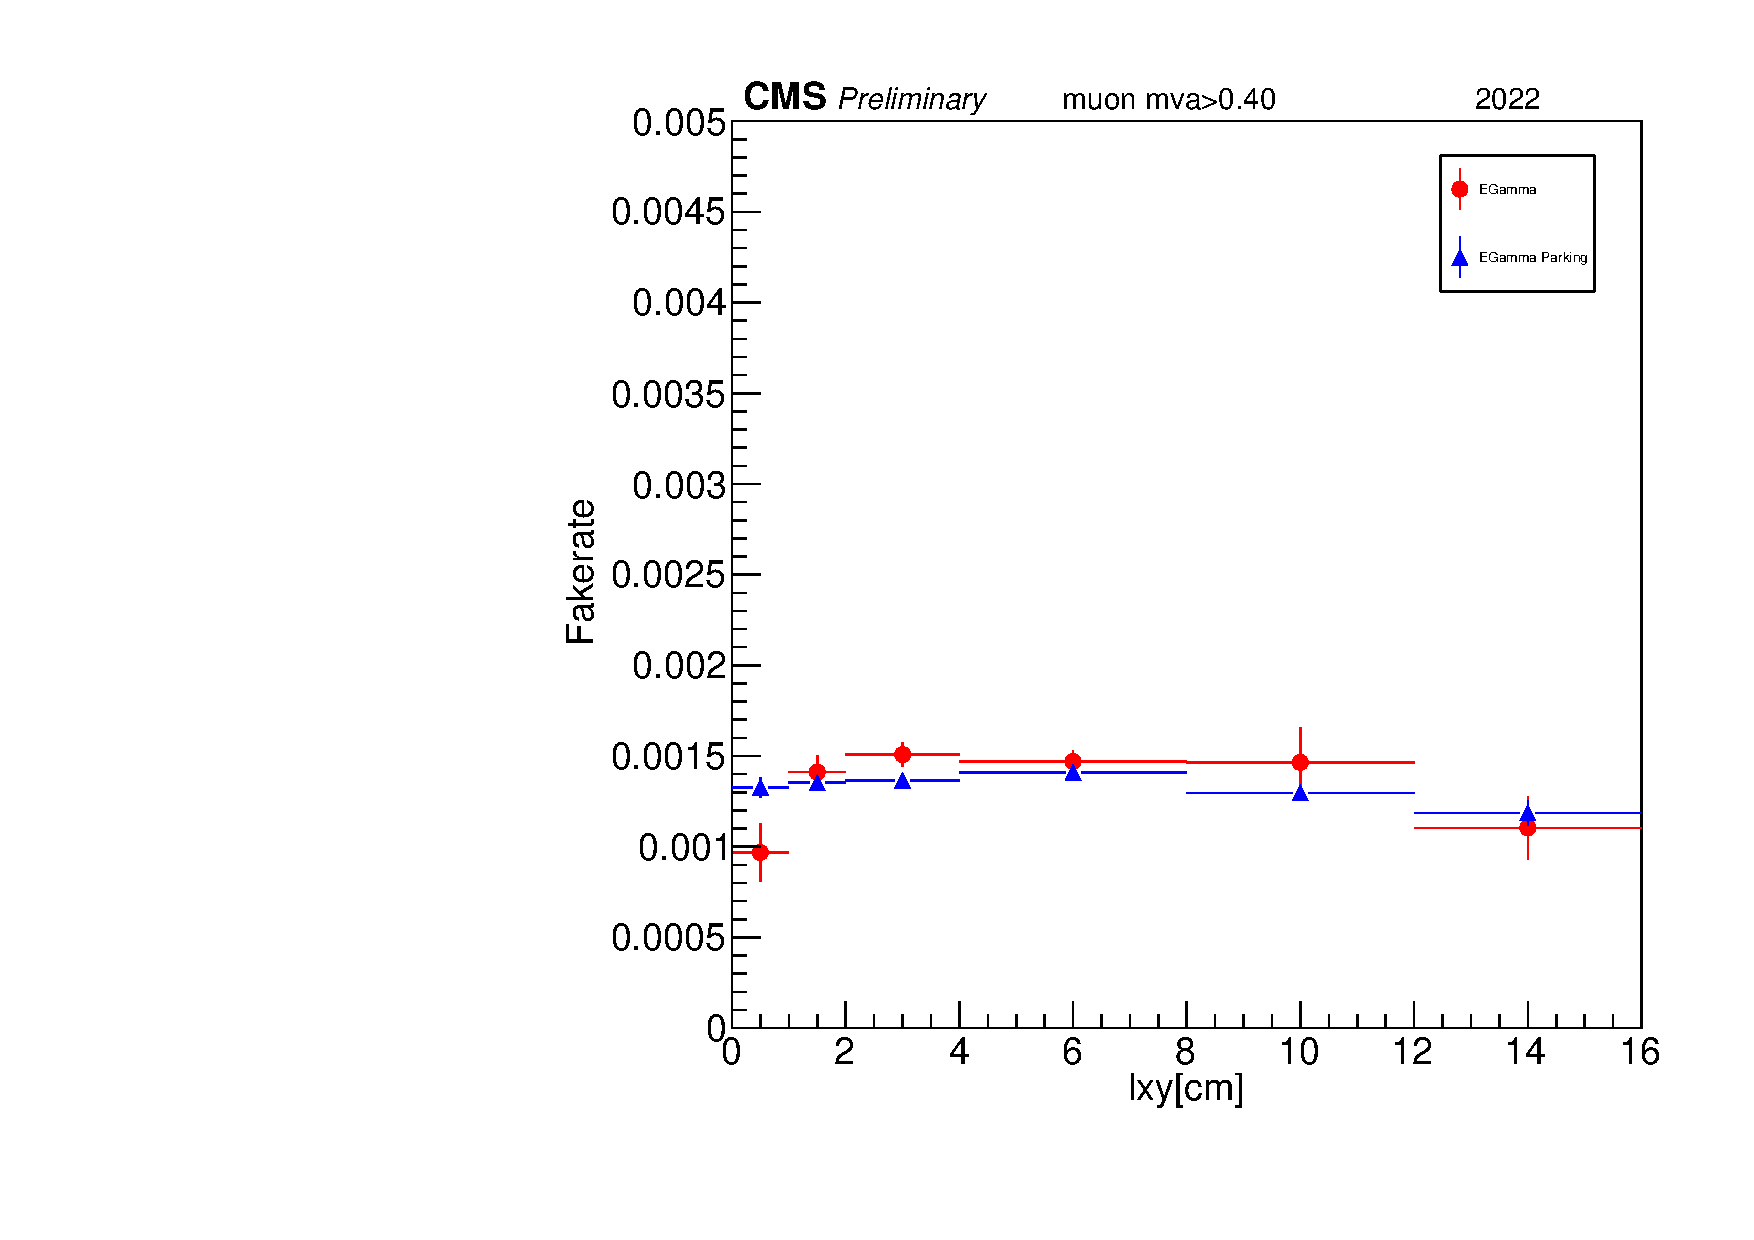
\includegraphics[width=0.45\textwidth]{figures/chapter4/fakerate/playV0-ks_kin_lxy_muidbdt40_EGamma_v_Parking_overlay.pdf}
    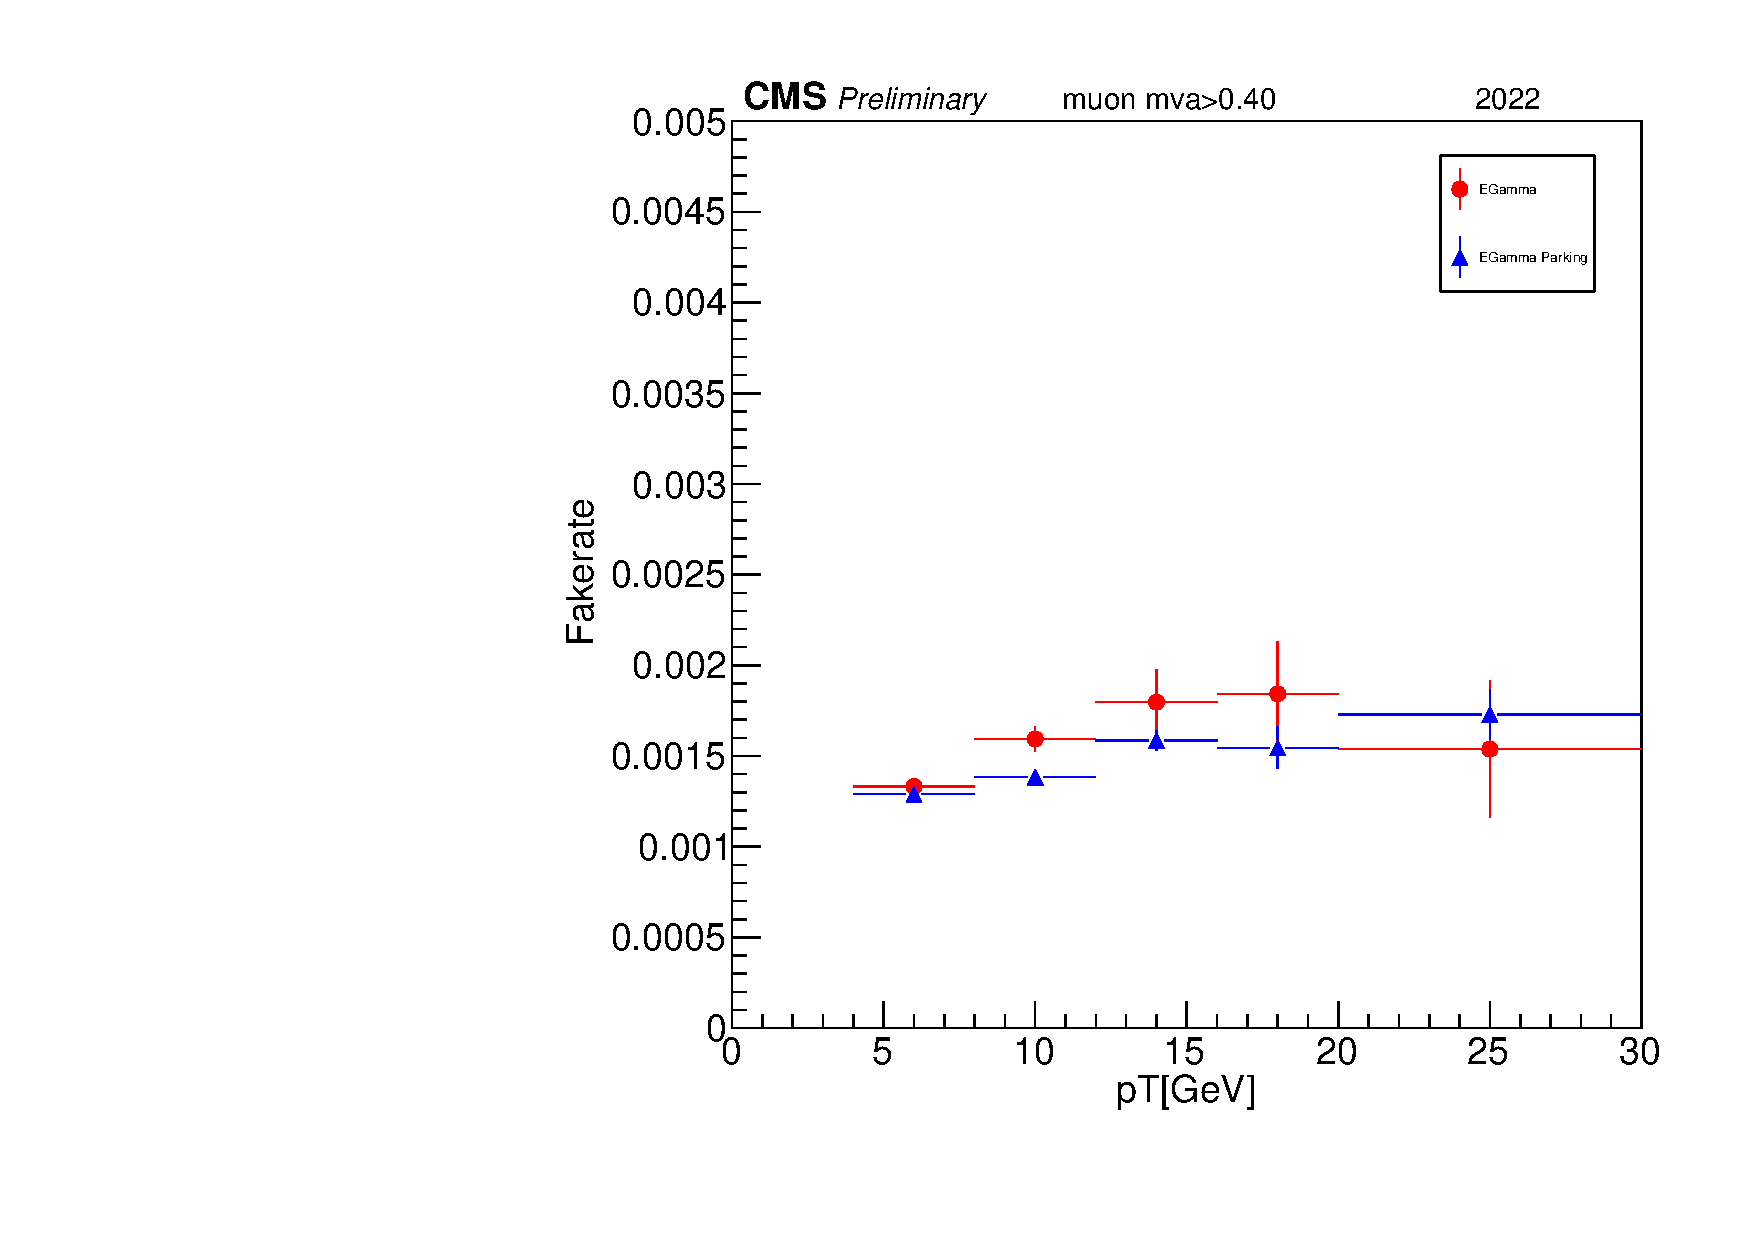
\includegraphics[width=0.45\textwidth]{figures/chapter4/fakerate/playV0-ks_kin_pT_muidbdt40_EGamma_v_Parking_overlay.pdf} \\
    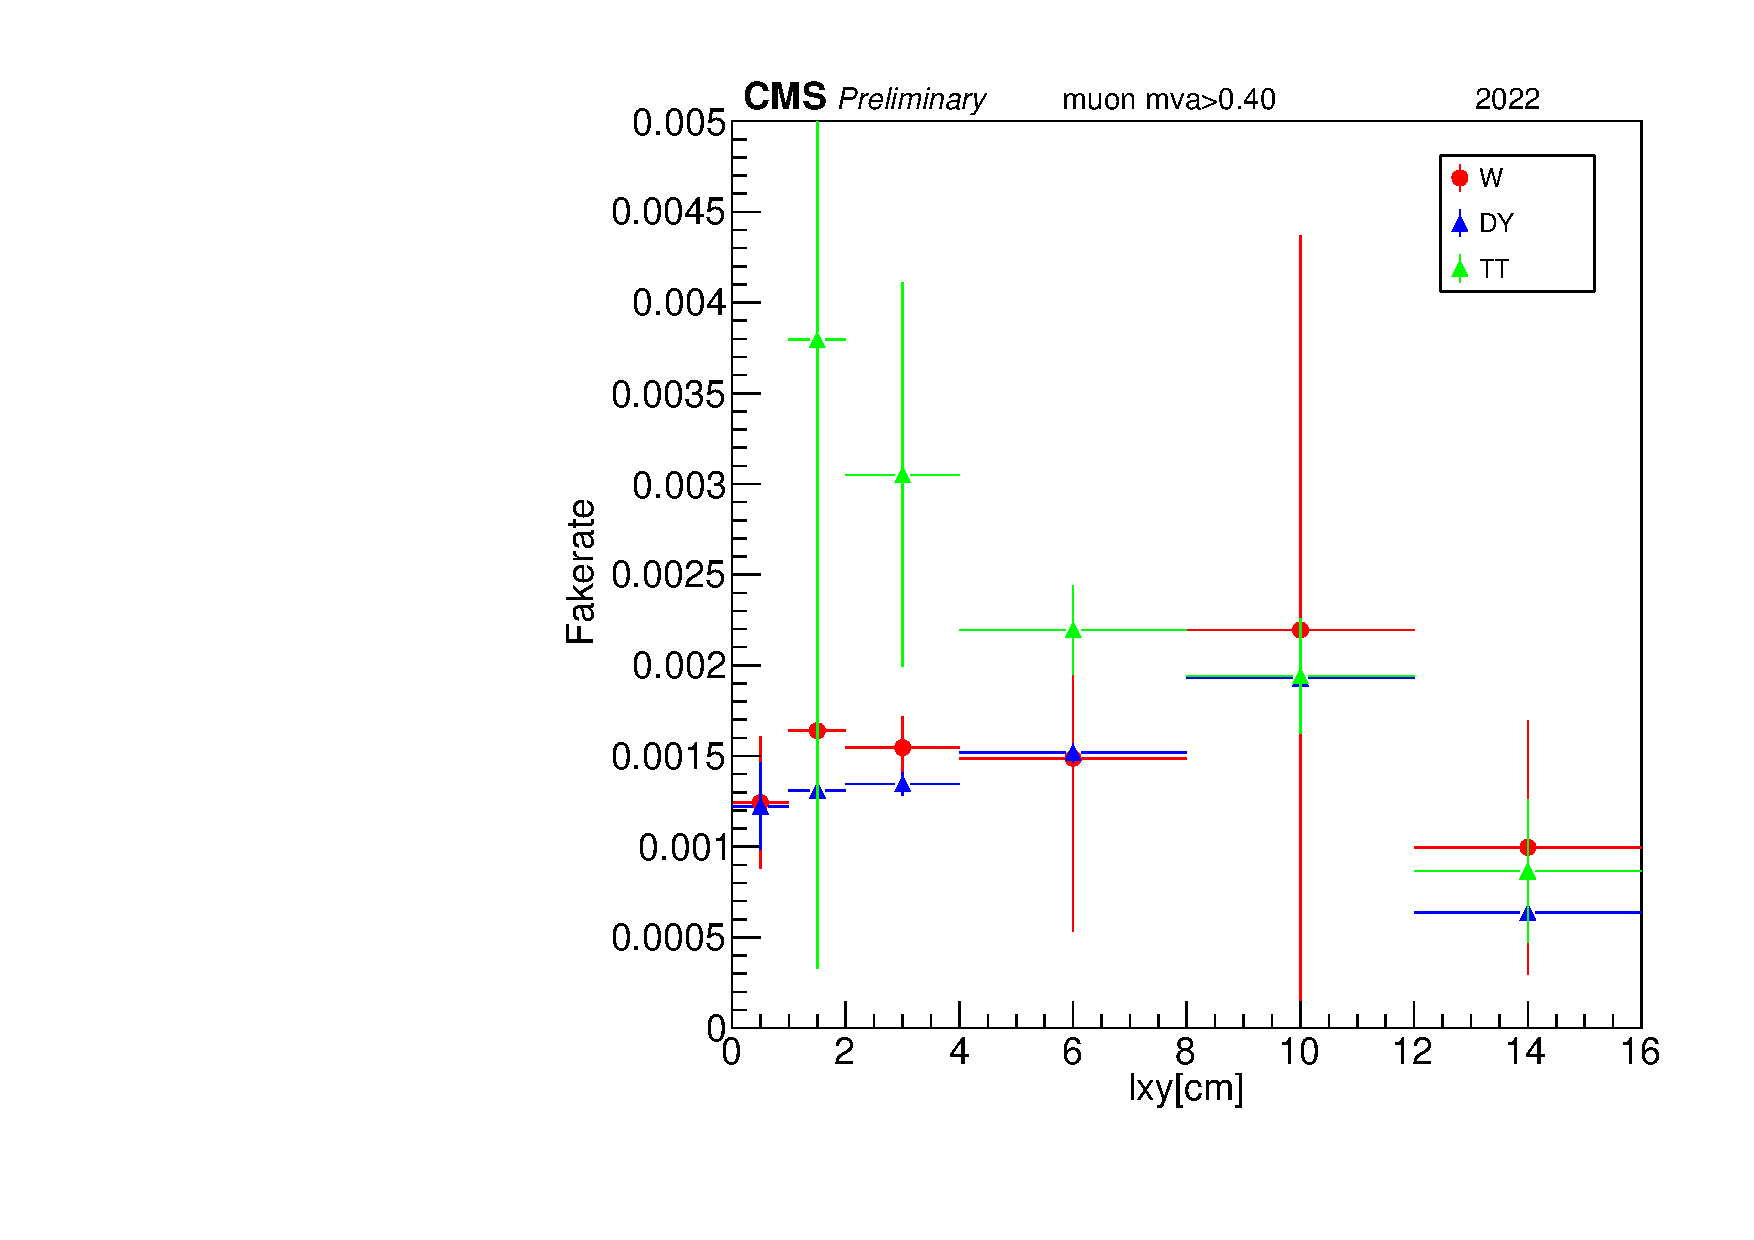
\includegraphics[width=0.45\textwidth]{figures/chapter4/fakerate/playV0-ks_kin_lxy_muidbdt40_W_v_DY_v_TT_overlay.pdf}
    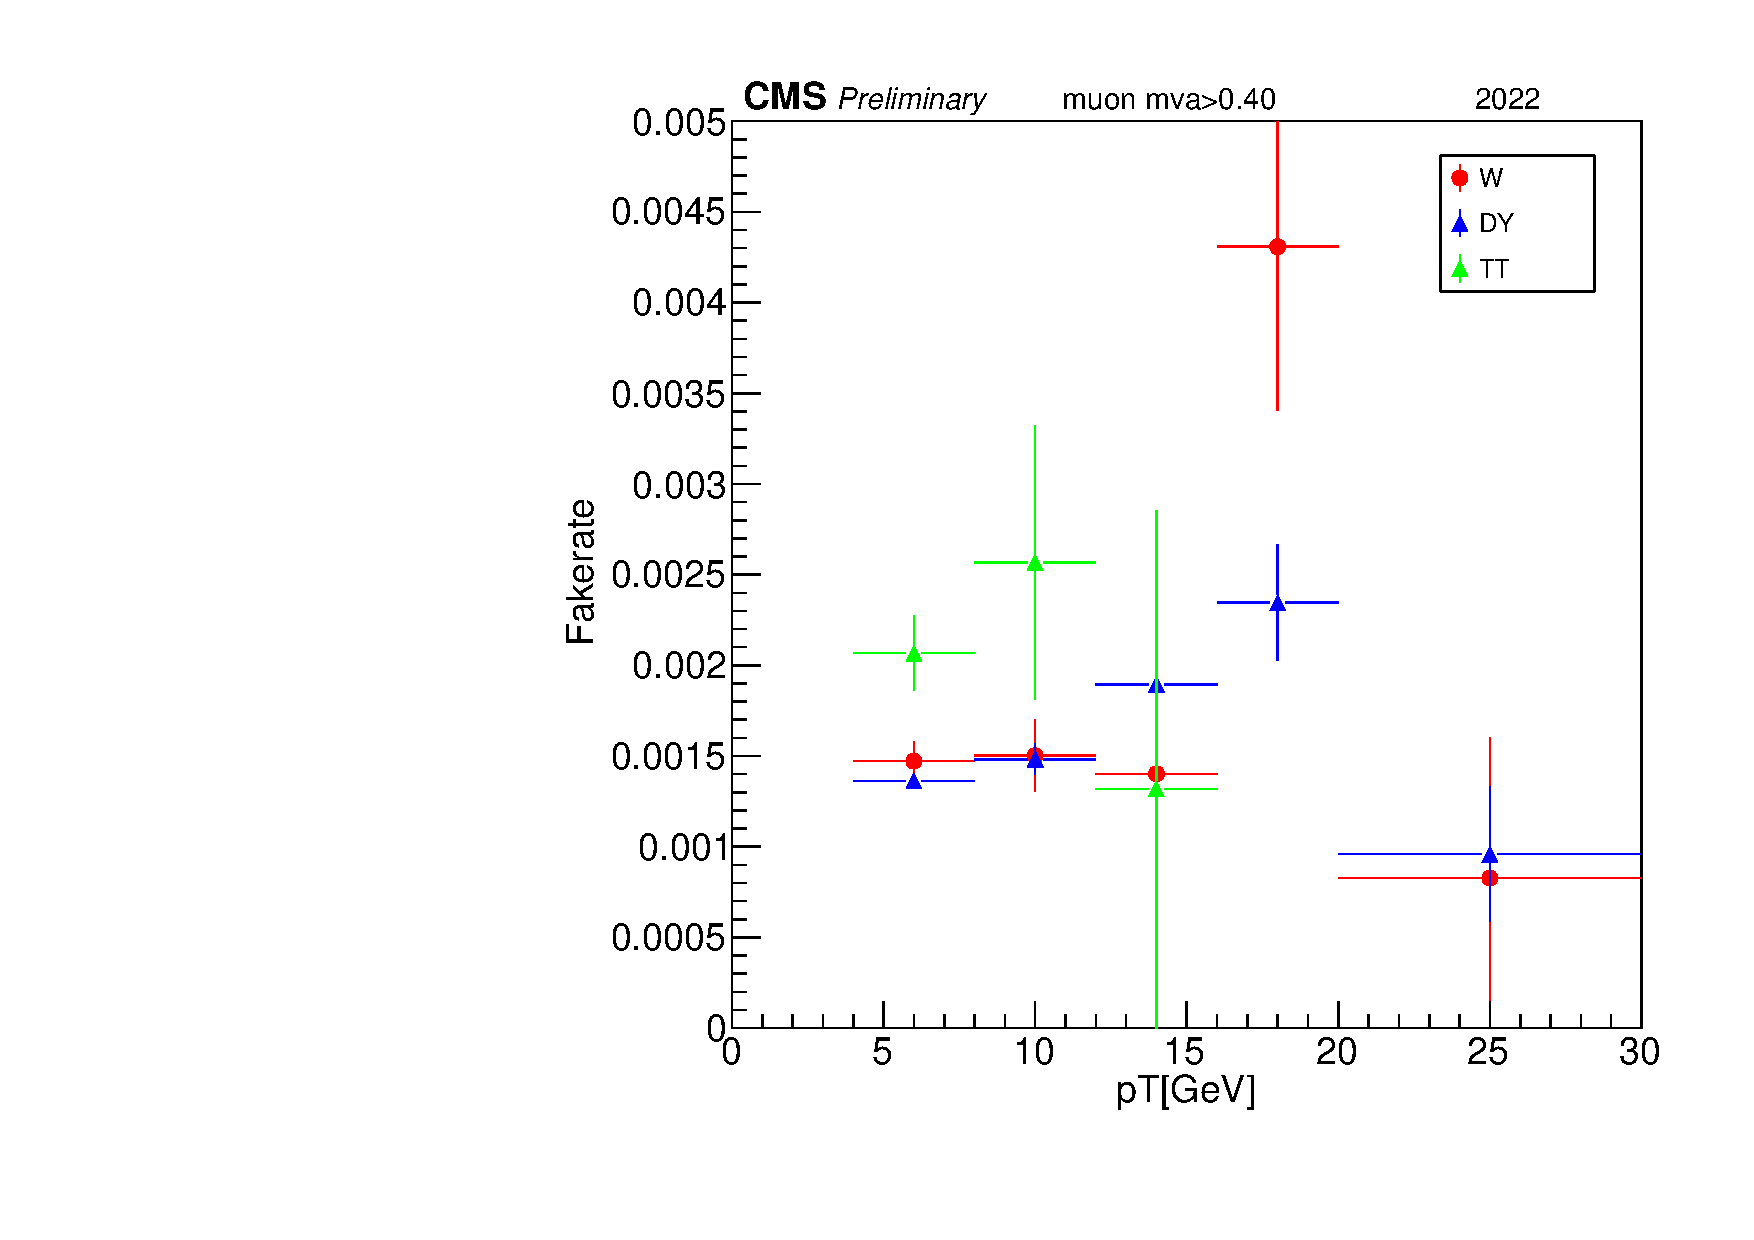
\includegraphics[width=0.45\textwidth]{figures/chapter4/fakerate/playV0-ks_kin_pT_muidbdt40_W_v_DY_v_TT_overlay.pdf}
  \end{center}
  \caption{Difference in fakerate between Egamma and Parking Electron data (top) and W plus jets, Drell-Yan, and TT bar MC samples (bottom) binned by flight length in cm (left) and pT in Gev (right)}
  \label{fig:pion_fake_rate_systematics}
\end{figure}

\begin{table}[htbp]
    \centering
    \begin{tabular}{|c|c|c|c|c|c|c|}
    \hline
     & \textbf{4--8 GeV} & \textbf{8--12 GeV} & \textbf{12--16 GeV} & \textbf{16--20 GeV} & \textbf{20--30 GeV} & \textbf{Total} \\
    \hline
    Run2022 & $1.05 \pm 0.03$ & $0.98 \pm 0.04$ & $1.11 \pm 0.09$ & $1.00 \pm 0.15$ & $1.38 \pm 0.46$ & $1.06 \pm 0.07$ \\
    Run2023 & $1.09 \pm 0.04$ & $0.95 \pm 0.04$ & $1.04 \pm 0.13$ & $1.08 \pm 0.17$ & $1.27 \pm 0.34$ & $1.03 \pm 0.07$ \\
    \hline
    \end{tabular}
    \caption{Muon fake rate ratios for Data over MC simulation for 2022 and 2023 in the bins of meson $p_\mathrm{T}$.}
    \label{tab:muon_fake_rate}
\end{table}


\section{Efficiency Corrections}
\label{sec:efficiency_corrections}

%TODO probably need to rewrite efficiency section in light of this section...

Virtually all selection efficiencies used for this analysis are measured in MC. Normally, this would be troublesome for the results of the analysis due to MC mismodeling effects that cause the efficiency of MC to be different from the efficiency of the data. In terms of a formula, we get that 
\begin{equation}
    \epsilon_{\text{data}} = \epsilon_{\text{MC}} \times \epsilon_{\text{corr}}
\end{equation}
with mismodeling occurring when $\epsilon_{corr} \neq 1$. 

However, the normalization channel approach used in this analysis means that in all calculations needed for the final result, we only care about a \textit{ratio} of efficiencies. One notices that if the $\epsilon_{\text{corr}}$ is the same for both the normalization and signal channels, it cancels when considering a ratio between normalization and signal channel efficiencies. In fact, we notice that except for trigger selection and $\text{MVA}_D$ selection, the selections are kept exactly the same between signal and normalization channels. Since the $\text{MVA}_D$ and trigger selections are independent of the other selections and independent of each other, we can let the other selection efficiency corrections cancel and only consider corrections to $\text{MVA}_D$ selection and trigger selection independently. The calculation of the $\text{MVA}_D$ correction, denoted $\text{MVA}_{D,corr}$ has already been discussed extensively in section \ref{subsec:mva}. Therefore, all that is left to consider is the trigger efficiency correction for both the $\texttt{HLT\_ZeroBias}$ trigger and the $\texttt{HLT\_DoubleMu4\_3\_LowMass}$ trigger. 

\subsection{Trigger Efficiency Correction}
\label{subsec:trigger_efficency_correction}

Trigger efficiency quantifies how often the trigger fires on events that the trigger is built to capture. For example, the efficiency of the $\texttt{HLT\_DoubleMu4\_3\_LowMass}$ trigger can be calculated as the percentage of low-mass dimuon events that are successfully captured by the trigger. As discussed in section \ref{sec:efficiency_corrections}, the trigger efficiency correction is the ratio of the trigger efficiency in data over the trigger efficiency in MC, used to account for MC mismodeling effects. For our analysis, the trigger efficiency correction of both the $\texttt{HLT\_ZeroBias}$ trigger and the $\texttt{HLT\_DoubleMu4\_3\_LowMass}$ trigger must be found. However, by definition, the $\texttt{HLT\_ZeroBias}$ trigger selects events with no bias, therefore it has $100\%$ efficiency in both data and MC, causing its trigger efficiency correction to be 1. Therefore, in this analysis we only calculate the trigger efficiency correction of the $\texttt{HLT\_DoubleMu4\_3\_LowMass}$ trigger and label it $T_{\text{cor}}$. As is covered in section \ref{sec:triggers}, the triggers are split up into HLT and L1 triggering systems. Therefore, it is convenient for us to calculate their efficiency corrections separately and then combine them to get $T_{\text{cor}} = T_{\text{cor, L1}} \times T_{\text{cor, HLT}}$.

Calculating trigger efficiency in MC samples is done by simply calculating how many of the generated events that fit the trigger criterion actually fired the trigger. In data, we don't know how many events there actually were that fit a certain criterion, making this straight-forward calculation impossible. Instead, in data we calculate the trigger efficiency of one trigger with respect to another which we know has virtually $100\%$ efficiency. Specifically, we calculate what percentage of the time the trigger of interest fired for all events where the reference trigger has also fired. For consistency, then, the MC trigger efficiency is calculated using this same method, instead of the straight forward method initially described. Note that when calculating trigger efficiencies, one must carefully take into account trigger prescales, making sure to equate the scaling of both the trigger of interest and reference trigger. Additionally, since the triggers were changed slightly between 2022 and 2023, we calculate the trigger efficiency corrections in each year separately and then combine to get a total efficiency correction.

We begin with calculating the L1 trigger efficiency correction. The $\texttt{HLT\_DoubleMu4\_3\_LowMass}$ trigger has two L1 triggers it uses for selecting muons, named $\texttt{HLT\_Mu4\_L1DoubleMu}$ and $\texttt{HLT\_Mu0\_L1DoubleMu}$. For the L1 trigger efficiency correction calculation, we pick using $\texttt{HLT\_Mu0\_L1DoubleMu}$ and use the other trigger to find the HLT trigger efficiency correction. For the reference trigger, we use $\texttt{HLT\_Mu3\_PFJet40}$ and $\texttt{HLT\_Mu8}$, both intended for L1 trigger efficiency studies. These triggers both have a single muon efficiency of $0.8714$, meaning that the dimuon efficiency can be calculated to be $1- (1-\sqrt{0.8714})^2 = 0.996 \approx 1$. 

Next, we calculate the HLT trigger efficiency correction, or the fraction of events that pass $\texttt{HLT\_DoubleMu4\_3\_LowMass}$ given that they've passed one of the L1 triggers, $\texttt{HLT\_Mu4\_L1DoubleMu}$. By definition, this means that we can use the $\texttt{HLT\_DoubleMu4\_3\_LowMass}$ trigger with respect to the  $\texttt{HLT\_Mu4\_L1DoubleMu}$ trigger to calculate the HLT trigger efficiency. 

The results of these calculations are summarized in table \ref{tab:trigger_efficiency}. Putting these results together, the correction derived for the L1 trigger is $0.990 \pm 0.005$ and the correction derived for the HLT trigger is $0.953 \pm 0.005$. Put together, this results in a total corrective factor of $T_{\text{cor}} = 0.943 \pm 0.007$. 

\begin{table}[ht]
    \centering
    \begin{tabular}{|>{\footnotesize\raggedright\arraybackslash}p{10cm}|c|c|c|}
    \hline
    \textbf{Measurement} & \multicolumn{2}{c|}{\textbf{Efficiency (\%)}} & \textbf{Ratio} \\
    \cline{2-3}
    & \textbf{Data} & \textbf{MC} & \\
    \hline
    \multicolumn{4}{|c|}{\textbf{2022}} \\
    \hline
    HLT\_DoubleMu4\_3\_LowMass \textbf{wrt} HLT\_Mu4\_L1DoubleMu & $90.08 \pm 0.15$ & $94.91 \pm 0.09$ & $0.949 \pm 0.002$ \\
    HLT\_Mu0\_L1DoubleMu \textbf{wrt} HLT\_Mu3\_PFJet40 & $88.61 \pm 0.60$ & $88.72 \pm 0.43$ & $0.999 \pm 0.008$ \\
    HLT\_Mu0\_L1DoubleMu \textbf{wrt} HLT\_Mu8 & $90.51 \pm 0.25$ & $91.39 \pm 0.18$ & $0.990 \pm 0.003$ \\
    \hline
    \multicolumn{4}{|c|}{\textbf{2023}} \\
    \hline
    HLT\_DoubleMu4\_3\_LowMass \textbf{wrt} HLT\_Mu4\_L1DoubleMu & $90.76 \pm 0.15$ & $94.91 \pm 0.09$ & $0.956 \pm 0.002$ \\
    HLT\_Mu0\_L1DoubleMu \textbf{wrt} HLT\_Mu3\_PFJet40 & $87.88 \pm 0.67$ & $88.72 \pm 0.43$ & $0.990 \pm 0.009$ \\
    HLT\_Mu0\_L1DoubleMu \textbf{wrt} HLT\_Mu8 & $90.10 \pm 0.20$ & $91.39 \pm 0.18$ & $0.986 \pm 0.003$ \\
    \hline
    \end{tabular}
    \caption{Trigger efficiency measurements in Data and MC for 2022 and 2023.}
    \label{tab:trigger_efficiency}
\end{table}

\section{Results}

\subsection{The $CL_s$ Method}

The final result of this thesis is presented as a $CL_s$ limit. Therefore, before discussing the results of the thesis I will describe briefly what the $CL_s$ limit is, why it is used, and how to calculate it. 

Modern statistics utilizes two main frameworks for interpreting search results. The first of these frameworks is a Bayesian framework, developed by calculating posteriors using likelihoods generated from data and inferred priors. However, defining priors over complex or untested hypothesis proves difficult and becomes very subjective to the method in which researchers assign priors. Therefore, for many applications, such as this one, the Bayesian approach is incomplete. The second of these frameworks is the frequentist approach, which draws conclusions on the compatibility of data with a given theory. However, in nearly all physical applications, researchers aim to generate conclusions on theory given data. Due to the convergence of Bayesian and frequentist conclusions in experiments with large signals and high backgrounds, researchers often allow themselves to draw conclusions on theory with a frequentist approach. However, this method will not hold here due to the incredibly small signal we are searching for.

To figure out what technology to use instead of these methods, we analyze carefully what goes wrong with a standard confidence interval test. The fundamental problem of these tests is that without proper prior weighting of hypothesis, one rejects hypothesis which the experiment had no sensitivity to. More specifically, confidence intervals can tell you about the validity of a hypothesis without considering how likely it is that the hypothesis can be proven wrong. This is what the $CL_s$ method fixes; it takes the p-value of the signal+background model used in confidence intervals and divides it by the one minus p-value of the background. Therefore, if the model for the signal+background hypothesis is close to the model for the background-only hypothesis, the $CL_s$ method imposes a penalty due to the lack of sensitivity in the experiment. 

The fundamental building block for the $CL_s$ method is the likelihood ratio test statistic, 
\begin{equation}
    Q = -2 \ln \left(\frac{\mathcal{L}(s+b)}{\mathcal{L}(b)}\right)
\end{equation}
where $\mathcal{L}(s+b)$ is the likelihood calculated by the UML fit described in section \ref{sec:UML} and $\mathcal{L}(b)$ is the likelihood calculated using the same fit but excluding the signal model. This means that small $Q$ values correspond to fits that indicate a stronger signal+background fit than background-only fit. 

Now, recall from section \ref{sec:UML} that the likelihood is dependent on the nuisance parameters as well as the parameter of interest. Therefore, we adjust our notation briefly to reflect this, writing $\mathcal{L}_{(b)}(\theta, \vec{\theta}_N)$ and $\mathcal{L}_{(s+b)}(\theta, \vec{\theta}_N)$ to represent the likelihoods. In this experiment, like many others, there are many nuisance parameters that complicate the shape of the likelihood, increase computational complexity, and cause us to track an unmanageable amount of uncertainties. To avoid these issues, we introduce the profile likelihood, $\mathcal{L}_p(\theta) = \max_{\vec{\theta}_N} \mathcal{L}(\theta, \vec{\theta}_N)$. Note that this is not a real likelihood due to the fact that it does not reflect uncertainties in nuisance parameters. However, the test statistic $Q_p$ obtained from the profile likelihood ratio is equivalent to the full likelihood ratio test statistic. For this reason, in virtually every analysis (including this one) the profile likelihood is used. Additionally, due to the lack of impact on the validity of the test statistic, we drop that $\mathcal{L}_p$ and $Q_p$ notation for the remainder of the discussions in this thesis. However, it is important to remember that we are always using profile likelihoods instead of true likelihoods in this analysis. 

Now that we have generated the basic formalism needed to discuss $CL_s$ methods, there are two main applications of $CL_s$ that are used in every experiment. These applications are (i) scanning analysis variables for the best expected limit and (ii) finding the bound of the parameter of interest based on unblinded data. Both these applications are discussed below and later applied to the analysis in section \ref{subsec:sensitivity_scan} and section \ref{subsec:final_result}.

\subsubsection{Limit Calculation Using Real Data}
\label{subsubsec:limit_calculation_theory}

In many $CL_s$ experiments, the goal is to put a limit on a parameter of a physical theory using observed data. This is typically done once the entire analysis has been frozen and only the unblinding is left. Before starting the $CL_s$ method, one picks the confidence level that you would like to have, denoted $CL$. Common $CL$ values are $90\%$ and $95\%$. 

To begin, $n$ toy experiments are generated under a background-only hypothesis and for each of these toys, a $Q$ value is generated, giving a distribution of $n$, $Q_b$ values. In the case of this analysis, this is straight forward since our background model is in the form of a PDF as described in section \ref{sec:UML}. Therefore, one simply samples from the background PDF to generate background-only toy data. 

Once the background-only test statistic distribution is complete, one generates a singular $Q_{\text{obs}}$ value based on the actual, observed data. The area under the curve of the $b$ distribution to the left of $Q_{\text{obs}}$ is then calculated and is the $p_b$ value.

Next, $n$ more toy experiments are generated under a signal+background hypothesis, where the signal strength, $s$, is left floating. These toy experiments are constructed using a similar method to the backgrounds, just with the signal+background model for some signal strength, $s$. We denote this distribution of $n$ points $Q_{s+b}(s)$, highlighting its dependence on $s$, the signal strength. From this, the area under the curve of $s+b$ distribution to the right of $Q_{\text{obs}}$ is the p-value (or $p_{s+b}(s)$ value, again denoting the dependence on $s$). 

Then, the $CL_s(s)$ value is determined by calculating
\begin{equation}
    CL_s(s) = \frac{p_{s+b}(s)}{1-p_b}
\label{eq:cls}
\end{equation}
Lastly, the value of $s$ is found such that $CL_s(s) = 1-CL$\footnote{It may seem computationally difficult to do this naively by scanning over $s$ values and generating $n$ toys for each value of $s$. While optimizations exists in certain cases, employing $CL_s$ methods is in practice computationally challenging}. This value of $s$ is then reported as the upper limit. An example of this can be seen in figure \ref{fig:cls_visualization}.

\begin{figure}[h!]
    \begin{center}
      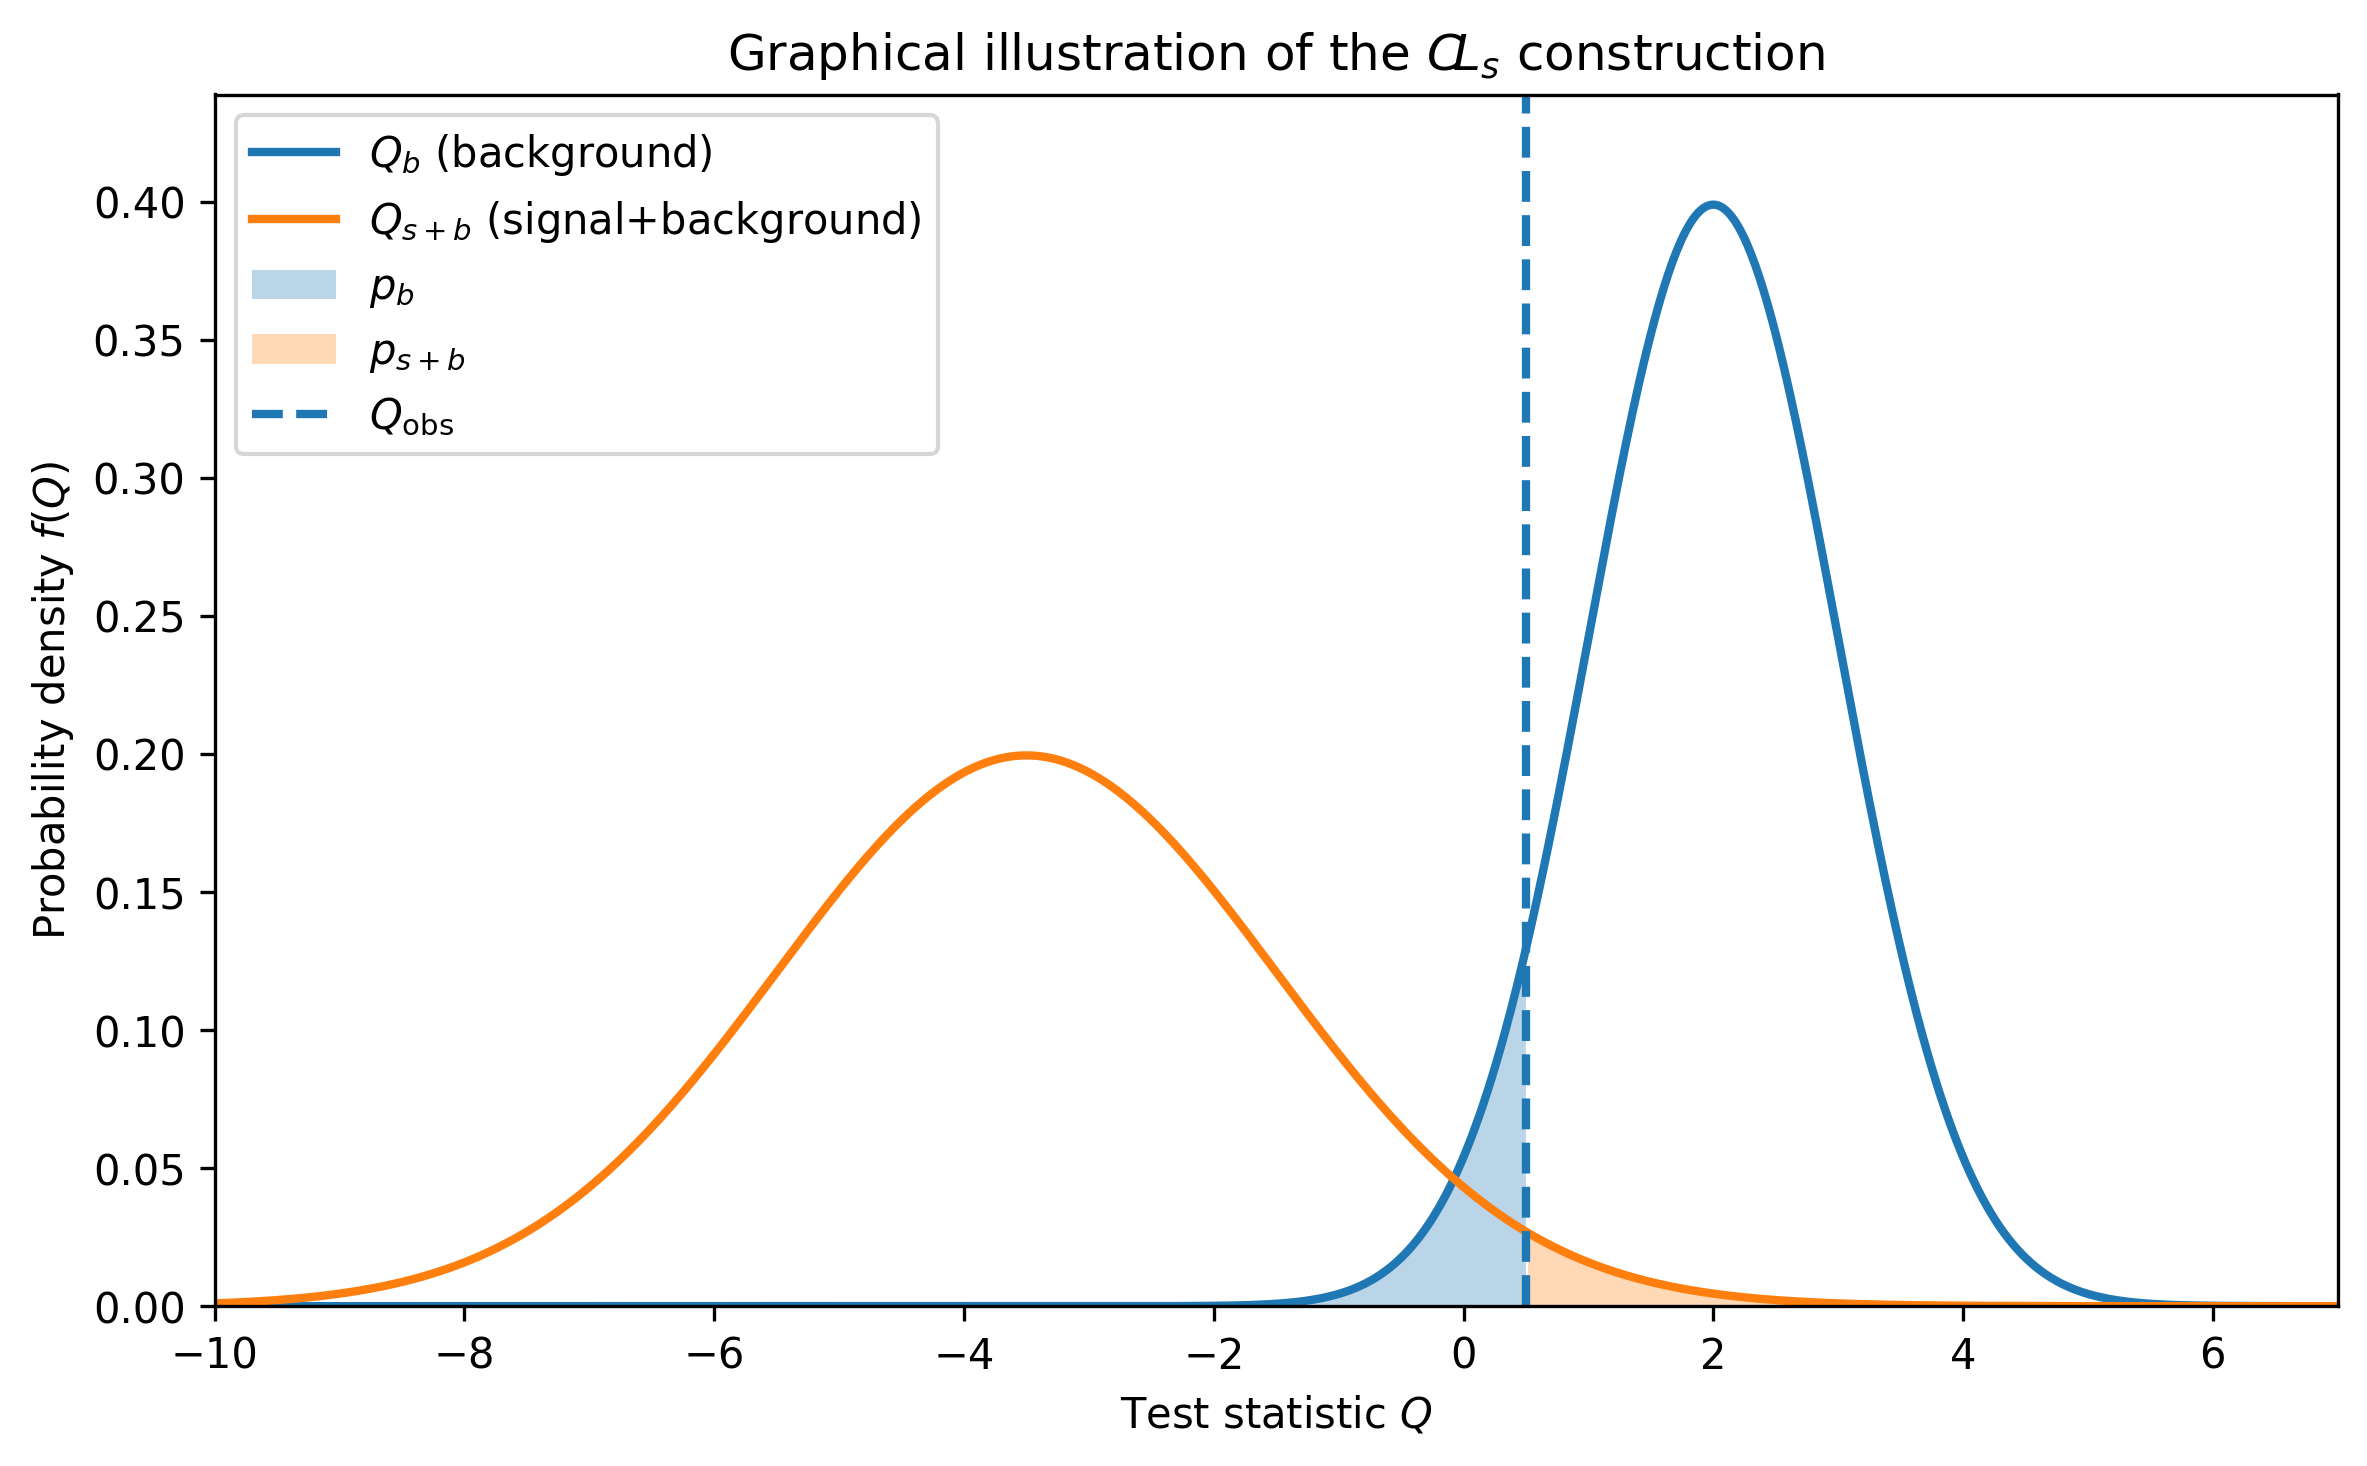
\includegraphics[width=0.8\textwidth]{figures/chapter4/cls_visualization.png}
    \end{center}
    \caption{
      A visualization of the $CL_s$ method, using idealized data and a given signal strength, $s$. 
    }
    \label{fig:cls_visualization}
\end{figure}

\subsubsection{Sensitivity Scanning Using Expected Limits}
\label{subsubsec:sensitivity_scanning_limits}

In many $CL_s$ experiments (including this one), one is interested in tuning a parameter, $\alpha$, in the analysis to get the best experimental outcome. However, this cannot be done directly once the data is unblinded, since this would introduce bias by allowing the observed data to influence the optimization, leading to overfitting. Instead, sensitivity scans are performed using expected limits. To begin, one picks several discrete values of parameter $\alpha$ to test, labeled $\alpha_i$. As before, one additionally picks desired confidence level.

For simplicity, let's assume, for now, that we are not interested in keeping our data blinded during the sensitivity scan and directly have access to the data and therefore $Q_{\text{obs}}$. In this case, the sensitivity scan becomes a straight forward extension of the previous section. Namely, for each $\alpha_i$, distributions of $Q_b$ and $Q_{s+b}(s)$ are generated, the value of $Q_{\text{obs}}$ is obtained given $\alpha_i$, the $CL_s(s)$ value is calculated, and the value of $s$ is found such that $CL_s(s) = 1-CL$. Then, the specific $\alpha_i$ is picked that generates the most sensitive $s$. 

In the case where we don't have access to the real data, we must compute an expected result given simulated data under a given hypothesis. It is common for searches to use background-only hypothesis for this, given that there is typically much evidence for the background-only hypothesis, though more complex choices are possible\footnote{One may be concerned about the freedom of choice for a reference hypothesis. However, recall that this doesn't affect the final limit calculation, just the choice of $\alpha$ that generates the best model sensitivity. If one picks the "wrong" reference hypothesis, one simply finds a worse choice of $\alpha$. In practice, however, most reasonable choices work here to find a good value of $\alpha$.}. There are then two options for computing $Q_{\text{pseudo-observed}}$ to be used instead of $Q_{\text{obs}}$. The first is to again generate toys under the hypothesis of choice to get a distribution of $Q$ values, then take the median of that distribution to get $Q_{\text{pseudo-observed}}$. The second is to generate an Asimov dataset, by simply generating a "perfect" dataset with no statistical fluctuations on the background only model and computing the $Q$ value of this "perfect" dataset. Importantly, this is much cheaper computationally, but requires the conclusion that the median of the toy results is equivalent to the toy result of the median, which requires a Gaussian approximation. In practice, this approximation is typically valid (as is the case in this analysis), so the Asimov dataset approach is used.

There is one more subtlety that is worth addressing to complete the $CL_s$ picture. Wilks' theorem states that the profile likelihood ratio, $Q$, distributes asymptotically as a $\chi^2$ distribution with degrees of freedom equal to the difference in the number of floating variables in the signal+background model compared to the background-only model. This implies that, under the asymptotic and null assumption, one doesn't need to generate distributions of $Q_b$ using toys. Instead, one can always use Wilks' theorem to derive the shape of the $Q_b$ distribution from a $\chi^2$ distribution. In practice, this approximation is also well-founded and used in most sensitivity scans, dramatically reducing the number of toys needed. 

\subsection{Sensitivity Scan}
\label{subsec:sensitivity_scan}

Now that the statistical formulation for the final result is complete, we turn back to the calculation of the final result. 

As mentioned in section \ref{subsec:mva}, one of the major benefits of using an $\text{MVA}_D$ cut parameter is that we can tune it to best improve analysis sensitivity. This is done using the technology developed in section \ref{subsubsec:sensitivity_scanning_limits} with two important distinctions to highlight.

Firstly, one might assume that the parameter of interest is the output of the signal channel UML fit, $N_{D^0 \to \mu^+ \mu^-}$. However, this is not quite true as the parameter that we wish to put a limit on is the actual branching fraction $\mathcal{B}(D^0 \to \mu^+ \mu^-)$. The discussion in section \ref{subsec:signal_channel_uml} can be extended to the calculation of $\mathcal{B}(D^0 \to \mu^+ \mu^-)$, resulting in 
\begin{equation}
    \frac{N_{D^0 \to \mu^+  \mu^-}}{N_{D^0 \to \pi^+ \pi^-}} = \frac{\mathcal{B}(D^0 \to \mu^+ \mu^-)}{\mathcal{B}(D^0 \to \pi^+ \pi^-)}\times \frac{\epsilon_{D^*, D^0\to\mu\mu}}{\epsilon_{D^*, D^0\to\pi\pi}} \times S_{ZB} \times \text{MVA}_D \times T_{\text{corr}} 
\end{equation}
where the variables are the same as defined in equation \ref{eq:peaking_background_yield_calculation}. Therefore, to perform the sensitivity scan we don't just calculate $N_{D^0 \to \mu^+ \mu^-}$ under different toy experiments, but rather perform the entire calculation required to derive $\mathcal{B}(D^0 \to \mu^+ \mu^-)$, including the calculation of $\epsilon_X$ and $N_{D^0 \to \pi^+ \pi^-}$ at various $\text{MVA}_D$ working points. Luckily, there are some parameters that don't change, such as $T_{\text{corr}}$ or $S_{ZB}$, so some computation can be saved.

The other important distinction is that under the $\texttt{HLT\_ZeroBias}$ trigger, there are simply too few data points to produce an effective sensitivity scan result. Therefore, to avoid being biased by data fluctuations that prevail when signal events are rare, we include five additional zero bias data. The five triggers of corresponding to the datasets is listed below
\begin{enumerate}
    \item \texttt{HLT\_ZeroBias\_FirstBXAfterTrain}
    \item \texttt{HLT\_ZeroBias\_FirstCollisionAfterAbortGap}
    \item \texttt{HLT\_ZeroBias\_FirstCollisionInTrain}
    \item \texttt{HLT\_ZeroBias\_IsolatedBunches}
    \item \texttt{HLT\_ZeroBias\_LastCollisionInTrain}
\end{enumerate}
An important note is that these additional datasets are not used in the calculation of the final limit, due to an incomplete understanding of how their additional requirements could affect the analysis. However, the effects are assumed to be small enough that they still provide valuable insight to determine what $\text{MVA}_D$ working point to use. 

The results of this scan are shown in figure \ref{fig:sensitivity_scan}. The best $\text{MVA}_D$ cut values can be seen to be in the range 0.74 to 0.84. In order to include as many signal events as possible, we choose the loosest $\text{MVA}_D$ cut in this range at $0.74$ for the final value to be used to maximize analysis sensitivity. 

\begin{figure}[h!]
    \begin{center}
      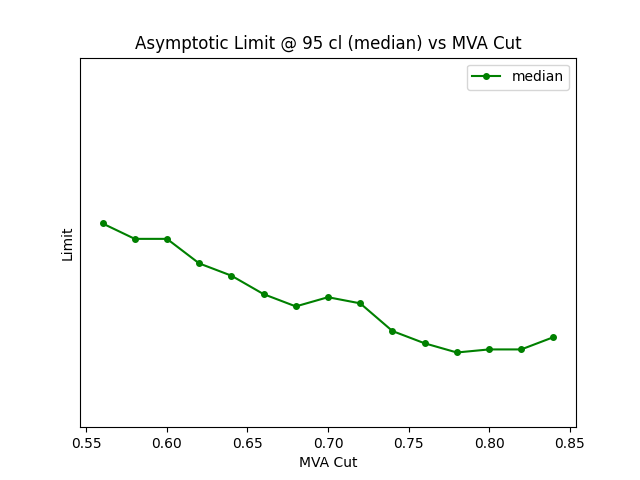
\includegraphics[width=0.45\textwidth]{figures/chapter4/results/limit_bdt_median.png}
      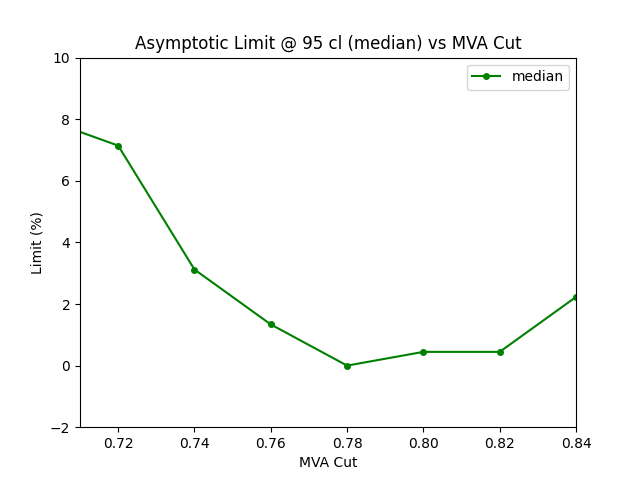
\includegraphics[width=0.45\textwidth]{figures/chapter4/results/limit_bdt_median_v2.png}\\
    \end{center}
    \caption{
      The sensitivity scan against various MVA cuts first within a broad range of MVA cut values (left) and then with a more concentrated range of MVA cut values (right).
    }
    \label{fig:sensitivity_scan}
\end{figure}

\subsection{Branching Fraction Limit}
\label{subsec:final_result}

Finally, we present the final result. After applying the formalism developed in section \ref{subsubsec:limit_calculation_theory} and unblinding the data, we find that the upper limit on the branching fraction at a $90(95)\%$ confidence level is
\begin{equation}
    \mathcal{B}(D^0 \to \mu^+ \mu^-) < 2.1(2.4) \times 10^{-9} 
\end{equation}
Table \ref{tab:final_observed_yeild} shows the central values of the observed yields for each decay channel studied in this analysis and figure \ref{fig:final_observed_fit} displays the final fit on the observed data.

\begin{table}[h!]
    \centering
    \begin{tabular}{|l|c|}
    \hline
    \textbf{Observed Yields} & \textbf{Values} \\
    \hline
    $N_{D^0 \rightarrow \mu^+\mu^-}$ & $139 \pm 123$ \\
    $N_{D^0 \rightarrow \pi^+\pi^-}$ & $220 \pm 58$ \\
    $N_{D^0 \rightarrow \pi^-\mu+\nu_\mu}$ & $207 \pm 40$ \\
    $N_{\text{comb}}$ & $126185 \pm 366$ \\
    $N_{\text{total}}$ & 126752 \\
    \hline
\end{tabular}
\caption{The final observed yield, based on data.}
\label{tab:final_observed_yeild}
\end{table}

\begin{figure}[h!]
    \begin{center}
      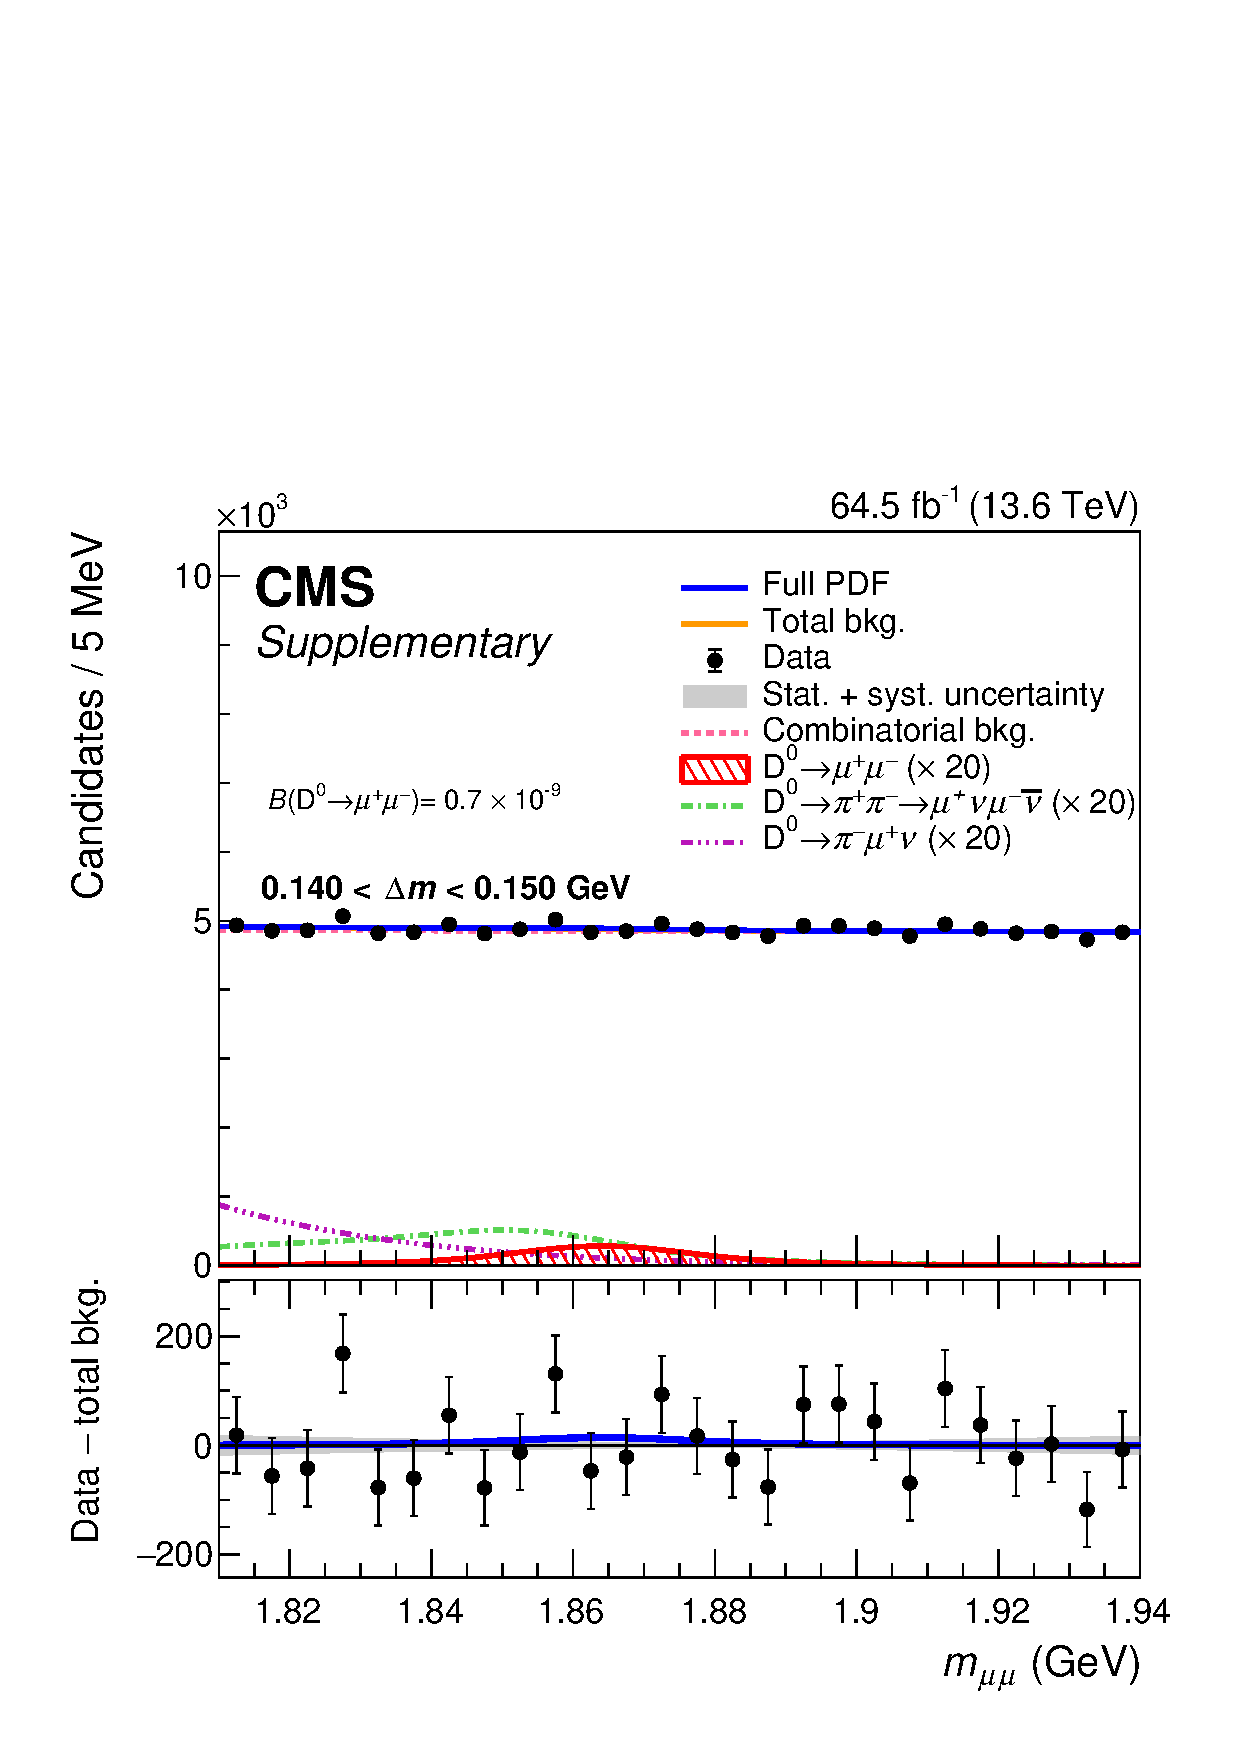
\includegraphics[width=0.45\textwidth]{figures/chapter4/results/SB_plot_m_full_test.pdf}
      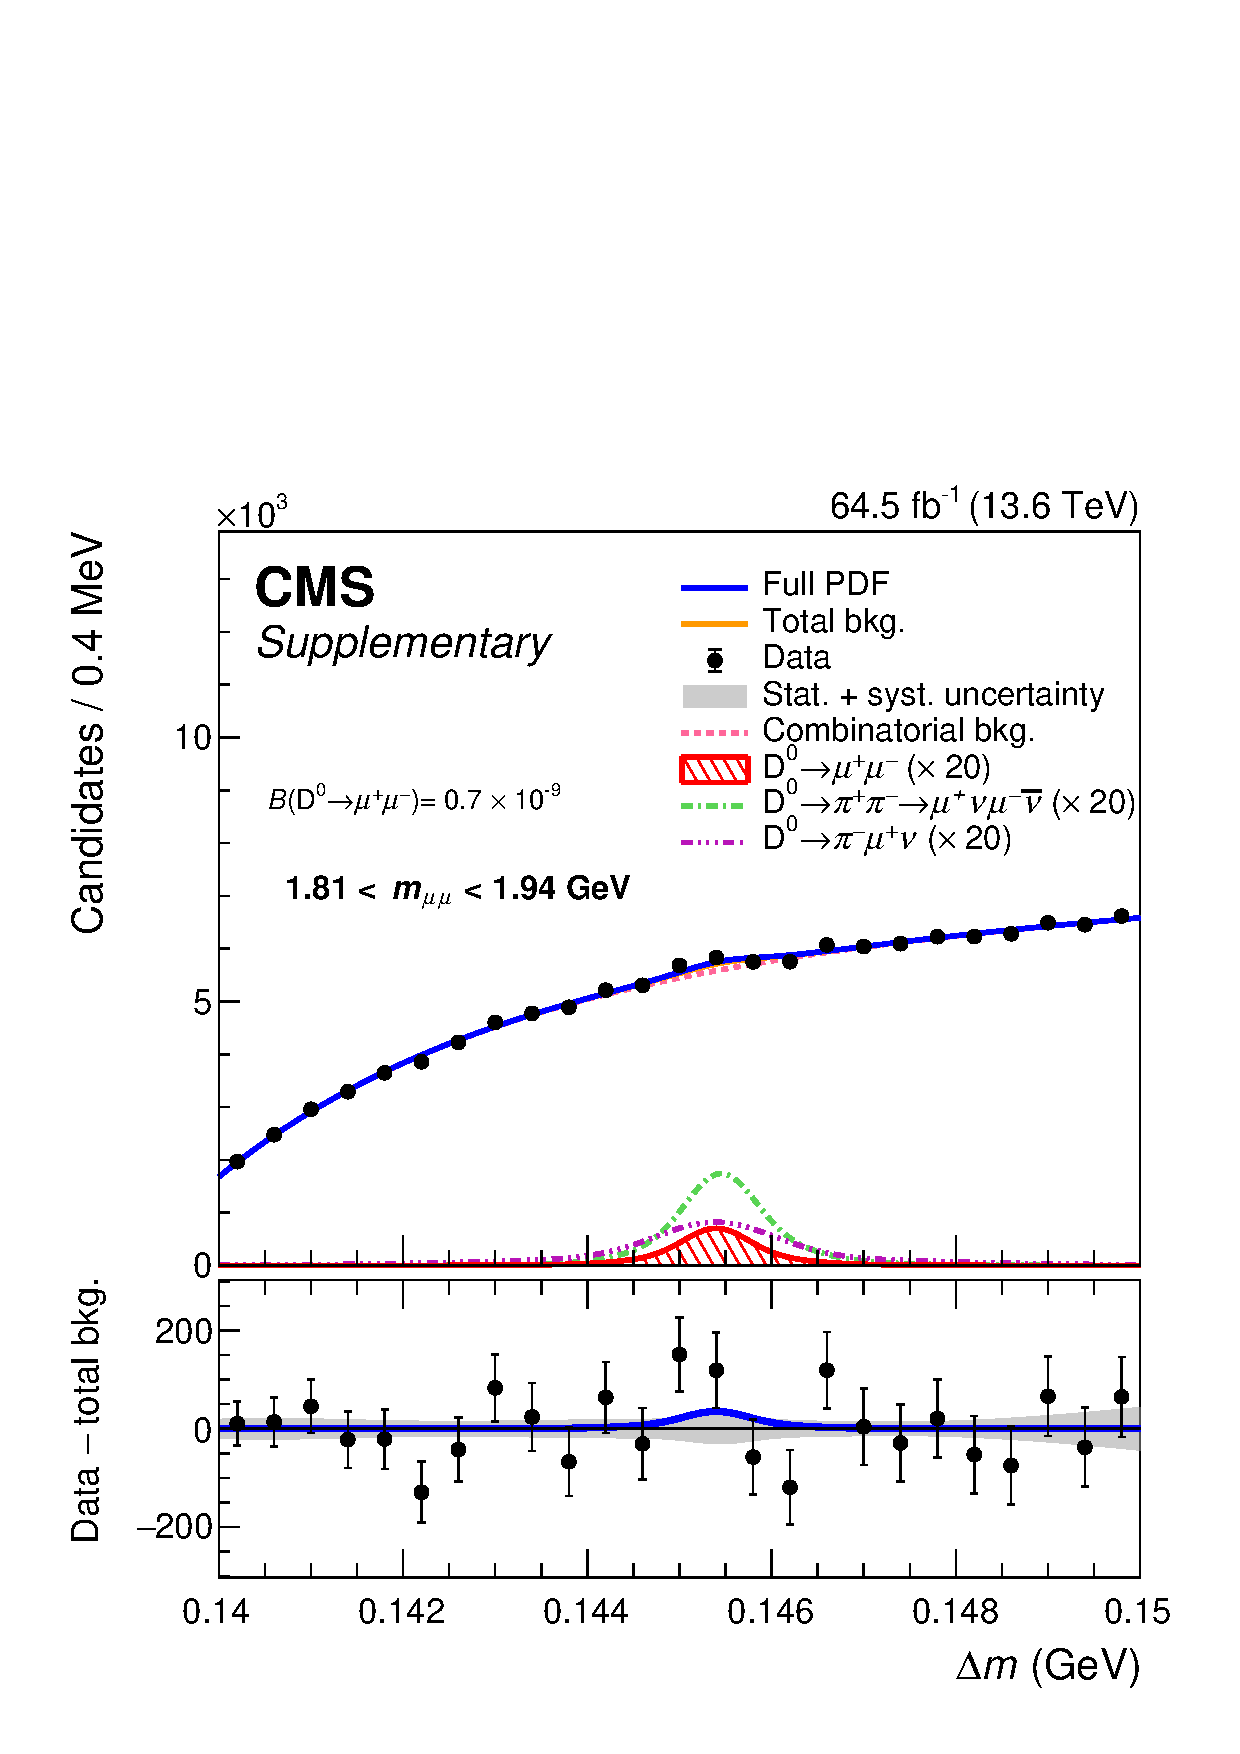
\includegraphics[width=0.45\textwidth]{figures/chapter4/results/SB_plot_dm_full_test.pdf}\\
    \end{center}
    \caption{
      The unblind fit on observed data shown in $m(D^0)$ (left) and $\Delta m$ (right). Note that the peaking decays are visually scaled by a factor of 20.
    }
    \label{fig:final_observed_fit}
  \end{figure}